%DIF 1-2c1-23
%DIF LATEXDIFF DIFFERENCE FILE
%DIF DEL ../g3_v1/g3_v1.tex         Tue Feb 16 19:01:39 2021
%DIF ADD ../g3_v2/coupling_v2.tex   Wed Feb 17 02:29:02 2021
%DIF < % Kerswell et al. Coupling G3 submission June 2020
%DIF < \documentclass[draft]{assets/agujournal2019}
%DIF -------
%% March 2018 %DIF >
%%%%%%%%%%%%%%%%%%%%%%%%%%%%%%%%%%%%%%%%%%%%%%%%%%%%%%%%%%%%%%%%%%%%%%%%%%%% %DIF >
% AGUJournalTemplate.tex: this template file is for articles formatted with LaTeX %DIF >
% %DIF >
% This file includes commands and instructions %DIF >
% given in the order necessary to produce a final output that will %DIF >
% satisfy AGU requirements, including customized APA reference formatting. %DIF >
% %DIF >
% You may copy this file and give it your %DIF >
% article name, and enter your text. %DIF >
% %DIF >
% %DIF >
% Step 1: Set the \documentclass %DIF >
% %DIF >
% There are two options for article format: %DIF >
% %DIF >
% PLEASE USE THE DRAFT OPTION TO SUBMIT YOUR PAPERS. %DIF >
% The draft option produces double spaced output. %DIF >
% %DIF >
 %DIF >
%% To submit your paper: %DIF >
\documentclass[draft,linenumbers]{agujournal2018} %DIF >
\usepackage{apacite} %DIF >
%DIF -------
\usepackage{url} %this package should fix any errors with URLs in refs.
%DIF 4-5c25-102
%DIF < \usepackage{lineno}
%DIF < \usepackage{soul}
%DIF -------
%%%%%%% %DIF >
% As of 2018 we recommend use of the TrackChanges package to mark revisions. %DIF >
% The trackchanges package adds five new LaTeX commands: %DIF >
% %DIF >
%  \note[editor]{The note} %DIF >
%  \annote[editor]{Text to annotate}{The note} %DIF >
%  \add[editor]{Text to add} %DIF >
%  \remove[editor]{Text to remove} %DIF >
%  \change[editor]{Text to remove}{Text to add} %DIF >
% %DIF >
% complete documentation is here: http://trackchanges.sourceforge.net/ %DIF >
%%%%%%% %DIF >
 %DIF >
 %DIF >
%% Enter journal name below. %DIF >
%% Choose from this list of Journals: %DIF >
% %DIF >
% JGR: Atmospheres %DIF >
% JGR: Biogeosciences %DIF >
% JGR: Earth Surface %DIF >
% JGR: Oceans %DIF >
% JGR: Planets %DIF >
% JGR: Solid Earth %DIF >
% JGR: Space Physics %DIF >
% Global Biogeochemical Cycles %DIF >
% Geophysical Research Letters %DIF >
% Paleoceanography and Paleoclimatology %DIF >
% Radio Science %DIF >
% Reviews of Geophysics %DIF >
% Tectonics %DIF >
% Space Weather %DIF >
% Water Resources Research %DIF >
% Geochemistry, Geophysics, Geosystems %DIF >
% Journal of Advances in Modeling Earth Systems (JAMES) %DIF >
% Earth's Future %DIF >
% Earth and Space Science %DIF >
% Geohealth %DIF >
% %DIF >
% ie, \journalname{Water Resources Research} %DIF >
 %DIF >
\journalname{Geochemistry, Geophysics, Geosystems} %DIF >
 %DIF >
% Pandoc citation processing %DIF >
\newlength{\csllabelwidth} %DIF >
\setlength{\csllabelwidth}{3em} %DIF >
\newlength{\cslhangindent} %DIF >
\setlength{\cslhangindent}{1.5em} %DIF >
% for Pandoc 2.8 to 2.10.1 %DIF >
\newenvironment{cslreferences}% %DIF >
  {}% %DIF >
  {\par} %DIF >
% For Pandoc 2.11+ %DIF >
\newenvironment{CSLReferences}[3] % #1 hanging-ident, #2 entry spacing %DIF >
 {% don't indent paragraphs %DIF >
  \setlength{\parindent}{0pt} %DIF >
  % turn on hanging indent if param 1 is 1 %DIF >
  \ifodd #1 \everypar{\setlength{\hangindent}{\cslhangindent}}\ignorespaces\fi %DIF >
  % set entry spacing %DIF >
  \ifnum #2 > 0 %DIF >
  \setlength{\parskip}{#2\baselineskip} %DIF >
  \fi %DIF >
 }% %DIF >
 {} %DIF >
\usepackage{calc} % for calculating minipage widths %DIF >
\newcommand{\CSLBlock}[1]{#1\hfill\break} %DIF >
\newcommand{\CSLLeftMargin}[1]{\parbox[t]{\csllabelwidth}{#1}} %DIF >
\newcommand{\CSLRightInline}[1]{\parbox[t]{\linewidth - \csllabelwidth}{#1}} %DIF >
\newcommand{\CSLIndent}[1]{\hspace{\cslhangindent}#1} %DIF >
 %DIF >
\usepackage{soulutf8} %DIF >
\usepackage{setspace} %DIF >
\usepackage{caption} %DIF >
\captionsetup[figure]{font={stretch=0.6, footnotesize}} %DIF >
\usepackage{hyperref} %DIF >
\usepackage{amsmath} %DIF >
\usepackage{float} %DIF >
\usepackage{booktabs} %DIF >
\usepackage{longtable} %DIF >
%DIF -------
\usepackage{array}
%DIF 7-10d104
%DIF < \usepackage[skip=2pt]{caption}
%DIF < \usepackage{graphicx}
%DIF < \usepackage{siunitx}
%DIF < \usepackage{colortbl}
%DIF -------
\usepackage{multirow}
%DIF 12-16d105
%DIF < \usepackage{hhline}
%DIF < \usepackage{calc}
%DIF < \usepackage{tabularx}
%DIF < \usepackage{threeparttable}
%DIF < \usepackage{longtable}
%DIF -------
\usepackage{wrapfig}
%DIF 18-20d106
%DIF < \usepackage{rotating}
%DIF < \usepackage{booktabs}
%DIF < \usepackage{amsmath}
%DIF -------
\usepackage{float}
%DIF < \usepackage{cleveref}
%DIF -------
\usepackage{colortbl} %DIF >
%DIF < % Fixes trackchanges bug not allowing citations and refs in changes
\usepackage{pdflscape} %DIF >
%DIF < \soulregister\ref7
\usepackage{tabu} %DIF >
%DIF < \soulregister\cite7
\usepackage{threeparttable} %DIF >
%DIF < % Define column types for tables
\usepackage{threeparttablex} %DIF >
%DIF < \newcolumntype{L}[1]{>{\hsize=#1\hsize\raggedright\arraybackslash}X}%
\usepackage[normalem]{ulem} %DIF >
%DIF < \newcolumntype{R}[1]{>{\hsize=#1\hsize\raggedleft\arraybackslash}X}%
\usepackage{makecell} %DIF >
%DIF < \newcolumntype{C}[1]{>{\hsize=#1\hsize\centering\arraybackslash}X}%
\usepackage{xcolor} %DIF >
%DIF < \newcolumntype{A}[1]{>{\raggedright\arraybackslash\hspace{0pt}}p{#1\textwidth}}
%DIF < \newcolumntype{B}[1]{>{\raggedleft\arraybackslash\hspace{0pt}}p{#1\textwidth}}
%DIF < % Add line linenumbers
%DIF < \linenumbers
%DIF < % Set encoding
%DIF < % Fixes UTF-8 encoding issues
%DIF < \UseRawInputEncoding
%DIF <
%DIF < \draftfalse
%DIF < \journalname{Geochemistry, Geophysics, Geosystems}
%DIF PREAMBLE EXTENSION ADDED BY LATEXDIFF
%DIF CFONT PREAMBLE %DIF PREAMBLE
\RequirePackage{color}\definecolor{RED}{rgb}{1,0,0}\definecolor{BLUE}{rgb}{0,0,1} %DIF PREAMBLE
\DeclareOldFontCommand{\sf}{\normalfont\sffamily}{\mathsf} %DIF PREAMBLE
\providecommand{\DIFaddtex}[1]{{\protect\color{blue} \sf #1}} %DIF PREAMBLE
\providecommand{\DIFdeltex}[1]{{\protect\color{red} \scriptsize #1}} %DIF PREAMBLE
%DIF SAFE PREAMBLE %DIF PREAMBLE
\providecommand{\DIFaddbegin}{} %DIF PREAMBLE
\providecommand{\DIFaddend}{} %DIF PREAMBLE
\providecommand{\DIFdelbegin}{} %DIF PREAMBLE
\providecommand{\DIFdelend}{} %DIF PREAMBLE
\providecommand{\DIFmodbegin}{} %DIF PREAMBLE
\providecommand{\DIFmodend}{} %DIF PREAMBLE
%DIF FLOATSAFE PREAMBLE %DIF PREAMBLE
\providecommand{\DIFaddFL}[1]{\DIFadd{#1}} %DIF PREAMBLE
\providecommand{\DIFdelFL}[1]{\DIFdel{#1}} %DIF PREAMBLE
\providecommand{\DIFaddbeginFL}{} %DIF PREAMBLE
\providecommand{\DIFaddendFL}{} %DIF PREAMBLE
\providecommand{\DIFdelbeginFL}{} %DIF PREAMBLE
\providecommand{\DIFdelendFL}{} %DIF PREAMBLE
%DIF HYPERREF PREAMBLE %DIF PREAMBLE
\providecommand{\DIFadd}[1]{\texorpdfstring{\DIFaddtex{#1}}{#1}} %DIF PREAMBLE
\providecommand{\DIFdel}[1]{\texorpdfstring{\DIFdeltex{#1}}{}} %DIF PREAMBLE
\newcommand{\DIFscaledelfig}{0.3}
%DIF HIGHLIGHTGRAPHICS PREAMBLE %DIF PREAMBLE
\RequirePackage{settobox} %DIF PREAMBLE
\RequirePackage{letltxmacro} %DIF PREAMBLE
\newsavebox{\DIFdelgraphicsbox} %DIF PREAMBLE
\newlength{\DIFdelgraphicswidth} %DIF PREAMBLE
\newlength{\DIFdelgraphicsheight} %DIF PREAMBLE
% store original definition of \includegraphics %DIF PREAMBLE
\LetLtxMacro{\DIFOincludegraphics}{\includegraphics} %DIF PREAMBLE
\newcommand{\DIFaddincludegraphics}[2][]{{\color{blue}\fbox{\DIFOincludegraphics[#1]{#2}}}} %DIF PREAMBLE
\newcommand{\DIFdelincludegraphics}[2][]{% %DIF PREAMBLE
\sbox{\DIFdelgraphicsbox}{\DIFOincludegraphics[#1]{#2}}% %DIF PREAMBLE
\settoboxwidth{\DIFdelgraphicswidth}{\DIFdelgraphicsbox} %DIF PREAMBLE
\settoboxtotalheight{\DIFdelgraphicsheight}{\DIFdelgraphicsbox} %DIF PREAMBLE
\scalebox{\DIFscaledelfig}{% %DIF PREAMBLE
\parbox[b]{\DIFdelgraphicswidth}{\usebox{\DIFdelgraphicsbox}\\[-\baselineskip] \rule{\DIFdelgraphicswidth}{0em}}\llap{\resizebox{\DIFdelgraphicswidth}{\DIFdelgraphicsheight}{% %DIF PREAMBLE
\setlength{\unitlength}{\DIFdelgraphicswidth}% %DIF PREAMBLE
\begin{picture}(1,1)% %DIF PREAMBLE
\thicklines\linethickness{2pt} %DIF PREAMBLE
{\color[rgb]{1,0,0}\put(0,0){\framebox(1,1){}}}% %DIF PREAMBLE
{\color[rgb]{1,0,0}\put(0,0){\line( 1,1){1}}}% %DIF PREAMBLE
{\color[rgb]{1,0,0}\put(0,1){\line(1,-1){1}}}% %DIF PREAMBLE
\end{picture}% %DIF PREAMBLE
}\hspace*{3pt}}} %DIF PREAMBLE
} %DIF PREAMBLE
\LetLtxMacro{\DIFOaddbegin}{\DIFaddbegin} %DIF PREAMBLE
\LetLtxMacro{\DIFOaddend}{\DIFaddend} %DIF PREAMBLE
\LetLtxMacro{\DIFOdelbegin}{\DIFdelbegin} %DIF PREAMBLE
\LetLtxMacro{\DIFOdelend}{\DIFdelend} %DIF PREAMBLE
\DeclareRobustCommand{\DIFaddbegin}{\DIFOaddbegin \let\includegraphics\DIFaddincludegraphics} %DIF PREAMBLE
\DeclareRobustCommand{\DIFaddend}{\DIFOaddend \let\includegraphics\DIFOincludegraphics} %DIF PREAMBLE
\DeclareRobustCommand{\DIFdelbegin}{\DIFOdelbegin \let\includegraphics\DIFdelincludegraphics} %DIF PREAMBLE
\DeclareRobustCommand{\DIFdelend}{\DIFOaddend \let\includegraphics\DIFOincludegraphics} %DIF PREAMBLE
\LetLtxMacro{\DIFOaddbeginFL}{\DIFaddbeginFL} %DIF PREAMBLE
\LetLtxMacro{\DIFOaddendFL}{\DIFaddendFL} %DIF PREAMBLE
\LetLtxMacro{\DIFOdelbeginFL}{\DIFdelbeginFL} %DIF PREAMBLE
\LetLtxMacro{\DIFOdelendFL}{\DIFdelendFL} %DIF PREAMBLE
\DeclareRobustCommand{\DIFaddbeginFL}{\DIFOaddbeginFL \let\includegraphics\DIFaddincludegraphics} %DIF PREAMBLE
\DeclareRobustCommand{\DIFaddendFL}{\DIFOaddendFL \let\includegraphics\DIFOincludegraphics} %DIF PREAMBLE
\DeclareRobustCommand{\DIFdelbeginFL}{\DIFOdelbeginFL \let\includegraphics\DIFdelincludegraphics} %DIF PREAMBLE
\DeclareRobustCommand{\DIFdelendFL}{\DIFOaddendFL \let\includegraphics\DIFOincludegraphics} %DIF PREAMBLE
%DIF LISTINGS PREAMBLE %DIF PREAMBLE
\RequirePackage{listings} %DIF PREAMBLE
\RequirePackage{color} %DIF PREAMBLE
\lstdefinelanguage{DIFcode}{ %DIF PREAMBLE
%DIF DIFCODE_CFONT %DIF PREAMBLE
  moredelim=[il][\color{red}\scriptsize]{\%DIF\ <\ }, %DIF PREAMBLE
  moredelim=[il][\color{blue}\sffamily]{\%DIF\ >\ } %DIF PREAMBLE
} %DIF PREAMBLE
\lstdefinestyle{DIFverbatimstyle}{ %DIF PREAMBLE
	language=DIFcode, %DIF PREAMBLE
	basicstyle=\ttfamily, %DIF PREAMBLE
	columns=fullflexible, %DIF PREAMBLE
	keepspaces=true %DIF PREAMBLE
} %DIF PREAMBLE
\lstnewenvironment{DIFverbatim}{\lstset{style=DIFverbatimstyle}}{} %DIF PREAMBLE
\lstnewenvironment{DIFverbatim*}{\lstset{style=DIFverbatimstyle,showspaces=true}}{} %DIF PREAMBLE
%DIF END PREAMBLE EXTENSION ADDED BY LATEXDIFF

\begin{document}

%DIF > % ------------------------------------------------------------------------ %%
%DIF >   Title
%DIF >
%DIF >  (A title should be specific, informative, and brief. Use
%DIF >  abbreviations only if they are defined in the abstract. Titles that
%DIF >  start with general keywords then specific terms are optimized in
%DIF >  searches)
%DIF >
%DIF > % ------------------------------------------------------------------------ %%
\DIFaddbegin

%DIF >  Example: \title{This is a test title}

\DIFaddend \title{Backarc lithospheric thickness and serpentine stability control
slab-mantle coupling depths in subduction zones}
\DIFdelbegin %DIFDELCMD < \authors{Buchanan C. Kerswell\affil{1}, Matthew J. Kohn\affil{1}, Taras Gerya\affil{2}}
%DIFDELCMD < %%%
\DIFdelend \DIFaddbegin

%DIF > % ------------------------------------------------------------------------ %%
%DIF >
%DIF >   AUTHORS AND AFFILIATIONS
%DIF >
%DIF > % ------------------------------------------------------------------------ %%

%DIF >  Authors are individuals who have significantly contributed to the
%DIF >  research and preparation of the article. Group authors are allowed, if
%DIF >  each author in the group is separately identified in an appendix.)

%DIF >  List authors by first name or initial followed by last name and
%DIF >  separated by commas. Use \affil{} to number affiliations, and
%DIF >  \thanks{} for author notes.
%DIF >  Additional author notes should be indicated with \thanks{} (for
%DIF >  example, for current addresses).

%DIF >  Example: \authors{A. B. Author\affil{1}\thanks{Current address, Antartica}, B. C. Author\affil{2,3}, and D. E.
%DIF >  Author\affil{3,4}\thanks{Also funded by Monsanto.}}

\authors{
Buchanan C. Kerswell
\affil{1}
Matthew J. Kohn
\affil{1}
Taras V. Gerya
\affil{2}
}


%DIF >  \affiliation{1}{First Affiliation}
%DIF >  \affiliation{2}{Second Affiliation}
%DIF >  \affiliation{3}{Third Affiliation}
%DIF >  \affiliation{4}{Fourth Affiliation}

\DIFaddend \affiliation{1}{Department of Geosicences, Boise State University,
Boise, ID 83725}
\affiliation{2}{Department of Earth Sciences, ETH-Zurich, Sonneggstrasse
5, Zurich 8092, Switzerland}
%DIF > (repeat as many times as is necessary)
\DIFaddbegin

%DIF > % Corresponding Author:
%DIF >  Corresponding author mailing address and e-mail address:

%DIF >  (include name and email addresses of the corresponding author.  More
%DIF >  than one corresponding author is allowed in this LaTeX file and for
%DIF >  publication; but only one corresponding author is allowed in our
%DIF >  editorial system.)

%DIF >  Example: \correspondingauthor{First and Last Name}{email@address.edu}
\DIFaddend \correspondingauthor{Buchanan C.
Kerswell}{buchanankerswell@u.boisestate.edu}

%DIF > % Keypoints, final entry on title page.
\DIFaddbegin

%DIF >   List up to three key points (at least one is required)
%DIF >   Key Points summarize the main points and conclusions of the article
%DIF >   Each must be 100 characters or less with no special characters or punctuation

%DIF >  Example:
%DIF >  \begin{keypoints}
%DIF >  \item	List up to three key points (at least one is required)
%DIF >  \item	Key Points summarize the main points and conclusions of the article
%DIF >  \item	Each must be 100 characters or less with no special characters or punctuation
%DIF >  \end{keypoints}

\DIFaddend \begin{keypoints}
\item The \DIFdelbegin \DIFdel{depth }\DIFdelend \DIFaddbegin \DIFadd{depths }\DIFaddend of antigorite destabilization \DIFdelbegin \DIFdel{, and consequently mechanical coupling
, is }\DIFdelend \DIFaddbegin \DIFadd{and mechanical coupling
are }\DIFaddend primarily dependent on backarc lithospheric thickness
\item Coupling depths in natural subduction zones can be predicted given
slab age, convergence velocity, and backarc lithospheric thickness
\item Consistently high backarc heat flow in natural subduction zones
may indicate a common depth of mechanical coupling globally at ca. 82
\DIFdelbegin \DIFdel{$km$
}\DIFdelend \DIFaddbegin \DIFadd{\(km\)
}\DIFaddend \end{keypoints}

%DIF > % ------------------------------------------------------------------------ %%
%DIF >
%DIF >   ABSTRACT
%DIF >
%DIF >  A good abstract will begin with a short description of the problem
%DIF >  being addressed, briefly describe the new data or analyses, then
%DIF >  briefly states the main conclusion(s) and how they are supported and
%DIF >  uncertainties.
%DIF > % ------------------------------------------------------------------------ %%
\DIFaddbegin

%DIF > % \begin{abstract} starts the second page

\DIFaddend \begin{abstract}
A key feature of subduction zone geodynamics and thermal structure is
the point at which the slab and mantle mechanically couple. This point
defines the depth at which traction between slab and mantle begins to
drive mantle wedge circulation and also corresponds with a \DIFdelbegin \DIFdel{major }\DIFdelend \DIFaddbegin \DIFadd{rapid
}\DIFaddend increase in temperature along the slab-mantle interface. Here we
consider the effects of the backarc thermal structure and slab thermal
parameter on coupling depth using two-dimensional thermomechanical
models of oceanic-continental convergent margins. Coupling depth is
strongly correlated with backarc lithospheric thickness, and weakly
correlated with slab thermal parameter. Slab-mantle coupling becomes
significant where weak, hydrous antigorite reacts to form strong,
anhydrous olivine and pyroxene along the slab-mantle interface. Highly
efficient (predominantly advective) heat transfer in the asthenospheric
mantle wedge and inefficient (predominantly conductive) heat transfer in
the lithospheric mantle wedge results in competing feedbacks that
stabilize the antigorite-out reaction at depths determined primarily by
the mechanical thickness of the backarc lithosphere. For subduction zone
segments where backarc lithospheric thickness can be inverted from
surface heat flow, our results provide a regression model that can be
applied with slab thermal parameter to predict coupling depth.
Consistently high backarc heat flow in circum-Pacific subduction zones
suggests uniformly thin overriding plates likely regulated by
lithospheric erosion caused by hydration and melting processes under
volcanic arcs. This may also explain a common depth of slab-mantle
coupling globally.
\end{abstract}
\DIFaddbegin \noindent{\bf Plain language summary}\vskip\parskip
\DIFaddend

\DIFdelbegin \section*{\DIFdel{Plain language summary for the public and journalists}}
%DIFAUXCMD
\DIFdel{Subduction is a process where two semi-rigid slabs of earth's outer shell (tectonic plates) converge, and one dives beneath the other into the mantle. Subduction zones produce the world's largest earthquakes and form new crust through volcanism. Understanding earthquakes and volcanism requires understanding how the two slabs move with respect to each other. With increasing depth, the sinking slab transitions from sliding past the overriding slab to “gripping” the base of the overriding slab. This gripping (coupling) reduces earthquakes and causes warm rock to flow upwards, enabling volcanism. We used two-dimensional computer simulations of subduction to test what controls the depth of coupling between the slabs. We found that coupling depth is primarily controlled by the thickness of the overriding slab and provide an equation to predict coupling depth in real subduction zones. Overriding plates in subduction zones worldwide appear to have similar thicknesses, so coupling depths are also predicted to be similar. Although we do not yet fully understand why the overriding plates are uniformly thin globally, we can assume that this is likely related to lithospheric erosion caused by hydration and melting under volcanic arcs.
}%DIFDELCMD <

%DIFDELCMD < %%%
\DIFdelend \DIFaddbegin \noindent{Subduction is a process where two semi-rigid tectonic plates
of Earth's outer shell converge, and one dives beneath the other into
the mantle. Subduction zones produce the world's largest earthquakes and
form new crust through volcanism. Understanding earthquakes and
volcanism requires understanding how the two plates move with respect to
each other. With increasing depth, the sinking plate transitions from
sliding past the overriding plate to ``gripping'' the base of the
overriding plate. This gripping (coupling) reduces earthquakes and
causes warm rock to flow upwards, enabling volcanism. We used
two-dimensional computer simulations of subduction to test what controls
the depth of coupling between the plates. We found that coupling depth
is primarily controlled by the thickness of the overriding plate and
provide an equation to predict coupling depth in natural subduction
zones. Overriding plates in subduction zones worldwide appear to have
similar thicknesses, so coupling depths are also predicted to be
similar. We do not yet fully understand why the overriding plates are
uniformly thin globally, but perhaps this is related to hydration and
melting under volcanic arcs.}
\vskip18pt
\DIFaddend \section{Introduction}
\DIFaddbegin

\DIFaddend The thermal structure of subduction zones strongly depends on the depth
where the subducting slab and overlying mantle transition from
mechanically decoupled (moving differentially with respect to each
other) to mechanically coupled \DIFdelbegin %DIFDELCMD < \cite<moving with the same local velocity;>[]{Furukawa1993, Peacock1994, Wada2009}%%%
\DIFdel{.}\DIFdelend \DIFaddbegin \DIFadd{(moving with the same local velocity,
Furukawa, 1993; Peacock et al., 1994; Wada et al., 2008). }\DIFaddend Coupling
drives mantle wedge circulation, and the decoupling-coupling transition
defines a rapid increase in temperature along the top of the subducting
slab \DIFdelbegin %DIFDELCMD < \cite{Peacock1996}%%%
\DIFdelend \DIFaddbegin \DIFadd{(Peacock, 1996)}\DIFaddend . Based on many \DIFdelbegin \DIFdel{observational constraints }\DIFdelend \DIFaddbegin \DIFadd{observations, }\DIFaddend the depth of
slab-mantle coupling has been inferred from numerical models to occur at
70-80 \DIFdelbegin \DIFdel{$km$ }\DIFdelend \DIFaddbegin \DIFadd{\(km\) }\DIFaddend depth, essentially independent of other parameters
including slab age, convergence velocity, and subduction geometry
\DIFdelbegin %DIFDELCMD < \cite{Furukawa1993, Wada2008, Wada2009}%%%
\DIFdel{.}\DIFdelend \DIFaddbegin \DIFadd{(Furukawa, 1993; Wada et al., 2008; Wada \& Wang, 2009). }\DIFaddend It is
significant that modern subduction zones appear to achieve similar
depths of coupling despite their different physical characteristics.

A prescribed slab-mantle coupling depth of 70-80 \DIFdelbegin \DIFdel{$km$ }\DIFdelend \DIFaddbegin \DIFadd{\(km\) }\DIFaddend has been used as
a physical condition in many thermomechanical models \DIFdelbegin %DIFDELCMD < \cite<e.g.,>[]{Currie2004, Syracuse2010, VanKeken2011, VanKeken2018, Wada2012, Gao2014, Wilson2014, Abers2017}%%%
\DIFdel{, }\DIFdelend \DIFaddbegin \DIFadd{(e.g., Abers et
al., 2017; Currie et al., 2004; Gao \& Wang, 2014; Syracuse et al.,
2010; van Keken et al., 2011, 2018; Wada et al., 2012; Wilson et al.,
2014), }\DIFaddend although different coupling depths apply in other studies
\DIFdelbegin %DIFDELCMD < \cite<e.g., 40-56 $km$;>[]{Peacock1996, England2010}%%%
\DIFdel{.}\DIFdelend \DIFaddbegin \DIFadd{(e.g.~40-56 \(km\), England \& Katz, 2010; Peacock, 1996). }\DIFaddend A common
coupling depth is attractive for at least two reasons: Firstly, it helps
explain the relatively narrow range of sub-arc slab depths \DIFdelbegin %DIFDELCMD < \cite{England2004, Syracuse2006} %%%
\DIFdelend \DIFaddbegin \DIFadd{(England et
al., 2004; Syracuse \& Abers, 2006) }\DIFaddend as mechanical coupling is expected
to be closely associated with the onset of flux melting. Secondly, since
mechanical coupling is required to detach and recover rocks from the
down-going slab \DIFdelbegin %DIFDELCMD < \cite{Agard2016}%%%
\DIFdel{, }\DIFdelend \DIFaddbegin \DIFadd{(Agard et al., 2016), }\DIFaddend a common depth of coupling may
also help explain why the maximum pressures recorded by subducted
oceanic material worldwide is ca. 2.3-2.5 \DIFdelbegin \DIFdel{$GPa$  }%DIFDELCMD < \cite<roughly 80 $km$;>[]{Agard2009}%%%
\DIFdel{.}\DIFdelend \DIFaddbegin \DIFadd{\(GPa\) (roughly 80 \(km\),
Agard et al., 2009).
}\DIFaddend

Beyond playing a crucial role in subduction zone thermal structure, the
location and extent of mechanical coupling along the slab-mantle
interface is implicated in a myriad of subduction zone geodynamics
\DIFdelbegin %DIFDELCMD < \cite<seismicity, metamorphism, volatile fluxes into the mantle wedge, volcanism, slab motion and trench retreat, etc., e.g.,>[]{Peacock1990, Peacock1991, Peacock1993, Peacock1996, Peacock1999a, Hacker2003, VanKeken2011, Grove2012, Cizkova2013, Gao2017}%%%
\DIFdel{.}\DIFdelend \DIFaddbegin \DIFadd{(seismicity, metamorphism, volatile fluxes into the mantle wedge,
volcanism, and plate motions, e.g., Čížková \& Bina, 2013; Gao \& Wang,
2017; Grove et al., 2012; Hacker et al., 2003; Peacock, 1990, 1991,
1993, 1996; Peacock \& Hyndman, 1999; van Keken et al., 2011).
}\DIFaddend Consequently, the mechanics of coupling have been extensively studied
and discussed. Coupling fundamentally depends on the strength
(viscosity) of materials above, within, and below the slab-mantle
interface. In general, high water fluxes due to compaction and
dehydration of clays and other hydrous minerals in the shallow forearc
mantle wedge, coupled with increases in pressure and temperature, form
layers of low viscosity sheet \DIFdelbegin \DIFdel{silicates\textemdash especially talc and
serpentine\textemdash that }\DIFdelend \DIFaddbegin \DIFadd{silicates---especially talc and
serpentine---that }\DIFaddend inhibit transmission of shear stress from the slab to
the mantle wedge \DIFdelbegin %DIFDELCMD < \cite{Peacock1999a}%%%
\DIFdelend \DIFaddbegin \DIFadd{(Peacock \& Hyndman, 1999)}\DIFaddend . The lack of traction along
the interface combined with cooling from the subducting slab surface
ensures the shallow mantle wedge remains cold and rigid. Experimentally
determined flow laws \DIFdelbegin %DIFDELCMD < \cite<e.g., see summary of>{Agard2016}%%%
\DIFdel{, petrologic observations }%DIFDELCMD < \cite<e.g., see summary of>[]{Agard2018}%%%
\DIFdel{, }\DIFdelend \DIFaddbegin \DIFadd{(e.g., Agard et al., 2016), petrologic observations
(e.g., Agard et al., 2016), }\DIFaddend and geophysical observations \DIFdelbegin %DIFDELCMD < \cite<e.g.,>[]{Peacock1999a, Gao2014} %%%
\DIFdelend \DIFaddbegin \DIFadd{(e.g., Gao \&
Wang, 2014; Peacock \& Hyndman, 1999) }\DIFaddend all support the plausibility of
this conceptual model of subduction interface behavior.

Here we focus on two fundamental questions: 1) What controls the depth
of slab-mantle mechanical coupling? 2) How does coupling depth change
through time? To address these questions, we use two-dimensional
thermomechanical models of subduction to investigate potential
correlations between the slab-mantle coupling depth, backarc
lithospheric thickness (inverted from backarc heat flow), and slab
thermal parameter (\DIFdelbegin \DIFdel{$\Phi$). }%DIFDELCMD < \citet{Wada2009} %%%
\DIFdelend \DIFaddbegin \DIFadd{\(\Phi\)). Wada \& Wang (2009) }\DIFaddend previously
investigated steady-state slab-mantle coupling depths by modelling 17
active subduction zones. Among other parameters, their models specified
convergence rate, subduction geometry, thermal structure of incoming and
overriding plate, and degree of coupling vs.\DIFaddbegin \DIFadd{~}\DIFaddend decoupling with depth along
the subduction interface. Notably, their models prescribed the
mechanical coupling depth for each subduction zone, did not include
mineral reactions that might influence rheologies, and discriminated the
best-fit depth based on observed fore-arc heat flow. In our models, we
also specify horizontal convergence velocity and thermal structure of
the incoming and overriding plates, as one would for modeling a modern
system. However, the geometry of the subduction system and (most
importantly) the point of mechanical coupling are allowed to evolve
independently until they reach steady state. That is, the coupling depth
in each of our models is \DIFdelbegin \DIFdel{an emergent rather than prescribed feature }\DIFdelend \DIFaddbegin \DIFadd{not a fully determined feature but rather a
spontaneous model outcome}\DIFaddend . As in other previous studies \DIFdelbegin %DIFDELCMD < \cite<e.g.,>[]{Ruh2015}%%%
\DIFdel{, }\DIFdelend \DIFaddbegin \DIFadd{(e.g., Ruh et
al., 2015), }\DIFaddend we also include the rheological effect of the dehydration
reaction
\DIFdelbegin \DIFdel{$antigorite \allowbreak\Leftrightarrow olivine + orthopyroxene + H_{2}O$}\DIFdelend \DIFaddbegin \DIFadd{\(antigorite \allowbreak \Leftrightarrow olivine + orthopyroxene + H_{2}O\)}\DIFaddend ,
which drives mechanical coupling by an abrupt viscosity increase with
antigorite loss. The position of this reaction along the subduction
interface determines the coupling depth.

We quantify the effects of \DIFdelbegin \DIFdel{the $\phi$ }\DIFdelend \DIFaddbegin \DIFadd{\(\Phi\) }\DIFaddend and backarc lithospheric thickness
on the depth of this reaction using linear regression. We then visualize
thermal feedbacks within the system in terms of the distributions of
temperature, viscosity, and \DIFdelbegin \DIFdel{an effective P\'{e}clet number (the ratio of heat advection to heat conduction)}\DIFdelend \DIFaddbegin \DIFadd{mantle flow velocity}\DIFaddend . Last, we discuss how
\DIFdelbegin \DIFdel{these }\DIFdelend feedbacks stabilize the coupling depth through millions of years of
subduction.

\section{Numerical Modelling Methods}
\DIFaddbegin

\DIFaddend Our models simulated converging oceanic-continental plates, where an
ocean basin is being consumed by subduction at a continental margin
(\DIFdelbegin \DIFdel{Fig.~\ref{Figure1}}\DIFdelend \DIFaddbegin \DIFadd{Figure~\ref{fig:init}}\DIFaddend ). The \DIFdelbegin \DIFdel{core code was }\DIFdelend \DIFaddbegin \DIFadd{initial conditions were }\DIFaddend modified from
previous modeling studies of active margins \DIFdelbegin %DIFDELCMD < \cite<e.g.,>[]{Gorczyk2007, Sizova2010}%%%
\DIFdel{, }\DIFdelend \DIFaddbegin \DIFadd{(Gorczyk et al., 2007;
Sizova et al., 2010), }\DIFaddend although slab-mantle coupling was not the focus of
their studies. Our approach was to use identical material properties
(\DIFdelbegin \DIFdel{Table~\ref{Table1} \& Table~\ref{Table2}), rheological }\DIFdelend \DIFaddbegin \DIFadd{Tables \ref{tab:materials}, \ref{tab:melts}), rheologic }\DIFaddend model, and
hydration/melt model \DIFdelbegin \DIFdel{as }%DIFDELCMD < \citet[see Appendix A]{Sizova2010}%%%
\DIFdel{. }\DIFdelend \DIFaddbegin \DIFadd{(see Appendix) as Sizova et al. (2010). }\DIFaddend Our version
differed from \DIFdelbegin %DIFDELCMD < \citet{Sizova2010} %%%
\DIFdelend \DIFaddbegin \DIFadd{Sizova et al. (2010) }\DIFaddend in its initial setup, overall
dimension, resolution, the shape of the continental geotherm, the slab
dehydration model, and the left boundary condition (origin of the
subducting slab). \DIFaddbegin \DIFadd{These differences are outlined below. }\DIFaddend Sixty-four
models were constructed \DIFaddbegin \DIFadd{with }\DIFaddend varying convergence rate, subducting plate
age, and the lithospheric thickness of the overriding plate
(\DIFdelbegin \DIFdel{Fig.~\ref{Figure2}}\DIFdelend \DIFaddbegin \DIFadd{Figure~\ref{fig:params}}\DIFaddend ).

\DIFdelbegin %DIFDELCMD < \begin{sidewaystable}
%DIFDELCMD <  \begin{threeparttable}
%DIFDELCMD <   \captionsetup{labelformat=empty}
%DIFDELCMD <   \caption{Material properties used in numerical experiments}
%DIFDELCMD <   \label{Table1}
%DIFDELCMD <   \setlength{\tabcolsep}{0.5em}
%DIFDELCMD <   \begin{tabularx}{\textwidth}{L{2.75} R{0.5} R{0.5} R{0.5} R{0.5} R{0.5} R{1.5} R{0.5} R{0.5} R{0.5} R{0.5} R{0.75} R{0.75} R{0.75} R{0.5} R{0.75}}
%DIFDELCMD <

%DIFDELCMD <    \toprule
%DIFDELCMD <

%DIFDELCMD <    Material                  & $\rho_0$         & \multicolumn{2}{c}{$k$ constants$^1$} & $H_r$ & $H_L$               & Flow Law        & $\eta_{min}$   & $\eta_{max}$ & $E$         & $n$              & $A_D$ & $V$                   & $C$                & $sin(\phi)$ & H$_2$O              \\
%DIFDELCMD <

%DIFDELCMD <    \cmidrule(l{1em}r{1em}){3-4}
%DIFDELCMD <

%DIFDELCMD <                              &                  & $a$                                   & $b$   &                     &                 &                &              &             &                  &       &                       &                                                        \\
%DIFDELCMD <                              & $\frac{kg}{m^3}$ &                                       &       & $\frac{\mu W}{m^3}$ & $\frac{kJ}{kg}$ &                & $Pa\cdot s$  & $Pa\cdot s$ & $\frac{kJ}{mol}$ &       & $\frac{1}{MPa^{II}s}$ & $\frac{J}{MPamol}$ & $MPa$       &        & $wt\%$     \\
%DIFDELCMD <

%DIFDELCMD <    \midrule
%DIFDELCMD <

%DIFDELCMD <    Felsic sediments          & 2600             & 0.64                                  & 807   & 2                   & 300             & Wet quartzite  & 1e18         & 1e26        & 154              & 2.3   & $10^{-3.5}$           & 0                  & 10          & 0.15   & 5          \\
%DIFDELCMD <

%DIFDELCMD <    Felsic crust              & 2700             & 0.64                                  & 807   & 1                   & 300             & Wet quartzite  & 1e18         & 1e26        & 154              & 2.3   & $10^{-3.5}$           & 0                  & 10          & 0.15   & 0          \\
%DIFDELCMD <

%DIFDELCMD <    Melt-bearing felsic rocks & 2400             & 0.64                                  & 807   & 1                   & 300             & Wet quartzite  & 1e18         & 1e26        & 0                & 1     & $10^{-3.5}$           & 0                  & 1           & 0      & $\leq 0.5$ \\
%DIFDELCMD <

%DIFDELCMD <    Basalt                    & 3000             & 1.18                                  & 474   & 0.25                & 380             & Wet quartzite  & 1e18         & 1e26        & 154              & 2.3   & $10^{-3.5}$           & 0                  & 10          & 0.1    & 5          \\
%DIFDELCMD <

%DIFDELCMD <    Melt-bearing mafic rocks  & 2900             & 1.18                                  & 474   & 0.25                & 380             & Wet quartzite  & 1e18         & 1e26        & 0                & 1     & $10^{-3.5}$           & 0                  & 1           & 0      & $\leq 0.5$ \\
%DIFDELCMD <

%DIFDELCMD <    Gabbroic crust            & 3000             & 1.18                                  & 474   & 0.25                & 380             & Plag An$_{75}$ & 1e18         & 1e26        & 238              & 3.2   & $10^{-3.5}$           & 0                  & 10          & 0.6    & 0          \\
%DIFDELCMD <

%DIFDELCMD <    Dry mantle                & 3300             & 0.73                                  & 1293  & 0.022               & 380             & Dry olivine    & 1e18         & 1e26        & 532              & 3.5   & $10^{4.4}$            & 8                  & 10          & 0.6    & 0          \\
%DIFDELCMD <

%DIFDELCMD <    Hydrated mantle           & 3300             & 0.73                                  & 1293  & 0.022               & 300             & Wet olivine    & 1e18         & 1e26        & 470              & 4     & $10^{3.3}$            & 8                  & 1           & 0      & 0.5        \\
%DIFDELCMD <

%DIFDELCMD <    Serpentinized mantle      & 3200             & 0.73                                  & 1293  & 0.022               & 300             & Wet olivine    & 1e18         & 1e26        & 470              & 4     & $10^{3.3}$            & 8                  & 1           & 0      & 2          \\
%DIFDELCMD <

%DIFDELCMD <    Melt-bearing mantle       & 2900             & 0.73                                  & 1293  & 0.022               & 300             & Wet olivine    & 1e18         & 1e26        & 0                & 1     & $10^{4.4}$            & 8                  & 1           & 0      & $\leq 0.5$ \\
%DIFDELCMD <

%DIFDELCMD <    \midrule
%DIFDELCMD <

%DIFDELCMD <    Reference$^2$             & 1, 2             & 3                                     & 3     & 4                   & 1               & 1, 2           & 4            & 4           & 4                & 1, 4  & 1, 4                  & 1, 4               & 1, 4        & 1, 4   & -          \\
%DIFDELCMD <

%DIFDELCMD <    \bottomrule
%DIFDELCMD <   \end{tabularx}
%DIFDELCMD <   \begin{tablenotes}
%DIFDELCMD <    \footnotesize
%DIFDELCMD <    \item[] $\rho_0$=initial density, $k$=thermal conductivity, $H_r$=radiogenic heat production, $H_L$=latent heat, $\eta$=viscosity $E$=activation energy, $n$=power law exponent, $A_D$=material constant, $V$=activation volume, $C$=cohesion, $\phi$=angle of internal friction for dry rocks
%DIFDELCMD <    \item [] For all rock types: $C_p$=1000 J/kg, $a$=\num{0.00003} $K^{-1}$, $b$=\num{0.001} $MPa^{-1}$
%DIFDELCMD <    \item [1] $k = [a+\frac{b}{T+77}]\cdot exp(\num{0.00004}\cdot P_{MPa})$
%DIFDELCMD <    \item [2] 1=\citet{Turcotte2002}, 2=\citet{Bittner1995}, 3=\citet{Clauser1995}, 4=\citet{Ranalli1995}
%DIFDELCMD <   \end{tablenotes}
%DIFDELCMD <  \end{threeparttable}
%DIFDELCMD < \end{sidewaystable}
%DIFDELCMD < %%%
\DIFdelend \DIFaddbegin \begin{figure}[h]

{\centering 
\includegraphics[width=1\linewidth,]{figs/fig1}

}

\caption{Initial model configuration and boundary conditions. (a) A free sedimentation/erosion boundary at the surface is maintained by implementing a layer of "sticky" air and water, and an infinite-like open boundary at the bottom allows for slab penetration. The left and right boundaries are free slip and insulating. The initial material distribution includes 7 $km$ of oceanic crust (2 $km$ basalt, 5 $km$ gabbro), 1 $km$ of oceanic sediments, and 35 $km$ of continental crust, thinning ocean-ward. (b) Oceanic lithosphere is continually created at the left boundary. The oceanic geotherm is calculated using a half-space cooling model and the continental geotherm is calculated using a one-dimensional steady-state conductive cooling model to 1300 $^{\circ}C$. The base of the lithosphere is defined mechanically through visualization of viscosity and generally coincides with the 1100 $^{\circ}C$ isotherm ($z_{1100}$). (c) The oceanic crust is bent under loading from passive margin sediments, and a weak zone extends from the deflected oceanic crust, through the lithosphere, to help induce subduction. Convergence velocities are imposed at stationary regions far from the trench. Rock type colors are given in Table \ref{tab:rock.type}.}\label{fig:init}
\end{figure}
\DIFaddend

\DIFdelbegin %DIFDELCMD < \begin{sidewaystable}
%DIFDELCMD <  \begin{threeparttable}
%DIFDELCMD <   \captionsetup{labelformat=empty}
%DIFDELCMD <   \caption{Melt stability fields used in numerical experiments}
%DIFDELCMD <   \label{Table2}
%DIFDELCMD <   \begin{tabularx}{\textwidth}{L{3} R{0.75} R{0.75} R{0.75} R{0.75} R{0.75} R{0.75} R{0.75} R{1.25} R{0.75} R{0.75}}
%DIFDELCMD <

%DIFDELCMD <    \toprule
%DIFDELCMD <

%DIFDELCMD <    Material                  & \multicolumn{8}{c}{Solidus Constants$^1$} & \multicolumn{2}{c}{Liquidus Constants$^2$}                                                                    \\
%DIFDELCMD <    \cmidrule(l{1em}r{1em}){2-9} \cmidrule(l{1em}r{1em}){10-11}
%DIFDELCMD <                              & $a$                                       & $b$                                        & $c$   & $d$ & $e$      & $f$  & $g$    & $h$      & $i$  & $j$   \\
%DIFDELCMD <

%DIFDELCMD <    \midrule
%DIFDELCMD <

%DIFDELCMD <    Felsic sediments          & 1200                                      & 889                                        & 17900 & 54  & 20200    & 831  & 0.06   & 0        & 1262 & 0.009 \\
%DIFDELCMD <

%DIFDELCMD <    Felsic crust              & 1200                                      & 889                                        & 17900 & 54  & 20200    & 831  & 0.06   & 0        & 1262 & 0.009 \\
%DIFDELCMD <

%DIFDELCMD <    Melt-bearing felsic rocks & 1200                                      & 889                                        & 17900 & 54  & 20200    & 831  & 0.06   & 0        & 1262 & 0.009 \\
%DIFDELCMD <

%DIFDELCMD <    Basalt                    & 1600                                      & 973                                        & 70400 & 354 & 77800000 & 935  & 0.0035 & 0000062  & 1423 & 0.105 \\
%DIFDELCMD <

%DIFDELCMD <    Melt-bearing mafic rocks  & 1600                                      & 973                                        & 70400 & 354 & 77800000 & 935  & 0.0035 & 0000062  & 1423 & 0.105 \\
%DIFDELCMD <

%DIFDELCMD <    Gabbroic crust            & 1600                                      & 973                                        & 70400 & 354 & 77800000 & 935  & 0.0035 & 0000062  & 1423 & 0.105 \\
%DIFDELCMD <

%DIFDELCMD <    Dry mantle                & 0                                         & 0                                          & 0     & 0   & 0        & 1394 & 0.133  & -0000051 & 2073 & 0.114 \\
%DIFDELCMD <

%DIFDELCMD <    Hydrated mantle           & 2400                                      & 1240                                       & 49800 & 323 & 0        & 0    & 127000 & 0000035  & 2073 & 0.114 \\
%DIFDELCMD <

%DIFDELCMD <    Serpentinized mantle      & 2400                                      & 1240                                       & 49800 & 323 & 0        & 0    & 127000 & 0000035  & 2073 & 0.114 \\
%DIFDELCMD <

%DIFDELCMD <    Melt-bearing mantle       & 2400                                      & 1240                                       & 49800 & 323 & 0        & 0    & 127000 & 0000035  & 2073 & 0.114 \\
%DIFDELCMD <

%DIFDELCMD <    \midrule
%DIFDELCMD <

%DIFDELCMD <    \bottomrule
%DIFDELCMD <   \end{tabularx}
%DIFDELCMD <   \begin{tablenotes}
%DIFDELCMD <    \footnotesize
%DIFDELCMD <    \item[1] $Solidus =$ at $P<a$ MPa, $b+\frac{c}{(P+d)}+\frac{e}{(P+d)^2}$ at $P>a$ MPa, $f+g~P+h~P^2$
%DIFDELCMD <    \item[2] $Liquidus = i+j~P$
%DIFDELCMD <    \item $P~in~[MPa]$, $T~in~[K]$
%DIFDELCMD <    \item Stability fields from \citet{Schmidt1998}
%DIFDELCMD <   \end{tablenotes}
%DIFDELCMD <  \end{threeparttable}
%DIFDELCMD < \end{sidewaystable}
%DIFDELCMD < %%%
\DIFdelend \DIFaddbegin \begin{landscape}\begin{table}

\caption{\label{tab:materials}Rheologic parameters used in numerical experiments}
\centering
\resizebox{\linewidth}{!}{
\begin{threeparttable}
\begin{tabular}[t]{llllllllllllllllll}
\toprule
\multicolumn{1}{c}{Material} & \multicolumn{1}{c}{Flow Law} & \multicolumn{1}{c}{$h$} & \multicolumn{1}{c}{$m$} & \multicolumn{1}{c}{$n$} & \multicolumn{1}{c}{$A$} & \multicolumn{1}{c}{$A_{diff}$} & \multicolumn{1}{c}{$A_{disl}$} & \multicolumn{1}{c}{$V$} & \multicolumn{1}{c}{$V_{diff}$} & \multicolumn{1}{c}{$V_{disl}$} & \multicolumn{1}{c}{$E$} & \multicolumn{1}{c}{$E_{diff}$} & \multicolumn{1}{c}{$E_{disl}$} & \multicolumn{1}{c}{$\sigma_{cr}$} & \multicolumn{1}{c}{$C$} & \multicolumn{1}{c}{$\mu_0$} & \multicolumn{1}{c}{$\mu_1$} \\
\cmidrule(l{3pt}r{3pt}){1-1} \cmidrule(l{3pt}r{3pt}){2-2} \cmidrule(l{3pt}r{3pt}){3-3} \cmidrule(l{3pt}r{3pt}){4-4} \cmidrule(l{3pt}r{3pt}){5-5} \cmidrule(l{3pt}r{3pt}){6-6} \cmidrule(l{3pt}r{3pt}){7-7} \cmidrule(l{3pt}r{3pt}){8-8} \cmidrule(l{3pt}r{3pt}){9-9} \cmidrule(l{3pt}r{3pt}){10-10} \cmidrule(l{3pt}r{3pt}){11-11} \cmidrule(l{3pt}r{3pt}){12-12} \cmidrule(l{3pt}r{3pt}){13-13} \cmidrule(l{3pt}r{3pt}){14-14} \cmidrule(l{3pt}r{3pt}){15-15} \cmidrule(l{3pt}r{3pt}){16-16} \cmidrule(l{3pt}r{3pt}){17-17} \cmidrule(l{3pt}r{3pt}){18-18}
 &  & $m$ &  &  & $Pa^n s$ & $s^{-1}$ & $s^{-1}$ & $\frac{J}{Pa\cdot mol}$ & $\frac{J}{Pa\cdot mol}$ & $\frac{J}{Pa\cdot mol}$ & $\frac{J}{mol}$ & $\frac{J}{mol}$ & $\frac{J}{mol}$ & $Pa$ & $Pa$ &  & \\
\midrule
\cellcolor{gray!6}{Felsic sediments} & \cellcolor{gray!6}{Wet quartzite} & \cellcolor{gray!6}{} & \cellcolor{gray!6}{} & \cellcolor{gray!6}{2.3} & \cellcolor{gray!6}{1.97e+17} & \cellcolor{gray!6}{} & \cellcolor{gray!6}{} & \cellcolor{gray!6}{3e-06} & \cellcolor{gray!6}{} & \cellcolor{gray!6}{} & \cellcolor{gray!6}{1.54e+05} & \cellcolor{gray!6}{} & \cellcolor{gray!6}{} & \cellcolor{gray!6}{3e+04} & \cellcolor{gray!6}{1e+06} & \cellcolor{gray!6}{0.2} & \cellcolor{gray!6}{0.1}\\
Felsic crust & Wet quartzite &  &  & 2.3 & 1.97e+17 &  &  & 3e-06 &  &  & 1.54e+05 &  &  & 3e+04 & 1e+06 & 0.6 & 0.3\\
\cellcolor{gray!6}{Oceanic crust} & \cellcolor{gray!6}{Plag An$_{75}$} & \cellcolor{gray!6}{} & \cellcolor{gray!6}{} & \cellcolor{gray!6}{3.2} & \cellcolor{gray!6}{4.8e+22} & \cellcolor{gray!6}{} & \cellcolor{gray!6}{} & \cellcolor{gray!6}{8e-06} & \cellcolor{gray!6}{} & \cellcolor{gray!6}{} & \cellcolor{gray!6}{2.38e+05} & \cellcolor{gray!6}{} & \cellcolor{gray!6}{} & \cellcolor{gray!6}{3e+04} & \cellcolor{gray!6}{3e+05} & \cellcolor{gray!6}{0.6} & \cellcolor{gray!6}{0.2}\\
Dry mantle & Dry olivine & 0.001 & 2.5 & 3.5 &  & 8.7e+15 & 3.5e+22 &  & 4e-06 & 2e-05 &  & 3e+05 & 5.4e+05 &  & 1e+06 & 0.6 & 0.3\\
\cellcolor{gray!6}{Hydrated mantle} & \cellcolor{gray!6}{Wet olivine} & \cellcolor{gray!6}{0.001} & \cellcolor{gray!6}{2.5} & \cellcolor{gray!6}{3} & \cellcolor{gray!6}{} & \cellcolor{gray!6}{5.3e+15} & \cellcolor{gray!6}{2e+18} & \cellcolor{gray!6}{} & \cellcolor{gray!6}{4e-06} & \cellcolor{gray!6}{1e-05} & \cellcolor{gray!6}{} & \cellcolor{gray!6}{2.4e+05} & \cellcolor{gray!6}{4.3e+05} & \cellcolor{gray!6}{} & \cellcolor{gray!6}{1e+06} & \cellcolor{gray!6}{0.6} & \cellcolor{gray!6}{0.3}\\
\addlinespace
Serpentinized mantle & Serpentine &  &  & 3.8 & 3.21e+36 &  &  & 3.2e-06 &  &  & 8.9e+03 &  &  & 3e+06 & 1e+06 & 0.2 & 0.1\\
\midrule
\cellcolor{gray!6}{Reference$^1$} & \cellcolor{gray!6}{b, c, d} & \cellcolor{gray!6}{d} & \cellcolor{gray!6}{d} & \cellcolor{gray!6}{b, c, d} & \cellcolor{gray!6}{b, c} & \cellcolor{gray!6}{d} & \cellcolor{gray!6}{d} & \cellcolor{gray!6}{b, c} & \cellcolor{gray!6}{d} & \cellcolor{gray!6}{d} & \cellcolor{gray!6}{b, c} & \cellcolor{gray!6}{d} & \cellcolor{gray!6}{d} & \cellcolor{gray!6}{b, c} & \cellcolor{gray!6}{a} & \cellcolor{gray!6}{} & \cellcolor{gray!6}{}\\
\bottomrule
\end{tabular}
\begin{tablenotes}
\item $h$=grain size, $m$=grain size exponent, $n$=stress exponent, $A$=material constant, $V$=activation volume, $E$=activation energy, $\sigma_{cr}$=critical stress for dislocation creep, $C$=compressive strength at $P$=0, $\mu_{0,1}$=initial and final internal friction coefficient, $\mu_0=\mu_1=0$ for melt-bearing rocks
\item[\DIFaddFL{1}] a=Turcotte \& Schubert (2002), b=Ranalli (1995), c=Hilairet et al. (2007), d=Karato \& Wu (1993)
\end{tablenotes}
\end{threeparttable}}
\end{table}
\end{landscape}
\DIFaddend

\subsection{Initial setup and boundary conditions}
\DIFaddbegin

\DIFaddend Our two-dimensional model was 2000 \DIFdelbegin \DIFdel{$km$ }\DIFdelend \DIFaddbegin \DIFadd{\(km\) }\DIFaddend wide and 300 \DIFdelbegin \DIFdel{$km$ deep
(Fig.~\ref{Figure1}}\DIFdelend \DIFaddbegin \DIFadd{\(km\) deep
(Figure~\ref{fig:init}}\DIFaddend ). In the model domain, three governing equations
of heat transport, motion, and continuity were discretized and solved
using a conservative finite-difference with marker-in-cell approach on a
fully staggered grid \DIFaddbegin \DIFadd{(code: }\texttt{\DIFadd{I2VIS}}\DIFadd{) }\DIFaddend as outlined in \DIFdelbegin %DIFDELCMD < \citet[code: I2VIS]{Gerya2003}%%%
\DIFdelend \DIFaddbegin \DIFadd{Gerya \& Yuen
(2003)}\DIFaddend . The model resolution was non-uniform with higher resolution (1
\DIFdelbegin \DIFdel{$km$ }\DIFdelend \DIFaddbegin \DIFadd{\(km\) }\DIFaddend x 1 \DIFdelbegin \DIFdel{$km$}\DIFdelend \DIFaddbegin \DIFadd{\(km\)}\DIFaddend ) in a 600 \DIFdelbegin \DIFdel{$km$ }\DIFdelend \DIFaddbegin \DIFadd{\(km\) }\DIFaddend wide area surrounding the contact
between the ocean basin and continental margin and gradually changing to
lower resolution (5 \DIFdelbegin \DIFdel{$km$ }\DIFdelend \DIFaddbegin \DIFadd{\(km\) }\DIFaddend x 1 \DIFdelbegin \DIFdel{$km$}\DIFdelend \DIFaddbegin \DIFadd{\(km\)}\DIFaddend , x- and z-directions,
respectively) outside of this area. The left and right boundaries were
free-slip and thermally \DIFdelbegin \DIFdel{insulative (Fig.~\ref{Figure1}a}\DIFdelend \DIFaddbegin \DIFadd{insulating (Figure~\ref{fig:init}a, b}\DIFaddend ). The
implementation of \DIFdelbegin \DIFdel{“sticky” }\DIFdelend \DIFaddbegin \DIFadd{``sticky'' }\DIFaddend air and water allowed for a free
topographical surface with a simple linear sedimentation and erosion
model. The lower boundary was open to allow for slab penetration and
spontaneous slab motion \DIFdelbegin %DIFDELCMD < \cite{Burg2005}%%%
\DIFdelend \DIFaddbegin \DIFadd{(Burg \& Gerya, 2005)}\DIFaddend .

\DIFdelbegin %DIFDELCMD < \begin{sidewaysfigure}
%DIFDELCMD <  \centering
%DIFDELCMD <  
\includegraphics[width=\textwidth, trim={0 0 0 0}]{figs/Fig1.png}
%DIFDELCMD <  \caption{Initial model configuration and boundary conditions. (a) A free sedimentation/erosion boundary at the surface is maintained by implementing a layer of “sticky” air and water, and an infinite-like open boundary at the bottom allows for slab penetration. Oceanic lithosphere is continually created at the left boundary and convergence velocities are imposed at stationary regions far from the trench. The left and right boundaries are free slip and insulative. (b) The initial material distribution includes 7 $km$ of oceanic crust (2 $km$ basalt, 5 $km$ gabbro), 1 $km$ of oceanic sediments,  and 35 $km$ of continental crust, thinning ocean-ward. The oceanic crust is bent under loading from passive margin sediments, and a weak zone (high pore fluid pressure) extends from the deflected oceanic crust, through the lithosphere, to help induce subduction. (c) The oceanic geotherm is calculated using a half-space cooling model and the continental geotherm is calculated using a one-dimensional steady-state conductive cooling model to 1300 $^{\circ}C$. The base of the lithosphere is defined mechanically through visualization of viscosity and generally coincides with the 1100 $^{\circ}C$ isotherm ($z_{1100}$).}
%DIFDELCMD <  \label{Figure1}
%DIFDELCMD < \end{sidewaysfigure}
%DIFDELCMD < %%%
\DIFdelend \DIFaddbegin \begin{table}
\caption{\label{tab:rock.type}Key for rock types used in model visualizations}

\centering
\fontsize{8}{10}\selectfont
\begin{tabular}[t]{rl}
\toprule
Number & Rock \vphantom{1} Type\\
\midrule
\cellcolor{gray!6}{0} & \cellcolor{gray!6}{Air}\\
1 & Water\\
\cellcolor{gray!6}{2} & \cellcolor{gray!6}{Sediments}\\
3 & Sediments\\
\cellcolor{gray!6}{4} & \cellcolor{gray!6}{Sediments}\\
\addlinespace
5 & Felsic Crust\\
\cellcolor{gray!6}{6} & \cellcolor{gray!6}{Felsic Crust}\\
7 & Basalt\\
\cellcolor{gray!6}{8} & \cellcolor{gray!6}{Gabbro}\\
9 & Dry Mantle\\
\addlinespace
\cellcolor{gray!6}{10} & \cellcolor{gray!6}{Dry Mantle}\\
11 & Hydrated Mantle\\
\cellcolor{gray!6}{12} & \cellcolor{gray!6}{Depleted Mantle}\\
13 & Serpentinized Mantle\\
\cellcolor{gray!6}{14} & \cellcolor{gray!6}{Mantle Residue}\\
\addlinespace
15 & Quenched Sediments\\
\cellcolor{gray!6}{16} & \cellcolor{gray!6}{Quenced Basalt from Basalt}\\
\bottomrule
\end{tabular}
\centering
\begin{tabular}[t]{rl}
\toprule
Number & Rock Type\\
\midrule
\cellcolor{gray!6}{17} & \cellcolor{gray!6}{Quenched Basalt from Gabbro}\\
18 & Quenched Basalt from Mantle\\
\cellcolor{gray!6}{19} & \cellcolor{gray!6}{Dry Lower-Density Mantle}\\
23 & Molten Sediments\\
\cellcolor{gray!6}{24} & \cellcolor{gray!6}{Molten Sediments}\\
\addlinespace
25 & Molten Felsic Crust\\
\cellcolor{gray!6}{26} & \cellcolor{gray!6}{Molten Felsic Crust}\\
27 & Molten Basalt\\
\cellcolor{gray!6}{28} & \cellcolor{gray!6}{Molten Basalt}\\
29 & Molten Dry Mantle\\
\addlinespace
\cellcolor{gray!6}{30} & \cellcolor{gray!6}{Molten Dry Mantle}\\
31 & Molten Dry Mantle\\
\cellcolor{gray!6}{34} & \cellcolor{gray!6}{Molten Hydrated Mantle}\\
35 & Molten Quenched Sediments\\
\cellcolor{gray!6}{36} & \cellcolor{gray!6}{Molten Basalt from Basalt}\\
\addlinespace
37 & Molten Basalt from Gabbro\\
\cellcolor{gray!6}{38} & \cellcolor{gray!6}{Molten Basalt from Mantle}\\
\bottomrule
\end{tabular}
\end{table}
\DIFaddend

A horizontal convergence \DIFdelbegin \DIFdel{velocity }\DIFdelend \DIFaddbegin \DIFadd{force }\DIFaddend was applied to both plates in a
rectangular region far from the continental margin
(\DIFdelbegin \DIFdel{Fig.~\ref{Figure1}a). A convergence force and }\DIFdelend \DIFaddbegin \DIFadd{Figure~\ref{fig:init}c). An }\DIFaddend initial weak layer \DIFdelbegin \DIFdel{(high pore fluid pressure) }\DIFdelend cutting the lithosphere
permitted subduction to initiate. The rectangular convergence regions
prescribed inside the plates \DIFdelbegin \DIFdel{maintained a constant viscosity of $\eta = 10^25 Pa\cdot s$ to apply constant }\DIFdelend \DIFaddbegin \DIFadd{applied constant }\DIFaddend horizontal velocities
without deforming the lithosphere \DIFaddbegin \DIFadd{by maintaining constant viscosities of
\(\eta = 10^{25}~Pa\cdot s\)}\DIFaddend . The subduction angle was not prescribed
and was governed by the free-motion of the sinking slab. Similarly,
subduction velocity can vary with time in response to extension or
shortening of the overriding plate. Therefore, we calculated the slab
thermal parameter (\DIFdelbegin \DIFdel{$\Phi$) }\DIFdelend \DIFaddbegin \DIFadd{\(\Phi\)) for the initial conditions }\DIFaddend as the product
of the horizontal convergence velocity (\DIFdelbegin \DIFdel{$km/Ma$}\DIFdelend \DIFaddbegin \DIFadd{\(km/Ma\)}\DIFaddend ) and the slab age
\DIFdelbegin %DIFDELCMD < \cite<$Ma$; c.f.>[]{McKenzie1969}%%%
\DIFdel{.We use $\Phi$}\DIFdelend \DIFaddbegin \DIFadd{(\(Ma\), c.f. McKenzie, 1969). We use \(\Phi\)}\DIFaddend /100 as it is commonly
presented in the literature to reduce the thermal parameter to
convenient \DIFdelbegin \DIFdel{figures (Fig.~\ref{Figure2}}\DIFdelend \DIFaddbegin \DIFadd{values (Figure~\ref{fig:params}}\DIFaddend a).

\DIFdelbegin %DIFDELCMD < \begin{figure}
%DIFDELCMD <  \centering
%DIFDELCMD <  
\includegraphics[width=\textwidth, trim={0 0 0 0}]{figs/Fig2.png}
%DIFDELCMD <  \caption{The range of key parameters investigated in this study. (a) Modelled slab ages and convergence velocities broadly reflect the middle-range of the global distribution of modern subduction zones with thermal parameters ranging from 13 to 110 $km/100$. Model names include the prefix "cd" for "coupling depth" with arbitrarily increasing alphabetic suffixes. (b) Geotherms were constructed using a one-dimensional steady-state conductive cooling model using T(z=0) = 0 $^{\circ}$C and q(z=0) = 59, 63, 69, 79 $mW/m^2$, and constant radiogenic heating of 1.0 $\mu W/m^3$ for a 35 $km$-thick crust and 0.022 $\mu W/m^3$ for the mantle. The continental geotherms are calculated up to 1300 $^{\circ}$C, with a 0.5 $^{\circ}$C/km gradient (the mantle adiabat) for higher temperatures.}
%DIFDELCMD <  \label{Figure2}
%DIFDELCMD < \end{figure}
%DIFDELCMD < %%%
\DIFdelend \DIFaddbegin \begin{figure}[h]

{\centering 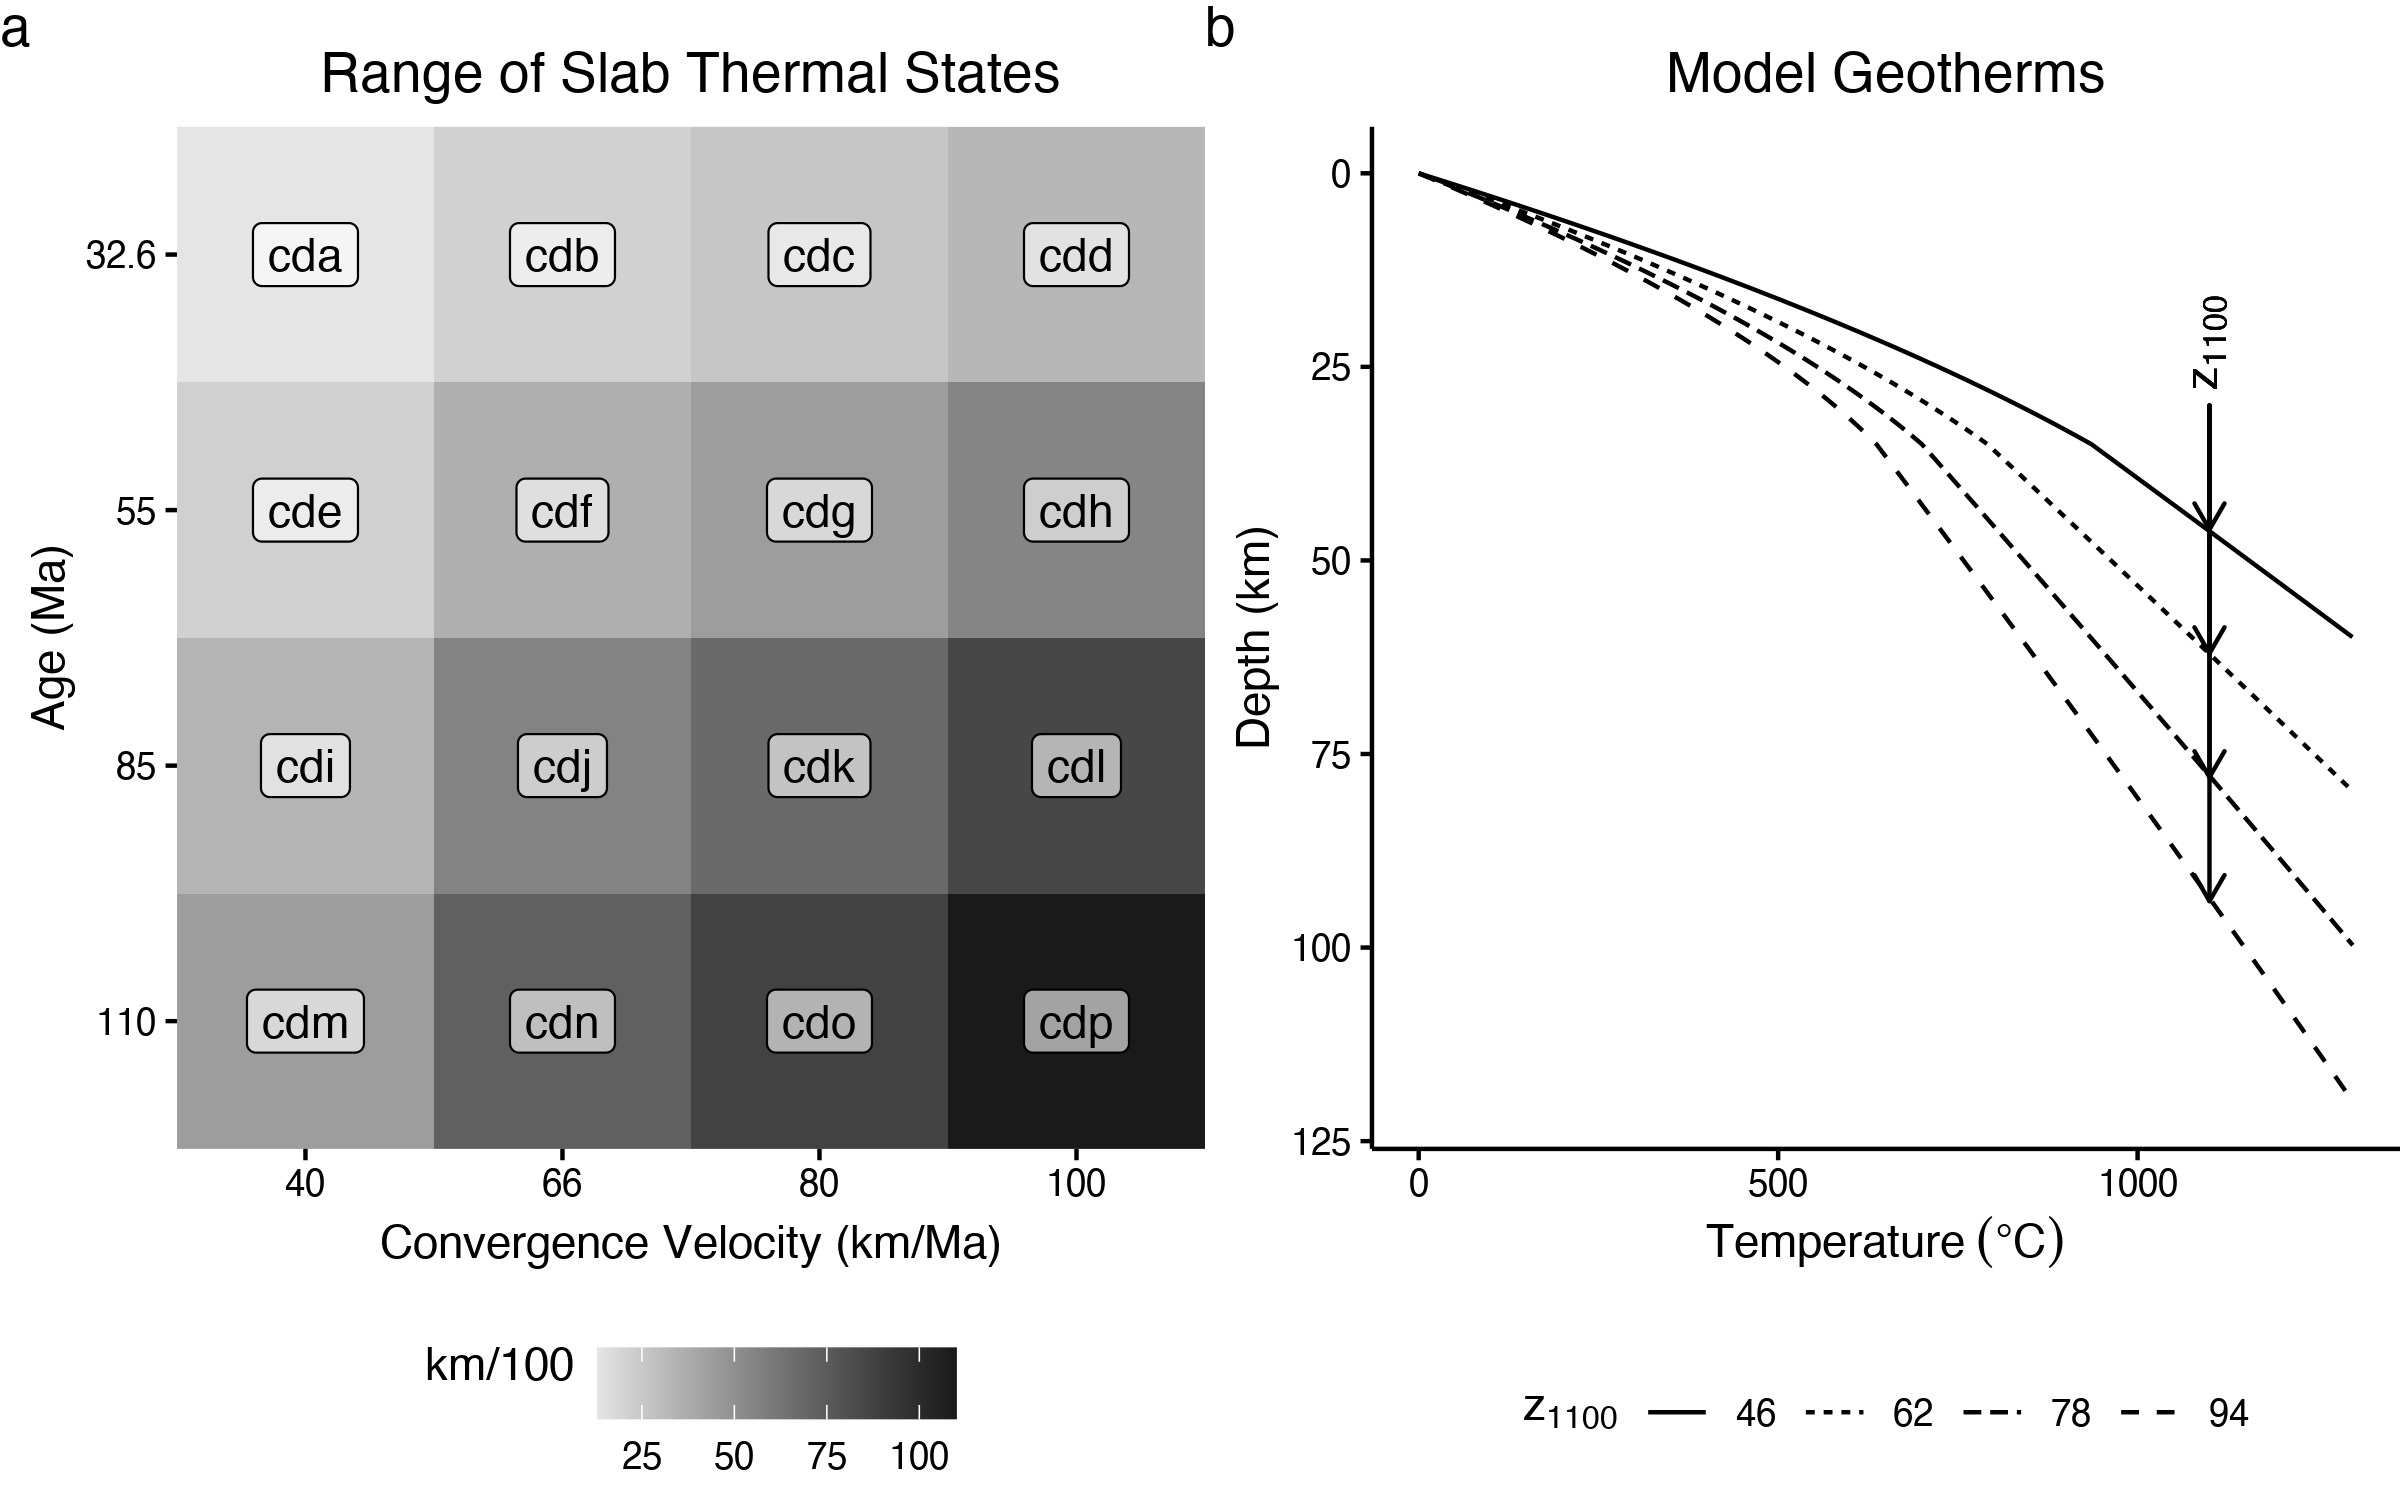
\includegraphics[width=1\linewidth,]{figs/fig2}

}

\caption{The range of key parameters investigated in this study. (a) Modelled thermal parameters range from 13 to 110 $km/100$ and broadly reflect the distribution of slab ages and convergence velocities in modern subduction zones. Model names include the prefix "cd" for "coupling depth" with increasing alphabetic suffixes. Note that neither axes are continuous. (b) Geotherms were constructed using a one-dimensional steady-state conductive cooling model using $T(z$=$0)$=$0\ ^{\circ}C$ and $q(z$=$0)$=$59,\ 63,\ 69,\ 79\ mW/m^{2}$, and constant radiogenic heating of 1.0 $\mu W/m^{3}$ for a 35 $km$-thick crust and 0.022 $\mu W/m^{3}$ for the mantle. The continental geotherms are calculated up to 1300 $^{\circ}$C, with a 0.5 $^{\circ}C/km$ gradient (the mantle adiabat) for higher temperatures.}\label{fig:params}
\end{figure}
\DIFaddend

\DIFaddbegin \begin{table}

\caption{\label{tab:melts}Melting curves used in numerical experiments}
\centering
\resizebox{\linewidth}{!}{
\begin{threeparttable}
\begin{tabular}[t]{lrrlrlrrrrr}
\toprule
\multicolumn{1}{c}{} & \multicolumn{8}{c}{Solidus Constants$^1$} & \multicolumn{2}{c}{Liq Constants$^2$} \\
\cmidrule(l{3pt}r{3pt}){2-9} \cmidrule(l{3pt}r{3pt}){10-11}
Material & $a$ & $b$ & $c$ & $d$ & $e$ & $f$ & $g$ & $h$ & $i$ & $j$\\
\midrule
\cellcolor{gray!6}{Felsic sediments} & \cellcolor{gray!6}{1200} & \cellcolor{gray!6}{889} & \cellcolor{gray!6}{1.79e+04} & \cellcolor{gray!6}{54} & \cellcolor{gray!6}{2.02e+04} & \cellcolor{gray!6}{831} & \cellcolor{gray!6}{6.00e-02} & \cellcolor{gray!6}{0} & \cellcolor{gray!6}{1262} & \cellcolor{gray!6}{0.009}\\
Felsic crust & 1200 & 889 & 1.79e+04 & 54 & 2.02e+04 & 831 & 6.00e-02 & 0 & 1262 & 0.009\\
\cellcolor{gray!6}{Oceanic Crust} & \cellcolor{gray!6}{1600} & \cellcolor{gray!6}{973} & \cellcolor{gray!6}{7.04e+05} & \cellcolor{gray!6}{354} & \cellcolor{gray!6}{7.78e+07} & \cellcolor{gray!6}{935} & \cellcolor{gray!6}{3.50e-03} & \cellcolor{gray!6}{62} & \cellcolor{gray!6}{1423} & \cellcolor{gray!6}{0.105}\\
Dry mantle & 0 & 0 & 0 & 0 & 0 & 1394 & 1.33e-01 & -51 & 2073 & 0.114\\
\cellcolor{gray!6}{Hydrated mantle} & \cellcolor{gray!6}{2400} & \cellcolor{gray!6}{1240} & \cellcolor{gray!6}{4.98e+04} & \cellcolor{gray!6}{323} & \cellcolor{gray!6}{0} & \cellcolor{gray!6}{0} & \cellcolor{gray!6}{1.27e+05} & \cellcolor{gray!6}{35} & \cellcolor{gray!6}{2073} & \cellcolor{gray!6}{0.114}\\
\addlinespace
Serpentinized mantle & 2400 & 1240 & 4.98e+04 & 323 & 0 & 0 & 1.27e+05 & 35 & 2073 & 0.114\\
\bottomrule
\end{tabular}
\begin{tablenotes}
\item After phase diagrams from Schmidt \& Poli (1998)
\item[\DIFaddFL{1}] $T(Solidus)=b+\frac{c}{(P+d)}+\frac{e}{(P+d)^2}$ at $P<a$, $f+gP+hP^2$ at $P\geq a$, $P$ in $[MPa]$, $T$ in $[K]$
\item[\DIFaddFL{2}] $T(Liquidus) = i+jP$, $P$ in $[MPa]$, $T$ in $[K]$
\end{tablenotes}
\end{threeparttable}}
\end{table}

\DIFaddend \subsection{Calculating geotherms and defining lithospheric thickness}
\DIFaddbegin

\DIFaddend The oceanic crust was modeled as 1 \DIFdelbegin \DIFdel{$km$ }\DIFdelend \DIFaddbegin \DIFadd{\(km\) }\DIFaddend of sediment cover overlying 2
\DIFdelbegin \DIFdel{$km$ }\DIFdelend \DIFaddbegin \DIFadd{\(km\) }\DIFaddend of basalt and 5 \DIFdelbegin \DIFdel{$km$ }\DIFdelend \DIFaddbegin \DIFadd{\(km\) }\DIFaddend of gabbro (\DIFdelbegin \DIFdel{Fig.~\ref{Figure1}b}\DIFdelend \DIFaddbegin \DIFadd{Figure~\ref{fig:init}a}\DIFaddend ).
Oceanic lithosphere was continually made at a pseudo-mid-ocean ridge on
the left boundary of the model \DIFaddbegin \DIFadd{(Figure~\ref{fig:init}b) }\DIFaddend and an enhanced
vertical cooling condition was applied at 200 \DIFdelbegin \DIFdel{$km$ }\DIFdelend \DIFaddbegin \DIFadd{\(km\) }\DIFaddend from the mid-ocean
ridge to adjust for the proper oceanic plate age, and therefore its
lithospheric thickness as it enters the trench \DIFdelbegin %DIFDELCMD < \cite<Fig.~\ref{Figure1}c;>{Agrusta2013}%%%
\DIFdel{.}\DIFdelend \DIFaddbegin \DIFadd{(Agrusta et al., 2013).
}\DIFaddend We used plate ages from 32.6 to 110 \DIFdelbegin \DIFdel{$Ma$ }\DIFdelend \DIFaddbegin \DIFadd{\(Ma\) }\DIFaddend and convergence velocities
from 40 to 100 \DIFdelbegin \DIFdel{$km/Ma$ (Fig.~\ref{Figure2}}\DIFdelend \DIFaddbegin \DIFadd{\(km/Ma\) (Figure~\ref{fig:params}}\DIFaddend a). This range of slab
parameters broadly reflects the middle-range of the modern global
subduction system \DIFdelbegin %DIFDELCMD < \cite{Syracuse2006}%%%
\DIFdelend \DIFaddbegin \DIFadd{(Syracuse \& Abers, 2006)}\DIFaddend .

The initial continental geotherms were determined by solving the heat
flow equation in one-dimension to 1300 \DIFdelbegin \DIFdel{$^{\circ}C$ (Fig.~\ref{Figure2}}\DIFdelend \DIFaddbegin \DIFadd{\(^{\circ}C\)
(Figure~\ref{fig:params}}\DIFaddend b). We assumed a fixed temperature of 0
\DIFdelbegin \DIFdel{$^{\circ}C$ }\DIFdelend \DIFaddbegin \DIFadd{\(^{\circ}C\) }\DIFaddend at the surface, constant radiogenic heating of 1
\DIFdelbegin \DIFdel{$\mu W/m^3$ }\DIFdelend \DIFaddbegin \DIFadd{\(\mu W/m^{3}\) }\DIFaddend in the 35 \DIFdelbegin \DIFdel{$km$}\DIFdelend \DIFaddbegin \DIFadd{\(km\)}\DIFaddend -thick continental crust and 0.022
\DIFdelbegin \DIFdel{$\mu W/m^3$ }\DIFdelend \DIFaddbegin \DIFadd{\(\mu W/m^{3}\) }\DIFaddend in the mantle, and thermal conductivities of 2.3
\DIFdelbegin \DIFdel{$W/mK$ }\DIFdelend \DIFaddbegin \DIFadd{\(W/mK\) }\DIFaddend and 3.0 \DIFdelbegin \DIFdel{$W/mK$ }\DIFdelend \DIFaddbegin \DIFadd{\(W/mK\) }\DIFaddend for the continental crust and mantle,
respectively. \DIFdelbegin \DIFdel{Below the }\DIFdelend \DIFaddbegin \DIFadd{Above, }\DIFaddend 1300 \DIFdelbegin \DIFdel{$^{\circ}C$ isotherm the temperature increases }\DIFdelend \DIFaddbegin \DIFadd{\(^{\circ}C\), temperature was assumed to
increase }\DIFaddend by 0.5 \DIFdelbegin \DIFdel{$^{\circ}C/km$ }\DIFdelend \DIFaddbegin \DIFadd{\(^{\circ}C/km\) }\DIFaddend (the mantle adiabat).

Many studies define the base of the continental lithosphere at the 1300
\DIFdelbegin \DIFdel{$^{\circ}C$ }\DIFdelend \DIFaddbegin \DIFadd{\(^{\circ}C\) }\DIFaddend isotherm, but it can be determined more accurately from
viscosity and strain rate as the model progresses. The mechanical base
of the lithosphere in our models generally occurred around the 1100
\DIFdelbegin \DIFdel{$^{\circ}C$ isotherm\textemdash characterized }\DIFdelend \DIFaddbegin \DIFadd{\(^{\circ}C\) isotherm---characterized }\DIFaddend by a rapid decrease in viscosity
and increase in strain rate
\DIFaddbegin \DIFadd{(Figures~\ref{fig:cdfstep1}, \ref{fig:cdfstep2}, \ref{fig:cdfstep3})}\DIFaddend . As
such, we consider the oceanic and continental lithosphere in this study
as mechanical layers \DIFaddbegin \DIFadd{defined by viscosity, rather than merely
temperature}\DIFaddend . For convenience, we refer to the continental lithospheric
thickness as \DIFdelbegin \DIFdel{$z_{1100}$ because its }\DIFdelend \DIFaddbegin \DIFadd{\(z_{1100}\) because of its general }\DIFaddend correspondence with the
1100 \DIFdelbegin \DIFdel{$^{\circ}C$ isothermmakes it discernable in figures where we draw isotherms, but do not explicitly visualize viscosity or strain rate. To match our }\DIFdelend \DIFaddbegin \DIFadd{\(^{\circ}C\) isotherm. Our }\DIFaddend modelled range of \DIFdelbegin \DIFdel{backarc heat flow}\DIFdelend \DIFaddbegin \DIFadd{\(z_{1100}\)
corresponds to backarc surface heat flow of 59, 63}\DIFaddend , \DIFdelbegin \DIFdel{$z_{1100}$ ranged from 46 to 94 $km$ (Fig.
~\ref{Figure2}b).
}\DIFdelend \DIFaddbegin \DIFadd{69, and 79
\(mW/m^{2}\).
}\DIFaddend

\subsection{Metamorphic (de)hydration reactions}
\DIFaddbegin

\DIFaddend Our use of Lagrangian markers to store pressure, temperature, and
rheology \DIFdelbegin \DIFdel{corresponding with rock-specific flow laws allows for changes to material properties (e.g., viscosity, density, etc.) that can result from }\DIFdelend \DIFaddbegin \DIFadd{allows for subsequent changes of material properties for rocks
undergoing simulated }\DIFaddend metamorphic reactions. In our models, we focused on
dehydration reactions in the slab and the formation and breakdown of
antigorite in the mantle wedge. For computational efficiency our models
did not solve for thermodynamically stable mineral assemblages to
compute water contents for the slab and mantle wedge \DIFdelbegin %DIFDELCMD < \cite<e.g.,>[]{Connolly2005}%%%
\DIFdel{.Instead, for the slab,
}\DIFdelend \DIFaddbegin \DIFadd{(e.g., Connolly,
2005). Instead, }\DIFaddend we implemented a simple model for gradual dehydration
(eclogitization) of \DIFdelbegin \DIFdel{the crust}\DIFdelend \DIFaddbegin \DIFadd{oceanic crust, }\DIFaddend computed as a linear function of
depth (lithostatic pressure)\DIFaddbegin \DIFadd{, }\DIFaddend with a maximum depth (150 \DIFdelbegin \DIFdel{$km$}\DIFdelend \DIFaddbegin \DIFadd{\(km\)}\DIFaddend ) where
the slab was completely dehydrated. This approach effectively simulates
a continuous influx of water to the mantle wedge, beginning with
compaction and release of connate water at shallow depths, followed by a
sequence of reactions consuming major hydrous phases (chlorite,
lawsonite, zoisite, chloritoid, talc, amphibole, and phengite) in
different parts of the hydrated basaltic crust \DIFdelbegin %DIFDELCMD < \cite{Schmidt1998}%%%
\DIFdel{.}\DIFdelend \DIFaddbegin \DIFadd{(Schmidt \& Poli, 1998;
van Keken et al., 2011). We implicitly assume slabs of different ages
release water similarly. Older slabs, however, should carry water to
greater depths because water-releasing reactions will be delayed along
cold subduction thermal gradients, relative to younger slabs with warmer
subduction thermal gradients (Peacock, 1996).
}\DIFaddend

For the mantle wedge, hydration of strong peridotite to form weak
brucite and serpentine along the subduction interface is likely
responsible for mechanical decoupling between the slab and the mantle
wedge at shallow levels \DIFdelbegin %DIFDELCMD < \cite{Peacock1999a, Hyndman2003}%%%
\DIFdelend \DIFaddbegin \DIFadd{(Hyndman \& Peacock, 2003; Peacock \& Hyndman,
1999)}\DIFaddend . If so, noting that brucite breaks down at much lower temperatures
than serpentine \DIFdelbegin %DIFDELCMD < \cite{Schmidt1998}%%%
\DIFdel{, }\DIFdelend \DIFaddbegin \DIFadd{(Schmidt \& Poli, 1998), }\DIFaddend the loss of serpentine likely
represents the key transition from a weak wedge (and subduction
interface) to a strong wedge. Dehydration of serpentine was modelled as
an abrupt, discontinuous reaction, which is a good approximation for
\DIFdelbegin \DIFdel{extremely }\DIFdelend \DIFaddbegin \DIFadd{near-endmember compositions, like (}\DIFaddend Mg-rich\DIFdelbegin \DIFdel{rocks like }\DIFdelend \DIFaddbegin \DIFadd{) }\DIFaddend peridotites. The P-T
conditions of the reaction
\DIFdelbegin \DIFdel{$antigorite \Leftrightarrow olivine + orthopyroxene + H_{2}O$ }\DIFdelend \DIFaddbegin \DIFadd{\(antigorite \Leftrightarrow olivine + orthopyroxene + H_{2}O\) }\DIFaddend were
based on the experimentally determined stability field from \DIFdelbegin %DIFDELCMD < \citet{Schmidt1998} %%%
\DIFdelend \DIFaddbegin \DIFadd{Schmidt \&
Poli (1998) }\DIFaddend and implemented into our model using the following equation:

\DIFdelbegin %DIFDELCMD < \begin{equation}
%DIFDELCMD <  \begin{alignedat}{2}
%DIFDELCMD <   T_{atg-out}(z) &= 751.50+\num{6.008d-3}z-\num{3.469d-8}z^2, && \text{for $z<63000m$} \\
%DIFDELCMD <   T_{atg-out}(z) &= 1013.2-\num{6.039d-5}z-\num{4.289d-9}z^2, && \text{for $z>63000m$}
%DIFDELCMD <  \end{equation}%%%
\DIFdelend \DIFaddbegin \begin{equation}\protect\hypertarget{eq:antstab}{}{\begin{aligned}
  T_{atg-out}(z) &= 751.50+6.008\times10^{-3}z-3.469\times10^{-8}z^2 & & for~z<63000m \\
  T_{atg-out}(z) &= 1013.2-6.039\times10^{-5}z-4.289\times10{-9}z^2 & & for~z>63000m
 \end{aligned}}\label{eq:antstab}\end{equation}\DIFaddend
\DIFdelbegin %DIFDELCMD < \label{Equation1}
%DIFDELCMD < \end{alignedat}
%DIFDELCMD < %%%
\DIFdelend

where \DIFdelbegin \DIFdel{$z$ }\DIFdelend \DIFaddbegin \DIFadd{\(z\) }\DIFaddend is the depth of a marker from the surface in meters and
\DIFdelbegin \DIFdel{$T$ }\DIFdelend \DIFaddbegin \DIFadd{\(T\) }\DIFaddend is temperature in Kelvins. This reaction placement is also
consistent to within 25 \DIFdelbegin \DIFdel{$^{\circ}C$ }\DIFdelend \DIFaddbegin \DIFadd{\(^{\circ}C\) }\DIFaddend with recent experiments \DIFdelbegin %DIFDELCMD < \cite{Shen2015}%%%
\DIFdel{.}\DIFdelend \DIFaddbegin \DIFadd{(Shen et
al., 2015). }\DIFaddend Under assumptions of thermodynamic equilibrium, markers
whose internal temperature exceeds \DIFdelbegin \DIFdel{$T(z)$  spontaneously formed
$olivine \allowbreak+ orthopyroxene \allowbreak+ H_2O$}\DIFdelend \DIFaddbegin \DIFadd{\(T(z)\) spontaneously formed
\(olivine + orthopyroxene + H_{2}O\)}\DIFaddend , releasing their crystal-bound
water. \DIFaddbegin \DIFadd{This implementation is common to versions of I2VIS that do not
implement thermodynamic computations of mineral stability (e.g.,
Connolly, 2005).
}\DIFaddend

The excess water released by a rock marker was modelled as a fluid
particle that migrates through \DIFaddbegin \DIFadd{moving }\DIFaddend rocks with a \DIFaddbegin \DIFadd{relative }\DIFaddend velocity
defined by \DIFdelbegin \DIFdel{pressure gradients }%DIFDELCMD < \cite[see Appendix A]{Faccenda2009}%%%
\DIFdel{.}\DIFdelend \DIFaddbegin \DIFadd{local pressure gradients, scaled by a 10 \(cm/yr\) vertical
percolation velocity corresponding to a purely lithostatic pressure
gradient in the mantle (see Appendix, Faccenda et al., 2009). }\DIFaddend The fluid
particle migrates until it reaches material that can consume an
additional amount of water by equilibrium hydration reactions (e.g.,
\DIFdelbegin \DIFdel{equation~\ref{Equation1}}\DIFdelend \DIFaddbegin \DIFadd{Equation~\ref{eq:antstab}}\DIFaddend ). Theoretically, the mantle can store large
amounts of water because antigorite is stable at shallow mantle
conditions and can contain up to 13 \DIFdelbegin \DIFdel{$wt.\%$ water }%DIFDELCMD < \cite{Reynard2013}%%%
\DIFdelend \DIFaddbegin \DIFadd{\(wt.\%\) water (Reynard, 2013)}\DIFaddend .
Thermodynamic models predict 8 \DIFdelbegin \DIFdel{$wt.\%$ }\DIFdelend \DIFaddbegin \DIFadd{\(wt.\%\) }\DIFaddend water in the mantle wedge
\DIFdelbegin %DIFDELCMD < \cite{Connolly2005}%%%
\DIFdelend \DIFaddbegin \DIFadd{(Connolly, 2005)}\DIFaddend . However, seismic studies suggest that most forearcs
are only partially serpentinized (\DIFdelbegin \DIFdel{$<$ }\DIFdelend \DIFaddbegin \DIFadd{\(<\) }\DIFaddend 20-40 \DIFdelbegin \DIFdel{$\%$}\DIFdelend \DIFaddbegin \DIFadd{\(\%\)}\DIFaddend ), equating to water
contents of ca. 3-6 \DIFdelbegin \DIFdel{$wt.\%$ }%DIFDELCMD < \cite{Abers2017, Carlson2003}%%%
\DIFdel{.}\DIFdelend \DIFaddbegin \DIFadd{\(wt.\%\) (Abers et al., 2017; Carlson \& Miller,
2003). }\DIFaddend Therefore we limit mantle wedge hydration to \DIFdelbegin \DIFdel{$\leq$ }\DIFdelend \DIFaddbegin \DIFadd{\(\leq\) }\DIFaddend 2
\DIFdelbegin \DIFdel{$wt.\% ~H_2O$ }\DIFdelend \DIFaddbegin \DIFadd{\(wt.\%\ H_{2}O\) }\DIFaddend and assume any \DIFdelbegin \DIFdel{$H_2O$ }\DIFdelend \DIFaddbegin \DIFadd{\(H_{2}O\) }\DIFaddend in excess exits the system
through channelized fluid flow \DIFdelbegin %DIFDELCMD < \cite{Davies1999}%%%
\DIFdelend \DIFaddbegin \DIFadd{(Davies, 1999)}\DIFaddend .

\subsection{\DIFdelbegin \DIFdel{Calculating surface heat flow}\DIFdelend \DIFaddbegin \DIFadd{Rheologic Model}\DIFaddend }
\DIFdelbegin \DIFdel{We calculated vertical heat flux based on the temperature difference between the 2 $km$ deep node and the next lower node, their separation distance, }\DIFdelend \DIFaddbegin

\DIFadd{Contributions from dislocation and diffusion creep flow laws are taken
into account by computing a composite rheology for ductile rocks,
\(\eta_{creep}\):
}

\begin{equation}\protect\hypertarget{eq:ductile}{}{\begin{aligned}\frac{1}{\eta_{creep}} = \frac{1}{\eta_{diff}} + \frac{1}{\eta_{disl}}\end{aligned}}\label{eq:ductile}\end{equation}

\DIFadd{\(\eta_{diff}\) }\DIFaddend and \DIFdelbegin \DIFdel{the average thermal conductivity between them. We calculated heat flux at 2 $km$ depth rather than at the surface to avoid numerical errors}\DIFdelend \DIFaddbegin \DIFadd{\(\eta_{disl}\) are effective viscosities for
diffusion and dislocation creep, respectively.
}

\DIFadd{For the crust and serpentinized mantle, \(\eta_{diff}\) and
\(\eta_{disl}\) are computed as:
}

\begin{equation}\protect\hypertarget{eq:crust}{}{\begin{aligned}\eta_{diff} &= \frac{A}{2\sigma_{cr}^{n - 1}}\exp\left( \frac{E + PV}{RT} \right) \\\\
\eta_{disl} &= \frac{1}{2}A^{\frac{1}{n}}\exp\left( \frac{E + PV}{nRT} \right){\dot{\varepsilon}}_{II}^{\frac{1}{n} - 1}\end{aligned}}\label{eq:crust}\end{equation}

\DIFadd{where \(R\) is gas constant, \(P\) is pressure, \(T\) is temperature (in
\(K\)),
\({\dot{\varepsilon}}_{II} = \sqrt{1/2{({\dot{\varepsilon}}_{ij})}^{2}}\)
is the square root of the second invariant of the strain rate tensor,
\(\sigma_{cr}\) is the assumed diffusion-dislocation transition stress,
and \(A\), \(E\), \(V\) and \(n\) are the material constant, activation
energy, activation volume, and stress exponent, respectively (Table
\ref{tab:materials}, Hilairet et al., 2007; Ranalli, 1995).
}

\DIFadd{For the mantle, \(\eta_{diff}\) and \(\eta_{disl}\) are computed as
(Karato \& Wu, 1993):
}

\begin{equation}\protect\hypertarget{eq:mantle}{}{\begin{aligned}\eta_{diff} &= \frac{G}{2A_{diff}}\left( \frac{h}{b} \right)^{\frac{m}{n}}\exp\left( \frac{E_{diff} + PV_{diff}}{RT} \right) \\\\
\eta_{disl} &= \frac{G}{2A_{disl}^{\frac{1}{n}}}\exp\left( \frac{E_{disl} + PV_{disl}}{nRT} \right){\dot{\varepsilon}}_{II}^{\frac{1}{n} - 1}\end{aligned}}\label{eq:mantle}\end{equation}

\DIFadd{where \(b\)=\(5\times10^{-10}\) \(m\) is Burgers vector,
\(G\)=\(8\times10^{10}\) \(Pa\) is shear modulus, \(h\) is the assumed
grain size, \(m\) is the grain size exponent, and the other flow law
parameters are given in Table \ref{tab:materials}. Our models limited
viscosity for all rocks at \(\eta_{min} = 10^{17}\ Pa \cdot s\) and
\(\eta_{max} = 10^{25}\ Pa \cdot s\)}\DIFaddend .

\DIFaddbegin \DIFadd{The ductile rheology, \(\eta_{creep}\), is combined with a brittle
(plastic) rheology to yield an effective viscous-plastic rheology using
the following upper limit for the ductile viscosity:
}

\begin{equation}\protect\hypertarget{eq:plastic}{}{\begin{aligned}\eta_{creep}\ \  &\leq \frac{C + \mu P}{2{\dot{\varepsilon}}_{II}} \\
\mu\  &= \ \mu_{0} - \gamma\mu_{\gamma} & & for~~\gamma \leq \gamma_0 0 \\
\mu &= \mu_1 & & for~~\gamma > \gamma_0 \\
\gamma &= \int_{}^{}\sqrt{\frac{1}{2}{({\dot{\varepsilon}}_{ij(plastic)})}^{2}}dt\end{aligned}}\label{eq:plastic}\end{equation}

\DIFadd{where \(\mu\) is the internal friction coefficient, (\(\mu_0\) and
\(\mu_1\) are the initial and final internal friction coefficients,
respectively, Table \ref{tab:materials}),
\(\mu_\gamma = (\mu_0 - \mu_1)/\gamma_0\) is the fault weakening rate
with integrated plastic strain, \(\gamma\) (\(\gamma_0\)=1 is the upper
strain limit for fracture-related weakening), \(C\) is the rock
compressive strength at \(P\)=0 (Table \ref{tab:materials}), \(t\) is
time (\(s\)), and \({\dot{\varepsilon}}_{ij(plastic)}\) is the plastic
strain rate tensor.
}

\DIFaddend \subsection{Visualization and determination of coupling depth}
\DIFaddbegin

\DIFaddend For each run (e.g., \DIFdelbegin \DIFdel{Fig.~\ref{Figure3}}\DIFdelend \DIFaddbegin \DIFadd{Figure~\ref{fig:comp}}\DIFaddend ) we made calculations at
\DIFdelbegin \DIFdel{$\sim$}\DIFdelend \DIFaddbegin \DIFadd{\(\sim\) }\DIFaddend 10 \DIFdelbegin \DIFdel{$Ma$ }\DIFdelend \DIFaddbegin \DIFadd{\(Ma\) }\DIFaddend for surface heat flow (\DIFdelbegin \DIFdel{Fig.~\ref{Figure3}a)and visualized }\DIFdelend \DIFaddbegin \DIFadd{Figure~\ref{fig:comp}a), }\DIFaddend rock
type (\DIFdelbegin \DIFdel{Fig.~\ref{Figure3}}\DIFdelend \DIFaddbegin \DIFadd{Figure~\ref{fig:comp}}\DIFaddend b, c), temperature (\DIFdelbegin \DIFdel{Fig.~\ref{Figure3}}\DIFdelend \DIFaddbegin \DIFadd{Figure~\ref{fig:comp}}\DIFaddend d),
viscosity (\DIFdelbegin \DIFdel{Fig.~\ref{Figure3}}\DIFdelend \DIFaddbegin \DIFadd{Figure~\ref{fig:comp}}\DIFaddend e), strain rate
(\DIFdelbegin \DIFdel{Fig.~\ref{Figure3}}\DIFdelend \DIFaddbegin \DIFadd{Figure~\ref{fig:comp}}\DIFaddend f), \DIFdelbegin \DIFdel{and an effective P\'{e}clet number (detailed below}\DIFdelend \DIFaddbegin \DIFadd{shear heating (Figure~\ref{fig:comp}g), and
flow velocity (Figure~\ref{fig:comp}h}\DIFaddend ). We chose 10 \DIFdelbegin \DIFdel{$Ma$ }\DIFdelend \DIFaddbegin \DIFadd{\(Ma\) }\DIFaddend because
changes to the overall dynamics and thermal structure are small after
ca. 5 \DIFdelbegin \DIFdel{$Ma$ }\DIFdelend \DIFaddbegin \DIFadd{\(Ma\) }\DIFaddend and the additional 5 \DIFdelbegin \DIFdel{$Ma$ }\DIFdelend \DIFaddbegin \DIFadd{\(Ma\) }\DIFaddend provides sufficient time for
the geodynamics to \DIFdelbegin \DIFdel{fully stabilize (see
Fig.~\ref{FigureS1}}\DIFdelend \DIFaddbegin \DIFadd{reach quasi-steady state (see
Figure~\ref{fig:antdepth}}\DIFaddend ).

\DIFdelbegin %DIFDELCMD < \begin{center}
%DIFDELCMD <  
\includegraphics[width=\textwidth, trim={0 0 0 0}]{figs/Fig3.png}
%DIFDELCMD <  \label{Figure3}
%DIFDELCMD <  \captionof{figure}{Visualization of model cdf with a 78 $km$-thick backarc lithosphere at $\sim$10 $Ma$. Arc positions are marked by triangles. (a) Surface heat flow calculated at a depth of 2 $km$ beneath the surface(see text for explanation). (b) Rock type for the entire model domain. (c) Rock type in the region from the trench to approximately 220 $km$ into the backarc. By 10 $Ma$ a serpentine channel has formed, entraining material from the top of the down-going slab and lubricating the interface between slab and mantle. (d) Temperature distribution. (e) Log viscosity. The viscosity contrast between the slab and serpentinized mantle in the forearc effectively decouples the slab and mantle wedge mechanically, but abruptly diminishes as the principally weak material (antigorite) is removed by reaction. (f) Log strain rate. In the shallow forearc, strain is localized in the weak serpentine channel. At the antigorite-out reaction, strain localization jumps towards the warm core of the mantle wedge. Circulation in the mantle wedge is restricted to beneath the stiff lithosphere. (g) Effective P\'{e}clet number. An effective P\'{e}clet number is the ratio of advective:conductive heat transport, scaled to the local thermal gradients (see text for formulation). “Cooler” colors (blues) vs. “warmer” colors (reds) indicate advection up vs. down the thermal gradient, i.e., high values show advection in the same direction as diffusion. An absolute value between 0 and ~10 (green) indicates much greater efficiency of heat transfer via thermal diffusion than via advection, whereas absolute values greater than ~40 (blues and reds) indicate high efficiency of heat transfer via advection \textit{and/or} a small local thermal gradient. Note the narrow region of dark red streaming towards the coupling point, indicating high efficiency of heat advection into the coupling region.}
%DIFDELCMD < \end{center}
%DIFDELCMD <

%DIFDELCMD < %%%
\DIFdelend We determined the mechanical coupling depth\DIFdelbegin \DIFdel{($z_c$) }\DIFdelend \DIFaddbegin \DIFadd{, \(z_{c}\), }\DIFaddend by visualizing
viscosity at \DIFdelbegin \DIFdel{$\sim$}\DIFdelend \DIFaddbegin \DIFadd{\(\sim\) }\DIFaddend 10 \DIFdelbegin \DIFdel{$Ma$ }\DIFdelend \DIFaddbegin \DIFadd{\(Ma\) }\DIFaddend and selecting a node closest to the
point where the viscosity contrast between the serpentinized- and
non-serpentinized basal mantle wedge diminishes to \DIFdelbegin \DIFdel{$<$ }\DIFdelend \DIFaddbegin \DIFadd{\(<\) }\DIFaddend 10\DIFdelbegin \DIFdel{$^2$ $Pa\cdot s$ (Fig.~}%DIFDELCMD < \allowbreak%%%
\DIFdel{\ref{Figure3}}\DIFdelend \DIFaddbegin \DIFadd{\(^{2}\)
\(Pa \cdot s\) (Figure~\ref{fig:comp}}\DIFaddend e). In this study we assume that
the mechanical coupling depth occurs instantaneously and at a single
node. However, mechanical coupling in reality must be dispersed across a
finite length along the slab-mantle interface. At the resolution of our
models, there was a small area (ca. 5x5 \DIFdelbegin \DIFdel{$km$ }\DIFdelend \DIFaddbegin \DIFadd{\(km\) }\DIFaddend or 5x5 nodes) where
\DIFdelbegin \DIFdel{$z_c$ }\DIFdelend \DIFaddbegin \DIFadd{\(z_{c}\) }\DIFaddend could appropriately be determined, giving an uncertainty in
our \DIFdelbegin \DIFdel{$z_c$ }\DIFdelend \DIFaddbegin \DIFadd{\(z_{c}\) }\DIFaddend determination on the order of \DIFdelbegin \DIFdel{$\pm$ }\DIFdelend \DIFaddbegin \DIFadd{\(\pm\) }\DIFaddend 2.5 \DIFdelbegin \DIFdel{$km$}\DIFdelend \DIFaddbegin \DIFadd{\(km\)}\DIFaddend .

\DIFdelbegin \subsection{\DIFdel{Formulation of an effective P\'{e}clet number}}
%DIFAUXCMD
\addtocounter{subsection}{-1}%DIFAUXCMD
\DIFdel{We calculated what we call the “effective P\'{e}clet number” to visualize and evaluate potential thermal feedbacks affecting the stability of antigorite in the mantle wedge. In its normal formulation, the P\'{e}clet number is a dimensionless number used to visualize the relative magnitude of (potential) heat transfer via advection vs. diffusion in a continuum }%DIFDELCMD < \cite{Patankar2018}%%%
\DIFdel{:
}\DIFdelend \DIFaddbegin \begin{figure}[h]

{\centering 
\includegraphics[width=1\linewidth,]{figs/fig3}

}

\caption{Visualization of model cdf with a 78 $km$-thick backarc lithosphere at $\sim$ 10 $Ma$. (a) Surface heat flow calculated at a depth of 2 $km$ beneath the surface. (b) Rock type for the entire model domain. (c) Rock type in the region from the trench to approximately 220 $km$ into the backarc shows a serpentine layer (pink) lubricating the interface between slab and mantle by 10 $Ma$. Melt is inconspicuous in the arc region because of low melt volumes and quick extraction. The effects of melting are more apparent in viscosity (e) and strain rate (f). (d) Temperature distribution shows strong thermal gradients ("bunching") near the coupling point where serpentine becomes unstable. (e) Log viscosity shows high contrast between the slab and serpentinized mantle in the forearc and low contrast where serpentine becomes unstable. Subvertical structure above coupling point reflects melt migration. (f) Log strain rate shows localized strain in the serpentine layer that expands towards the warm core of the mantle wedge as serpentine becomes unstable. Deformation in the mantle wedge is restricted to beneath the stiff lithosphere and along subvertical melt conduits. (g) Shear heating parallels strain rate and is focused into weakest horizons. (h) Streamlines show focused mantle wedge flow towards the coupling region. Rock type key is given in Table 3.}\label{fig:comp}
\end{figure}
\DIFaddend

\DIFdelbegin %DIFDELCMD < \begin{equation}
%DIFDELCMD <  \begin{gathered}
%DIFDELCMD <   Pe=\frac{advective~transport~rate}{diffusive~transport~rate} \\
%DIFDELCMD <   Pe=\frac{Lv}{\alpha} \\
%DIFDELCMD <   \alpha=\frac{\kappa}{\rho c_p}
%DIFDELCMD <  \end{gathered}
%DIFDELCMD <  \label{Equation3}
%DIFDELCMD < \end{equation}
%DIFDELCMD < %%%
\DIFdelend \DIFaddbegin \clearpage
\DIFaddend

\DIFdelbegin \DIFdel{where $L$ is a characteristic length, $v$ is the local velocity of the continuum, $\alpha$ is thermal diffusivity (or thermal diffusion coefficient), $\kappa$ is thermal conductivity, $\rho$ is the density, and $c_p$ is specific heat capacity.
}%DIFDELCMD <

%DIFDELCMD < %%%
\DIFdel{It is important to recognize that equation~\ref{Equation3} makes no explicit reference to the direction of heat transport. In particular, while heat always conducts down the (maximum) temperature gradient, i.e., perpendicular to isotherms and from high temperature to low temperature, advection may occur in any direction. Thus, depending on flow paths, advection could (a) augment local heat transport (a component of flow is parallel to and in the same direction as diffusion), (b) retard local heat transport (a component of flow is parallel to but in the opposite direction as diffusion) or (c) have no effect on local heat transport (flow is parallel to isotherms).
}%DIFDELCMD <

%DIFDELCMD < %%%
\DIFdel{In regions of complex flow dynamics and thermal structure, the standard formulation of the P\'{e}clet number can lead to implausible interpretations. For example, below the coupling depth, the base of the mantle wedge cools and new lithosphere forms atop the slab, which is dragged down by slab motion (Fig.~\ref{Figure3}e, g). This region has a high P\'{e}clet number, as calculated by equation~\ref{Equation3}, because the local velocity is very high and the thermal diffusion coefficient is only moderate. This form of the P\'{e}clet number would imply that thermal advection dominates heat transport. However, the closely spaced isotherms (large temperature gradients) within the same region imply that thermal diffusion is highly effective at transporting heat (Fig.~\ref{Figure3}g), while flow paths are nearly parallel to isotherms, implying that advection is ineffective. In terms of the effectiveness of heat transport, diffusion strongly outweighs advection, so intuitively the P\'{e}clet number should be small, not large.
}%DIFDELCMD <

%DIFDELCMD < %%%
\DIFdel{To better characterize heat transfer, we scale the P\'{e}clet number to the local thermal gradients as follows:
}%DIFDELCMD <

%DIFDELCMD < \begin{equation}
%DIFDELCMD <  Pe=\frac{Lv\nabla T_v}{\alpha\nabla T_{max}}
%DIFDELCMD <  \label{Equation4}
%DIFDELCMD < \end{equation}
%DIFDELCMD <

%DIFDELCMD < %%%
\DIFdel{where $\nabla T_v$ is the local thermal gradient }%DIFDELCMD < \protect%%%
\textit{\DIFdel{in the direction of the local velocity field}}%DIFAUXCMD
\DIFdel{, and $\nabla T_{max}$ is the maximum local thermal gradient that defines the effectiveness of heat diffusion. This formulation gives a better sense of heat transfer in a system where thermal gradients and velocity fields are highly non-uniform and have high contrasts. For the characteristic length scale, $L$, we use the slab thermal parameter, which scales the expression to the convergence velocity of the slab and the slab age, conveniently yielding numbers between 0 and 100 in most models. The final expression becomes:
}%DIFDELCMD <

%DIFDELCMD < \begin{equation}
%DIFDELCMD <  Pe=\frac{\Phi v\nabla T_v}{\alpha\nabla T_{max}}
%DIFDELCMD <  \label{Equation5}
%DIFDELCMD < \end{equation}
%DIFDELCMD <

%DIFDELCMD < %%%
\DIFdel{Because the temperature gradient in the direction of local flow can be positive or negative, an effective P\'{e}clet number can be positive or negative, where negative values indicate that advection and diffusion operate in opposite directions.
}%DIFDELCMD <

%DIFDELCMD < %%%
\DIFdelend \section{Results}
\DIFaddbegin

\DIFaddend \subsection{Coupling depth predictors}
\DIFaddbegin

\DIFaddend Across all 64 numerical models (\DIFdelbegin \DIFdel{Fig.~\ref{Figure4}; Table
~\ref{Table3}}\DIFdelend \DIFaddbegin \DIFadd{Figure~\ref{fig:results}, Table
\ref{tab:zc.results}}\DIFaddend ) coupling depth correlates strongly, but not
linearly, with increasing backarc lithospheric thickness
(\DIFdelbegin \DIFdel{$z_{1100}$; Fig.~\ref{Figure5}}\DIFdelend \DIFaddbegin \DIFadd{Figure~\ref{fig:biv}}\DIFaddend a). This correlation is a key result of our
experiments. Slab thermal parameter alone does not correlate obviously
with coupling depth (\DIFdelbegin \DIFdel{Fig.~\ref{Figure5}}\DIFdelend \DIFaddbegin \DIFadd{Figure~\ref{fig:biv}}\DIFaddend b). \DIFdelbegin \DIFdel{We determined the best fit model by considering }\DIFdelend \DIFaddbegin \DIFadd{Considering }\DIFaddend standard least
squares regressions \DIFdelbegin \DIFdel{that include }\DIFdelend \DIFaddbegin \DIFadd{of }\DIFaddend all possible permutations of the variables
\DIFdelbegin \DIFdel{$z_{1100}$, $z_{1100}^2$, and $\Phi$ (Tables~\ref{TableS1} and \ref{TableS2})}\DIFdelend \DIFaddbegin \DIFadd{\(z_{1100}\), \(z_{1100}^{2}\), and \(\Phi\), the following equation
optimizes the number of parameters, p value, and \(R^{2}\)}\DIFaddend :

\DIFdelbegin %DIFDELCMD < \begin{equation}
%DIFDELCMD <  z_{coupling}\sim \num{4.95d-3}z_{1100}^2-\num{9.27d-2}\Phi+63.6
%DIFDELCMD <  \label{Equation6}
%DIFDELCMD < \end{equation}%%%
\DIFdelend \DIFaddbegin \begin{equation}\protect\hypertarget{eq:zc}{}{\begin{aligned}z_{c} = 4.95 \times 10^{- 3}z_{1100}^{2} - 9.27 \times 10^{- 2}\Phi + 63.6\end{aligned}}\label{eq:zc}\end{equation}\DIFaddend

where \DIFdelbegin \DIFdel{$z$ and $\Phi$ are in $km$.Equation~\ref{Equation6} }\DIFdelend \DIFaddbegin \DIFadd{\(z\) is in \(km\) and \(\Phi\) is in \(km/100\). Regression
results are provided in Tables \textbackslash ref\{tab:anova\} and
\textbackslash ref\{tab:reg.summary\} and show that alternative linear
and quadratic models of \(z_c\) vs.~\(z_{1100}\) and \(\Phi\) fit the
experiments well. Equation~\ref{eq:zc} }\DIFaddend permits the prediction of the
mechanical coupling depths in modern subduction zones where \DIFdelbegin \DIFdel{backarc lithospheric thickness (inverted from backarc heat flow ) and slab thermal parameter can be estimated.
A web-based application to perform such calculations is available for free online (see Appendix A)
}\DIFdelend \DIFaddbegin \DIFadd{\(z_{c}\)
can be inverted from heat flow and \(\Phi\) is estimated.
}\DIFaddend

\DIFdelbegin %DIFDELCMD < \begin{figure}
%DIFDELCMD <  \centering
%DIFDELCMD <  
\includegraphics[width=\textwidth, trim={0 0 0 0}]{figs/Fig4.png}
%DIFDELCMD <  \caption{Visualized table of coupling depth as determined across a range of lithospheric thicknesses and thermal parameters. Note that the thermal parameter axis is not linear. Corresponding experiment is listed along the top of the array. Coupling depth increases systematically with increasing backarc lithospheric thickness (change in grayscale down columns) for all models. Any trend in coupling depth with respect to slab thermal parameter (change in grayscale across rows) is not apparent.}
%DIFDELCMD <  \label{Figure4}
%DIFDELCMD < \end{figure}
%DIFDELCMD < %%%
\DIFdelend \DIFaddbegin \begin{figure}[h]

{\centering 
\includegraphics[width=1\linewidth,]{figs/fig4}

}

\caption{Visual table of coupling depth as determined across a range of lithospheric thicknesses and thermal parameters. Note that the thermal parameter axis is not linear. Corresponding experiments are listed along the top of the array. Coupling depth increases systematically with increasing backarc lithospheric thickness (change in grayscale down columns) for all models. Any trend in coupling depth with respect to slab thermal parameter (change in grayscale across rows) is less apparent.}\label{fig:results}
\end{figure}
\DIFaddend

\DIFdelbegin %DIFDELCMD < \begin{longtable}{A{0.13} B{0.12} B{0.12} B{0.10}}
%DIFDELCMD <  \caption{Experimental results}               \\
%DIFDELCMD <  \label{Table3}                               \\
%DIFDELCMD <  \toprule
%DIFDELCMD <

%DIFDELCMD <  Experiment & $z_{1100}$ & $\phi/100$ & $z_c$ \\
%DIFDELCMD <             & $km$       & $km/100$   & $km$  \\
%DIFDELCMD <

%DIFDELCMD <  \midrule
%DIFDELCMD <  \endfirsthead
%DIFDELCMD <

%DIFDELCMD <  \caption{Experimental results (cont.).}      \\
%DIFDELCMD <  \label{Table3}                               \\
%DIFDELCMD <  \toprule
%DIFDELCMD <

%DIFDELCMD <  Experiment & $z_{1100}$ & $\phi/100$ & $z_c$ \\
%DIFDELCMD <             & $km$       & $km/100$   & $km$  \\
%DIFDELCMD <

%DIFDELCMD <  \midrule
%DIFDELCMD <  \endhead
%DIFDELCMD <

%DIFDELCMD <  \midrule
%DIFDELCMD <  \multicolumn{4}{r}{\footnotesize Continued on the next page}
%DIFDELCMD <  \endfoot
%DIFDELCMD <  \bottomrule
%DIFDELCMD <  \endlastfoot
%DIFDELCMD <

%DIFDELCMD <  cda        & 46         & 13.0       & 66    \\
%DIFDELCMD <  cdb        & 46         & 21.5       & 74    \\
%DIFDELCMD <  cdc        & 46         & 26.1       & 69    \\
%DIFDELCMD <  cdd        & 46         & 32.6       & 67    \\
%DIFDELCMD <  cde        & 46         & 22.0       & 72    \\
%DIFDELCMD <  cdf        & 46         & 36.3       & 78    \\
%DIFDELCMD <  cdg        & 46         & 44.0       & 78    \\
%DIFDELCMD <  cdh        & 46         & 55.0       & 59    \\
%DIFDELCMD <  cdi        & 46         & 34.0       & 80    \\
%DIFDELCMD <  cdj        & 46         & 56.1       & 70    \\
%DIFDELCMD <  cdk        & 46         & 68.0       & 58    \\
%DIFDELCMD <  cdl        & 46         & 85.0       & 65    \\
%DIFDELCMD <  cdm        & 46         & 44.0       & 79    \\
%DIFDELCMD <  cdn        & 46         & 72.6       & 70    \\
%DIFDELCMD <  cdo        & 46         & 88.0       & 68    \\
%DIFDELCMD <  cdp        & 46         & 110        & 64    \\
%DIFDELCMD <  cda        & 62         & 13.0       & 80    \\
%DIFDELCMD <  cdb        & 62         & 21.5       & 79    \\
%DIFDELCMD <  cdc        & 62         & 26.1       & 78    \\
%DIFDELCMD <  cdd        & 62         & 32.6       & 77    \\
%DIFDELCMD <  cde        & 62         & 22.0       & 87    \\
%DIFDELCMD <  cdf        & 62         & 36.3       & 82    \\
%DIFDELCMD <  cdg        & 62         & 44.0       & 75    \\
%DIFDELCMD <  cdh        & 62         & 55.0       & 70    \\
%DIFDELCMD <  cdi        & 62         & 34.0       & 91    \\
%DIFDELCMD <  cdj        & 62         & 56.1       & 77    \\
%DIFDELCMD <  cdk        & 62         & 68.0       & 72    \\
%DIFDELCMD <  cdl        & 62         & 85.0       & 67    \\
%DIFDELCMD <  cdm        & 62         & 44.0       & 88    \\
%DIFDELCMD <  cdn        & 62         & 72.6       & 77    \\
%DIFDELCMD <  cdo        & 62         & 88.0       & 74    \\
%DIFDELCMD <  cdp        & 62         & 110        & 75    \\
%DIFDELCMD <  cda        & 78         & 13.0       & 87    \\
%DIFDELCMD <  cdb        & 78         & 21.5       & 94    \\
%DIFDELCMD <  cdc        & 78         & 26.1       & 97    \\
%DIFDELCMD <  cdd        & 78         & 32.6       & 97    \\
%DIFDELCMD <  cde        & 78         & 22.0       & 90    \\
%DIFDELCMD <  cdf        & 78         & 36.3       & 90    \\
%DIFDELCMD <  cdg        & 78         & 44.0       & 88    \\
%DIFDELCMD <  cdh        & 78         & 55.0       & 85    \\
%DIFDELCMD <  cdi        & 78         & 34.0       & 97    \\
%DIFDELCMD <  cdj        & 78         & 56.1       & 91    \\
%DIFDELCMD <  cdk        & 78         & 68.0       & 84    \\
%DIFDELCMD <  cdl        & 78         & 85.0       & 77    \\
%DIFDELCMD <  cdm        & 78         & 44.0       & 78    \\
%DIFDELCMD <  cdn        & 78         & 72.6       & 87    \\
%DIFDELCMD <  cdo        & 78         & 88.0       & 85    \\
%DIFDELCMD <  cdp        & 78         & 110        & 78    \\
%DIFDELCMD <  cda        & 94         & 13.0       & 95    \\
%DIFDELCMD <  cdb        & 94         & 21.5       & 101   \\
%DIFDELCMD <  cdc        & 94         & 26.1       & 108   \\
%DIFDELCMD <  cdd        & 94         & 32.6       & 113   \\
%DIFDELCMD <  cde        & 94         & 22.0       & 100   \\
%DIFDELCMD <  cdf        & 94         & 36.3       & 104   \\
%DIFDELCMD <  cdg        & 94         & 44.0       & 104   \\
%DIFDELCMD <  cdh        & 94         & 55.0       & 104   \\
%DIFDELCMD <  cdi        & 94         & 34.0       & 101   \\
%DIFDELCMD <  cdj        & 94         & 56.1       & 102   \\
%DIFDELCMD <  cdk        & 94         & 68.0       & 101   \\
%DIFDELCMD <  cdl        & 94         & 85.0       & 107   \\
%DIFDELCMD <  cdm        & 94         & 44.0       & 106   \\
%DIFDELCMD <  cdn        & 94         & 72.6       & 102   \\
%DIFDELCMD <  cdo        & 94         & 88.0       & 98    \\
%DIFDELCMD <  cdp        & 94         & 110        & 108   \\
%DIFDELCMD < \end{longtable}
%DIFDELCMD < \begin{tablenotes}
%DIFDELCMD <  \footnotesize
%DIFDELCMD <  \item [] $z_{1100}$=lithospheric thickness, $\phi$=thermal parameter, $z_c$=coupling depth
%DIFDELCMD < \end{tablenotes}
%DIFDELCMD < %%%
\DIFdelend \DIFaddbegin \begin{landscape}\begin{table}
\caption{\label{tab:zc.results}Numerical modelling results}

\centering
\fontsize{8}{10}\selectfont
\begin{tabular}[t]{lrrr}
\toprule
Model & $z_{1100}$ & $\Phi$ & \vphantom{3} $z_c$\\
\midrule
\cellcolor{gray!6}{cda46} & \cellcolor{gray!6}{46} & \cellcolor{gray!6}{13.0} & \cellcolor{gray!6}{66}\\
cdb46 & 46 & 21.5 & 74\\
\cellcolor{gray!6}{cdc46} & \cellcolor{gray!6}{46} & \cellcolor{gray!6}{26.1} & \cellcolor{gray!6}{69}\\
cdd46 & 46 & 32.6 & 67\\
\cellcolor{gray!6}{cde46} & \cellcolor{gray!6}{46} & \cellcolor{gray!6}{22.0} & \cellcolor{gray!6}{72}\\
\addlinespace
cdf46 & 46 & 36.3 & 78\\
\cellcolor{gray!6}{cdg46} & \cellcolor{gray!6}{46} & \cellcolor{gray!6}{44.0} & \cellcolor{gray!6}{78}\\
cdh46 & 46 & 55.0 & 59\\
\cellcolor{gray!6}{cdi46} & \cellcolor{gray!6}{46} & \cellcolor{gray!6}{34.0} & \cellcolor{gray!6}{80}\\
cdj46 & 46 & 56.1 & 70\\
\addlinespace
\cellcolor{gray!6}{cdk46} & \cellcolor{gray!6}{46} & \cellcolor{gray!6}{68.0} & \cellcolor{gray!6}{58}\\
cdl46 & 46 & 85.0 & 65\\
\cellcolor{gray!6}{cdm46} & \cellcolor{gray!6}{46} & \cellcolor{gray!6}{44.0} & \cellcolor{gray!6}{79}\\
cdn46 & 46 & 72.6 & 70\\
\cellcolor{gray!6}{cdo46} & \cellcolor{gray!6}{46} & \cellcolor{gray!6}{88.0} & \cellcolor{gray!6}{68}\\
\addlinespace
cdp46 & 46 & 110.0 & 64\\
\bottomrule
\end{tabular}
\centering
\begin{tabular}[t]{lrrr}
\toprule
\cellcolor{gray!6}{Model} & \cellcolor{gray!6}{$z_{1100}$} & \cellcolor{gray!6}{$\Phi$} & \cellcolor{gray!6}{\vphantom{2} $z_c$}\\
\midrule
cda62 & 62 & 13.0 & 80\\
\cellcolor{gray!6}{cdb62} & \cellcolor{gray!6}{62} & \cellcolor{gray!6}{21.5} & \cellcolor{gray!6}{79}\\
cdc62 & 62 & 26.1 & 78\\
\cellcolor{gray!6}{cdd62} & \cellcolor{gray!6}{62} & \cellcolor{gray!6}{32.6} & \cellcolor{gray!6}{77}\\
cde62 & 62 & 22.0 & 87\\
\addlinespace
\cellcolor{gray!6}{cdf62} & \cellcolor{gray!6}{62} & \cellcolor{gray!6}{36.3} & \cellcolor{gray!6}{82}\\
cdg62 & 62 & 44.0 & 75\\
\cellcolor{gray!6}{cdh62} & \cellcolor{gray!6}{62} & \cellcolor{gray!6}{55.0} & \cellcolor{gray!6}{70}\\
cdi62 & 62 & 34.0 & 91\\
\cellcolor{gray!6}{cdj62} & \cellcolor{gray!6}{62} & \cellcolor{gray!6}{56.1} & \cellcolor{gray!6}{77}\\
\addlinespace
cdk62 & 62 & 68.0 & 72\\
\cellcolor{gray!6}{cdl62} & \cellcolor{gray!6}{62} & \cellcolor{gray!6}{85.0} & \cellcolor{gray!6}{67}\\
cdm62 & 62 & 44.0 & 88\\
\cellcolor{gray!6}{cdn62} & \cellcolor{gray!6}{62} & \cellcolor{gray!6}{72.6} & \cellcolor{gray!6}{77}\\
cdo62 & 62 & 88.0 & 74\\
\addlinespace
\cellcolor{gray!6}{cdp62} & \cellcolor{gray!6}{62} & \cellcolor{gray!6}{110.0} & \cellcolor{gray!6}{75}\\
\bottomrule
\end{tabular}
\centering
\begin{tabular}[t]{lrrr}
\toprule
Model & $z_{1100}$ & $\Phi$ & \vphantom{1} $z_c$\\
\midrule
\cellcolor{gray!6}{cda78} & \cellcolor{gray!6}{78} & \cellcolor{gray!6}{13.0} & \cellcolor{gray!6}{87}\\
cdb78 & 78 & 21.5 & 94\\
\cellcolor{gray!6}{cdc78} & \cellcolor{gray!6}{78} & \cellcolor{gray!6}{26.1} & \cellcolor{gray!6}{97}\\
cdd78 & 78 & 32.6 & 97\\
\cellcolor{gray!6}{cde78} & \cellcolor{gray!6}{78} & \cellcolor{gray!6}{22.0} & \cellcolor{gray!6}{90}\\
\addlinespace
cdf78 & 78 & 36.3 & 90\\
\cellcolor{gray!6}{cdg78} & \cellcolor{gray!6}{78} & \cellcolor{gray!6}{44.0} & \cellcolor{gray!6}{88}\\
cdh78 & 78 & 55.0 & 85\\
\cellcolor{gray!6}{cdi78} & \cellcolor{gray!6}{78} & \cellcolor{gray!6}{34.0} & \cellcolor{gray!6}{97}\\
cdj78 & 78 & 56.1 & 91\\
\addlinespace
\cellcolor{gray!6}{cdk78} & \cellcolor{gray!6}{78} & \cellcolor{gray!6}{68.0} & \cellcolor{gray!6}{84}\\
cdl78 & 78 & 85.0 & 77\\
\cellcolor{gray!6}{cdm78} & \cellcolor{gray!6}{78} & \cellcolor{gray!6}{44.0} & \cellcolor{gray!6}{78}\\
cdn78 & 78 & 72.6 & 87\\
\cellcolor{gray!6}{cdo78} & \cellcolor{gray!6}{78} & \cellcolor{gray!6}{88.0} & \cellcolor{gray!6}{85}\\
\addlinespace
cdp78 & 78 & 110.0 & 78\\
\bottomrule
\end{tabular}
\centering
\begin{tabular}[t]{lrrr}
\toprule
\cellcolor{gray!6}{Model} & \cellcolor{gray!6}{$z_{1100}$} & \cellcolor{gray!6}{$\Phi$} & \cellcolor{gray!6}{$z_c$}\\
\midrule
cda94 & 94 & 13.0 & 95\\
\cellcolor{gray!6}{cdb94} & \cellcolor{gray!6}{94} & \cellcolor{gray!6}{21.5} & \cellcolor{gray!6}{101}\\
cdc94 & 94 & 26.1 & 108\\
\cellcolor{gray!6}{cdd94} & \cellcolor{gray!6}{94} & \cellcolor{gray!6}{32.6} & \cellcolor{gray!6}{113}\\
cde94 & 94 & 22.0 & 100\\
\addlinespace
\cellcolor{gray!6}{cdf94} & \cellcolor{gray!6}{94} & \cellcolor{gray!6}{36.3} & \cellcolor{gray!6}{104}\\
cdg94 & 94 & 44.0 & 104\\
\cellcolor{gray!6}{cdh94} & \cellcolor{gray!6}{94} & \cellcolor{gray!6}{55.0} & \cellcolor{gray!6}{104}\\
cdi94 & 94 & 34.0 & 101\\
\cellcolor{gray!6}{cdj94} & \cellcolor{gray!6}{94} & \cellcolor{gray!6}{56.1} & \cellcolor{gray!6}{102}\\
\addlinespace
cdk94 & 94 & 68.0 & 101\\
\cellcolor{gray!6}{cdl94} & \cellcolor{gray!6}{94} & \cellcolor{gray!6}{85.0} & \cellcolor{gray!6}{107}\\
cdm94 & 94 & 44.0 & 106\\
\cellcolor{gray!6}{cdn94} & \cellcolor{gray!6}{94} & \cellcolor{gray!6}{72.6} & \cellcolor{gray!6}{102}\\
cdo94 & 94 & 88.0 & 98\\
\addlinespace
\cellcolor{gray!6}{cdp94} & \cellcolor{gray!6}{94} & \cellcolor{gray!6}{110.0} & \cellcolor{gray!6}{108}\\
\bottomrule
\end{tabular}
\end{table}
\end{landscape}
\DIFaddend

\DIFdelbegin %DIFDELCMD < \begin{figure}
%DIFDELCMD <  \centering
%DIFDELCMD <  
\includegraphics[width=\textwidth, trim={0 0 0 0}]{figs/Fig5.png}
%DIFDELCMD <  \caption{Single parameter regressions. (a) Coupling depth vs. thermal parameter. No significant correlation occurs between coupling depth and the slab thermal parameter (the slope is not significantly different than zero). The thermal state of the slab has little effect on coupling depth and cannot be used as a standalone predictor. (b) Coupling depth vs. lithospheric thickness. Coupling depth increases nonlinearly with increasing backarc lithospheric thickness and is best fit by a cubic curve. The correlation is highly significant (see Tables S1 and S2) and explains more than 80\% of the variance in coupling depth. Lithospheric thickness alone predicts coupling depth well.}
%DIFDELCMD <  \label{Figure5}
%DIFDELCMD < \end{figure}
%DIFDELCMD <

%DIFDELCMD < %%%
\DIFdel{In a plot }\DIFdelend \DIFaddbegin \DIFadd{In plots }\DIFaddend of lithospheric thickness vs.\DIFaddbegin \DIFadd{~}\DIFaddend slab thermal parameter
(\DIFdelbegin \DIFdel{Fig.~\ref{Figure6}a}\DIFdelend \DIFaddbegin \DIFadd{Figure~\ref{fig:multiv}a-c}\DIFaddend ), contours of coupling depth are shallowly
sloped, indicating that lithospheric thickness is more important than
slab thermal parameter in predicting coupling depth. \DIFdelbegin \DIFdel{The misfit between equation~\ref{Equation6} and model estimates is normally distributed, indicating an uncertainty in predicted coupling depth of 0 $\pm$ 11 $km$ (2$\sigma$; Fig.~\ref{Figure6}c). }\DIFdelend Predicted coupling
depth for 17 modern subduction segments where backarc heat flow data are
adequate for inverting for lithospheric thickness \DIFdelbegin %DIFDELCMD < \cite<Fig.~\ref{Figure6}b; Table~\ref{Table4}; data from>[]{Wada2009} %%%
\DIFdelend \DIFaddbegin \DIFadd{(Table \ref{tab:segs},
Figure~\ref{fig:multiv}d) }\DIFaddend show a wide range of predicted coupling
depths, similar to our model simulations. Predicted coupling depths for
modern subduction zones are distributed \DIFdelbegin \DIFdel{normally}\DIFdelend \DIFaddbegin \DIFadd{quasi-normally}\DIFaddend , with a mean of
\DIFdelbegin \DIFdel{$\sim$}\DIFdelend \DIFaddbegin \DIFadd{\(\sim\) }\DIFaddend 82 \DIFdelbegin \DIFdel{$km$ }\DIFdelend \DIFaddbegin \DIFadd{\(km\) }\DIFaddend and variation of \DIFdelbegin \DIFdel{$\pm$ }\DIFdelend \DIFaddbegin \DIFadd{\(\pm\) }\DIFaddend 14 \DIFdelbegin \DIFdel{$km$ }\DIFdelend \DIFaddbegin \DIFadd{\(km\) }\DIFaddend (2\DIFdelbegin \DIFdel{$\sigma$; Fig.~\ref{Figure6}}\DIFdelend \DIFaddbegin \DIFadd{\(\sigma\)
Figure~\ref{fig:multiv}}\DIFaddend d).

\DIFdelbegin %DIFDELCMD < \begin{threeparttable}
%DIFDELCMD <  \caption{Modern subduction zone segments}
%DIFDELCMD <  \label{Table4}
%DIFDELCMD <  \begin{tabularx}{\textwidth}{L{2} R{0.5} R{0.5} R{0.5} R{0.5} R{0.5}}
%DIFDELCMD <

%DIFDELCMD <   \toprule
%DIFDELCMD <

%DIFDELCMD <   Segment          & $z_{1100}$ & $\phi/100^1$ & $z_c$ & $q_s$    & References$^2$ \\
%DIFDELCMD <

%DIFDELCMD <                    & $km$       & $km/100$     & $km$  & $mW/m^2$                  \\
%DIFDELCMD <

%DIFDELCMD <   \midrule
%DIFDELCMD <

%DIFDELCMD <   N. Cascadia      & 74.2       & 3.44         & 90.5  & 75       & 1              \\
%DIFDELCMD <   Nankai           & 96.3       & 6.9          & 109   & 69       & 1              \\
%DIFDELCMD <   Mexico           & 98.1       & 7.15         & 111   & 72       & 1
%DIFDELCMD <   \\
%DIFDELCMD <   Columbia-Ecuador & 66.4       & 10.4         & 84.5  & 80       & 2              \\
%DIFDELCMD <   S.C. Chile       & 66.4       & 20           & 83.6  & 80       & 2
%DIFDELCMD <   \\
%DIFDELCMD <   Kyushu           & 83.2       & 13.5         & 96.6  & 69       & 1
%DIFDELCMD <   \\
%DIFDELCMD <   N. Sumatra       & 26.8       & 25           & 64.8  & 120      & 3
%DIFDELCMD <   \\
%DIFDELCMD <   Alaska           & 66.4       & 25.3         & 83.1  & 80       & 2
%DIFDELCMD <   \\
%DIFDELCMD <   N. Chile         & 58.7       & 38.4         & 77.1  & 85       & 1
%DIFDELCMD <   \\
%DIFDELCMD <   N. Costa Rica    & 58.5       & 20.4         & 78.7  & 80       & 2
%DIFDELCMD <   \\
%DIFDELCMD <   Aleutians        & 51.6       & 39.6         & 73.1  & 75       & 1
%DIFDELCMD <   \\
%DIFDELCMD <   N. Hikurangi     & 58.5       & 41           & 76.7  & 80       & 2
%DIFDELCMD <   \\
%DIFDELCMD <   Mariana          & 47.5       & 54.6         & 69.7  & 80       & 2
%DIFDELCMD <   \\
%DIFDELCMD <   Kermadec         & 47.5       & 60           & 69.2  & 80       & 2
%DIFDELCMD <   \\
%DIFDELCMD <   Kamchatka        & 80.2       & 77           & 88.3  & 70       & 1
%DIFDELCMD <   \\
%DIFDELCMD <   Izu              & 47.5       & 77           & 67.6  & 80       & 2
%DIFDELCMD <   \\
%DIFDELCMD <   NE Japan         & 47.7       & 108          & 64.9  & 88       & 1
%DIFDELCMD <   \\
%DIFDELCMD <

%DIFDELCMD <   \bottomrule
%DIFDELCMD <  \end{tabularx}
%DIFDELCMD <  \begin{tablenotes}
%DIFDELCMD <   \footnotesize
%DIFDELCMD <   \item [] $z_{1100}$=lithospheric thickness, $\phi$=thermal parameter, $z_c$=coupling depth, $q_s$=average backarc heatflow
%DIFDELCMD <   \item [1] $\phi = age \cdot convergence~velocity$; applicable to equation (5).
%DIFDELCMD <   \item [2] 1=\citet{Currie2006} 2=\citet{Currie2006} 3=\citet{Wada2009}
%DIFDELCMD <  \end{tablenotes}
%DIFDELCMD < \end{threeparttable}
%DIFDELCMD < %%%
\DIFdelend \DIFaddbegin \begin{figure}[h]

{\centering 
\includegraphics[width=1\linewidth,]{figs/fig5}

}

\caption{Bivariate regressions. (a) Coupling depth vs. lithospheric thickness shows coupling depth increasing nonlinearly with increasing backarc lithospheric thickness, which is best fit by a quadratic curve. The correlation is highly significant (see Tables \ref{tab:anova} and \ref{tab:reg.summary}) and explains more than 80\% of the variance in coupling depth. Lithospheric thickness alone predicts coupling depth well (Tables \ref{tab:anova} and \ref{tab:reg.summary}). (b) Coupling depth vs. slab thermal parameter shows no significant correlation (the slope is not significantly different than zero, Table \ref{tab:reg.summary}). The thermal state of the slab has little effect on coupling depth and cannot be used as a standalone predictor.}\label{fig:biv}
\end{figure}
\DIFaddend

\DIFdelbegin %DIFDELCMD < \begin{figure}
%DIFDELCMD <  \centering
%DIFDELCMD <  
\includegraphics[width=\textwidth, trim={0 0 0 0}]{figs/Fig6.png}
%DIFDELCMD <  \caption{Multivariate regression and evaluation of predicted coupling depths for models and for present-day arc segments. (a) Contour plot shows predicted coupling depths (contours) as a function of slab thermal parameter and lithospheric thickness using our equation~\ref{Equation6}. Each data point represents one numerical model. The size and shades of the data points correspond to their measured coupling depth. Including thermal parameter improves quality of fit (see Table~\ref{TableS2}) although coupling depth depends much more strongly on lithospheric thickness than thermal parameter. (b) Plotting positions of 17 modern subduction zone segments based on data from \protect\cite{Wada2009}. Subduction systems with similar thermal parameters can have quite different predicted coupling depths (e.g., Alaska vs. N. Sumatra), while subduction systems with quite different thermal parameters can have quite similar predicted coupling depths (e.g., Kamchatka vs. N. Cascadia) (c) The difference between measured vs. predicted coupling depths for all 64 numerical models, indicating a precision of 0 $\pm$ 11 $km$. (d) Distribution of predicted coupling depths for the 17 modern subduction zones shown in (b). The light dashed line is the probability density of the data if Nankai and Mexico are considered outliers and excluded. Considering outliers does not significantly change the mean or median. These 17 segments span a large range of thermal parameters but are predicted to have coupling depths of 82 $\pm$ 14 $km$.}
%DIFDELCMD <  \label{Figure6}
%DIFDELCMD < \end{figure}
%DIFDELCMD < %%%
\DIFdelend \DIFaddbegin \begin{table}

\caption{\label{tab:segs}Predicted coupling depth for modern subduction zones}
\centering
\fontsize{8}{10}\selectfont
\begin{tabular}[t]{lrrrrrrr}
\toprule
\multicolumn{1}{c}{Segment} & \multicolumn{1}{c}{$q_s^a$} & \multicolumn{1}{c}{$z_{1100}$} & \multicolumn{1}{c}{$\Phi^b$} & \multicolumn{1}{c}{$z_c^c$} & \multicolumn{1}{c}{$z_c^d$} & \multicolumn{1}{c}{$z_c^e$} & \multicolumn{1}{c}{Ref$^f$} \\
\cmidrule(l{3pt}r{3pt}){1-1} \cmidrule(l{3pt}r{3pt}){2-2} \cmidrule(l{3pt}r{3pt}){3-3} \cmidrule(l{3pt}r{3pt}){4-4} \cmidrule(l{3pt}r{3pt}){5-5} \cmidrule(l{3pt}r{3pt}){6-6} \cmidrule(l{3pt}r{3pt}){7-7} \cmidrule(l{3pt}r{3pt}){8-8}
 & $mWm^{-2}$ & $km$ & $km/100$ & $km$ & $km$ & $km$ & \\
\midrule
\cellcolor{gray!6}{N. Cascadia} & \cellcolor{gray!6}{75} & \cellcolor{gray!6}{74.2} & \cellcolor{gray!6}{3.4} & \cellcolor{gray!6}{92} & \cellcolor{gray!6}{91} & \cellcolor{gray!6}{90} & \cellcolor{gray!6}{1}\\
Nankai & 69 & 96.3 & 6.9 & 107 & 109 & 110 & 1\\
\cellcolor{gray!6}{Mexico} & \cellcolor{gray!6}{72} & \cellcolor{gray!6}{98.1} & \cellcolor{gray!6}{7.2} & \cellcolor{gray!6}{108} & \cellcolor{gray!6}{111} & \cellcolor{gray!6}{112} & \cellcolor{gray!6}{1}\\
Columbia-Ecuador & 80 & 66.4 & 10.4 & 86 & 84 & 84 & 1\\
\cellcolor{gray!6}{S.C. Chile} & \cellcolor{gray!6}{80} & \cellcolor{gray!6}{66.4} & \cellcolor{gray!6}{20.0} & \cellcolor{gray!6}{85} & \cellcolor{gray!6}{84} & \cellcolor{gray!6}{83} & \cellcolor{gray!6}{1}\\
\addlinespace
Kyushu & 69 & 83.2 & 13.5 & 97 & 97 & 96 & 1\\
\cellcolor{gray!6}{N. Sumatra} & \cellcolor{gray!6}{120} & \cellcolor{gray!6}{26.8} & \cellcolor{gray!6}{25.0} & \cellcolor{gray!6}{57} & \cellcolor{gray!6}{65} & \cellcolor{gray!6}{68} & \cellcolor{gray!6}{2}\\
Alaska & 80 & 66.4 & 25.3 & 85 & 83 & 82 & 1\\
\cellcolor{gray!6}{N. Chile} & \cellcolor{gray!6}{85} & \cellcolor{gray!6}{58.7} & \cellcolor{gray!6}{38.4} & \cellcolor{gray!6}{78} & \cellcolor{gray!6}{77} & \cellcolor{gray!6}{77} & \cellcolor{gray!6}{1}\\
N. Costa Rica & 80 & 58.5 & 20.4 & 80 & 79 & 78 & 1\\
\addlinespace
\cellcolor{gray!6}{Aleutians} & \cellcolor{gray!6}{75} & \cellcolor{gray!6}{51.6} & \cellcolor{gray!6}{39.6} & \cellcolor{gray!6}{73} & \cellcolor{gray!6}{73} & \cellcolor{gray!6}{73} & \cellcolor{gray!6}{1}\\
N. Hikurangi & 80 & 58.5 & 41.0 & 78 & 77 & 76 & 1\\
\cellcolor{gray!6}{Mariana} & \cellcolor{gray!6}{80} & \cellcolor{gray!6}{47.5} & \cellcolor{gray!6}{54.6} & \cellcolor{gray!6}{69} & \cellcolor{gray!6}{70} & \cellcolor{gray!6}{70} & \cellcolor{gray!6}{1}\\
Kermadec & 80 & 47.5 & 60.0 & 68 & 69 & 70 & 1\\
\cellcolor{gray!6}{Kamchatka} & \cellcolor{gray!6}{70} & \cellcolor{gray!6}{80.2} & \cellcolor{gray!6}{77.0} & \cellcolor{gray!6}{89} & \cellcolor{gray!6}{88} & \cellcolor{gray!6}{88} & \cellcolor{gray!6}{1}\\
\addlinespace
Izu & 80 & 47.5 & 77.0 & 67 & 68 & 68 & 1\\
\cellcolor{gray!6}{NE Japan} & \cellcolor{gray!6}{88} & \cellcolor{gray!6}{47.7} & \cellcolor{gray!6}{107.9} & \cellcolor{gray!6}{64} & \cellcolor{gray!6}{65} & \cellcolor{gray!6}{65} & \cellcolor{gray!6}{1}\\
\bottomrule
\multicolumn{8}{l}{\rule{0pt}{1em}\textsuperscript{a} Avg. backarc heat flow from Currie \& Hyndman (2006)}\\
\multicolumn{8}{l}{\rule{0pt}{1em}\textsuperscript{b} $\Phi=age \cdot convergence~velocity$; applicable to Equation 4}\\
\multicolumn{8}{l}{\rule{0pt}{1em}\textsuperscript{c} $z_c=z_{1100}+\Phi$}\\
\multicolumn{8}{l}{\rule{0pt}{1em}\textsuperscript{d} $z_c=z_{1100}^2+\Phi$}\\
\multicolumn{8}{l}{\rule{0pt}{1em}\textsuperscript{e} $z_c=z_{1100}+z_{1100}^2+\Phi$}\\
\multicolumn{8}{l}{\rule{0pt}{1em}\textsuperscript{f} 1=Currie \& Hyndman (2006), 2=Wada \& Wang (2009)}\\
\end{tabular}
\end{table}
\DIFaddend

\DIFaddbegin \begin{figure}[h]

{\centering 
\includegraphics[width=1\linewidth,]{figs/fig6}

}

\caption{Multivariate regressions and predicted coupling depths for present-day arc segments. Contour plots show predicted coupling depths (contours) as a function of slab thermal parameter and lithospheric thickness for linear (a) and quadratic (b, c) regressions, where (b) is the best fit regression (Equation 6, see Tables \ref{tab:anova} and \ref{tab:reg.summary}). Each black square data point represents a numerical model, and white dots are the predicted coupling depths for modern-day subduction zones (Table \ref{tab:segs}). Coupling depth strongly depends on lithospheric thickness, regardless of the regression. Subduction systems with similar thermal parameters can have quite different predicted coupling depths (e.g., Alaska vs. N. Sumatra), while subduction systems with quite different thermal parameters can have quite similar predicted coupling depths (e.g., Kamchatka vs. N. Cascadia) (d) Distribution of predicted coupling depths for the 17 modern subduction zones shown in (a), (b), and (c). These 17 segments span a large range of thermal parameters but are predicted to have coupling depths of 82 $\pm$ 14 $km$.}\label{fig:multiv}
\end{figure}

\clearpage

\DIFaddend \subsection{Surface heat flow}
\DIFaddbegin

\DIFaddend Calculated surface heat flow for numerical models with low to moderate
slab thermal parameters (\DIFdelbegin \DIFdel{solid and short-dashed lines; Fig.~\ref{Figure7}) converge on uniform
values of surface heat flow }\DIFdelend \DIFaddbegin \DIFadd{Figure~\ref{fig:hf}) stabilize at uniform
values }\DIFaddend in the backarc region\DIFaddbegin \DIFadd{, which reflect initial steady-state backarc
geotherms}\DIFaddend . However, all numerical models show some high-amplitude and
high-frequency positive deviations in heat flow within the arc and
backarc regions (\DIFdelbegin \DIFdel{Fig.~\ref{Figure7}}\DIFdelend \DIFaddbegin \DIFadd{Figure~\ref{fig:hf}}\DIFaddend ), especially for the oldest slabs
with the highest convergence rates (highest \DIFdelbegin \DIFdel{$\Phi$}\DIFdelend \DIFaddbegin \DIFadd{\(\Phi\)}\DIFaddend ). These deviations
correspond to strong extensional deformation and heat transport via
lithospheric thinning and melt migration\DIFdelbegin \DIFdel{(long-dashed lines, Fig. ~\ref{Figure7}). These heat flowexcursions }\DIFdelend \DIFaddbegin \DIFadd{. The effect of fluid and melt
migration is most apparent as subvertical low viscosity, high strain
rate columns above the coupling point (Figure~\ref{fig:comp}e, f). The
backarc is unaffected by fluid and melt migration, making it the best
choice for inverting lithospheric thickness from heat flow. Heat flow
deviations in the arc and backarc regions }\DIFaddend underscore the importance of
characterizing extensional deformation and local advective heat
transport by fluids before attempting to invert backarc lithospheric
thickness from surface heat flow.

\DIFdelbegin %DIFDELCMD < \begin{figure}
%DIFDELCMD <  \centering
%DIFDELCMD <  
\includegraphics[width=\textwidth, trim={0 0 0 0}]{figs/Fig7.png}
%DIFDELCMD <  \caption{Surface heat flow calculations vs. normalized distance for models with backarc lithospheric thicknesses of (a) 46, (b) 62, (c) 78, and (d) 94 $km$. Normalized distance is the true distance relative to the trench divided by the distance between the arc and trench. Light grey lines show the entire range of heat flow values and bold lines emphasize models with low (cda), intermediate (cdf), and high (cdp) slab thermal parameters. High amplitude fluctuations in heat flow in the arc region (normalized distance $\approx$1.0) correspond to vertical migration of fluids and melts. In the backarc region, these fluctuations correspond to backarc extension associated with the oldest and fastest-moving slabs. Models with no extension fall within a narrow range of surface heat flow values in the backarc region.}
%DIFDELCMD <  \label{Figure7}
%DIFDELCMD < \end{figure}
%DIFDELCMD <

%DIFDELCMD < %%%
\DIFdelend A comparison of surface heat flow across numerical models with identical
slabs, but varying backarc lithospheric thickness (model cdf with 46,
62, 78, and 94 \DIFdelbegin \DIFdel{$km$}\DIFdelend \DIFaddbegin \DIFadd{\(km\)}\DIFaddend -thick lithospheres) shows very similar values of
heat flow in the forearc (normalized distance \DIFdelbegin \DIFdel{$\leq$ }\DIFdelend \DIFaddbegin \DIFadd{\(\leq\) }\DIFaddend 0.75\DIFdelbegin \DIFdel{; Fig.~\ref{Figure8}}\DIFdelend \DIFaddbegin \DIFadd{,
Figure~\ref{fig:hf78}}\DIFaddend ). In contrast, surface heat flow in the near-arc
to backarc (normalized distance \DIFdelbegin \DIFdel{$>$ }\DIFdelend \DIFaddbegin \DIFadd{\(>\) }\DIFaddend 0.75; \DIFdelbegin \DIFdel{Fig.~\ref{Figure8}}\DIFdelend \DIFaddbegin \DIFadd{Figure~\ref{fig:hf78}}\DIFaddend )
disperses systematically and reflects initial steady-state continental
geotherms (i.e.\DIFaddbegin \DIFadd{~}\DIFaddend lithospheric thickness). \DIFaddbegin \DIFadd{In nature, surface heat flow
will depend on fault slip rates and rates of volcanic outputs,
especially in the forearc and arc regions. However, heat flow in the
backarc may remain in steady-state if rates of volcanism and crustal
thinning by extension are low.
}\DIFaddend

\DIFdelbegin %DIFDELCMD < \begin{figure}
%DIFDELCMD <  \centering
%DIFDELCMD <  
\includegraphics[width=0.5\textwidth, trim={0 0 0 0}]{figs/Fig8.png}
%DIFDELCMD <  \caption{Surface heat flow vs. normalized distance for model cdf with backarc lithospheric thicknesses ranging from 46 to 94 $km$. The range of surface heat flow values in the forearc (normalized distance between 0.0 and 1.0) is narrow and shows little dispersion until near the arc (normalized distance between 0.75 and 1.0). Surface heat flow broadly disperses in the backarc (normalized distance $>$ 1.0) and reflects the initial continental geotherm (lithospheric thickness). A simple relationship between surface heat flow and lithospheric thickness may be obscured in any region experiencing an addition of heat from extension or vertical migration of fluids, especially within the arc-region.}
%DIFDELCMD <  \label{Figure8}
%DIFDELCMD < \end{figure}
%DIFDELCMD < %%%
\DIFdelend \DIFaddbegin \begin{figure}[h]

{\centering 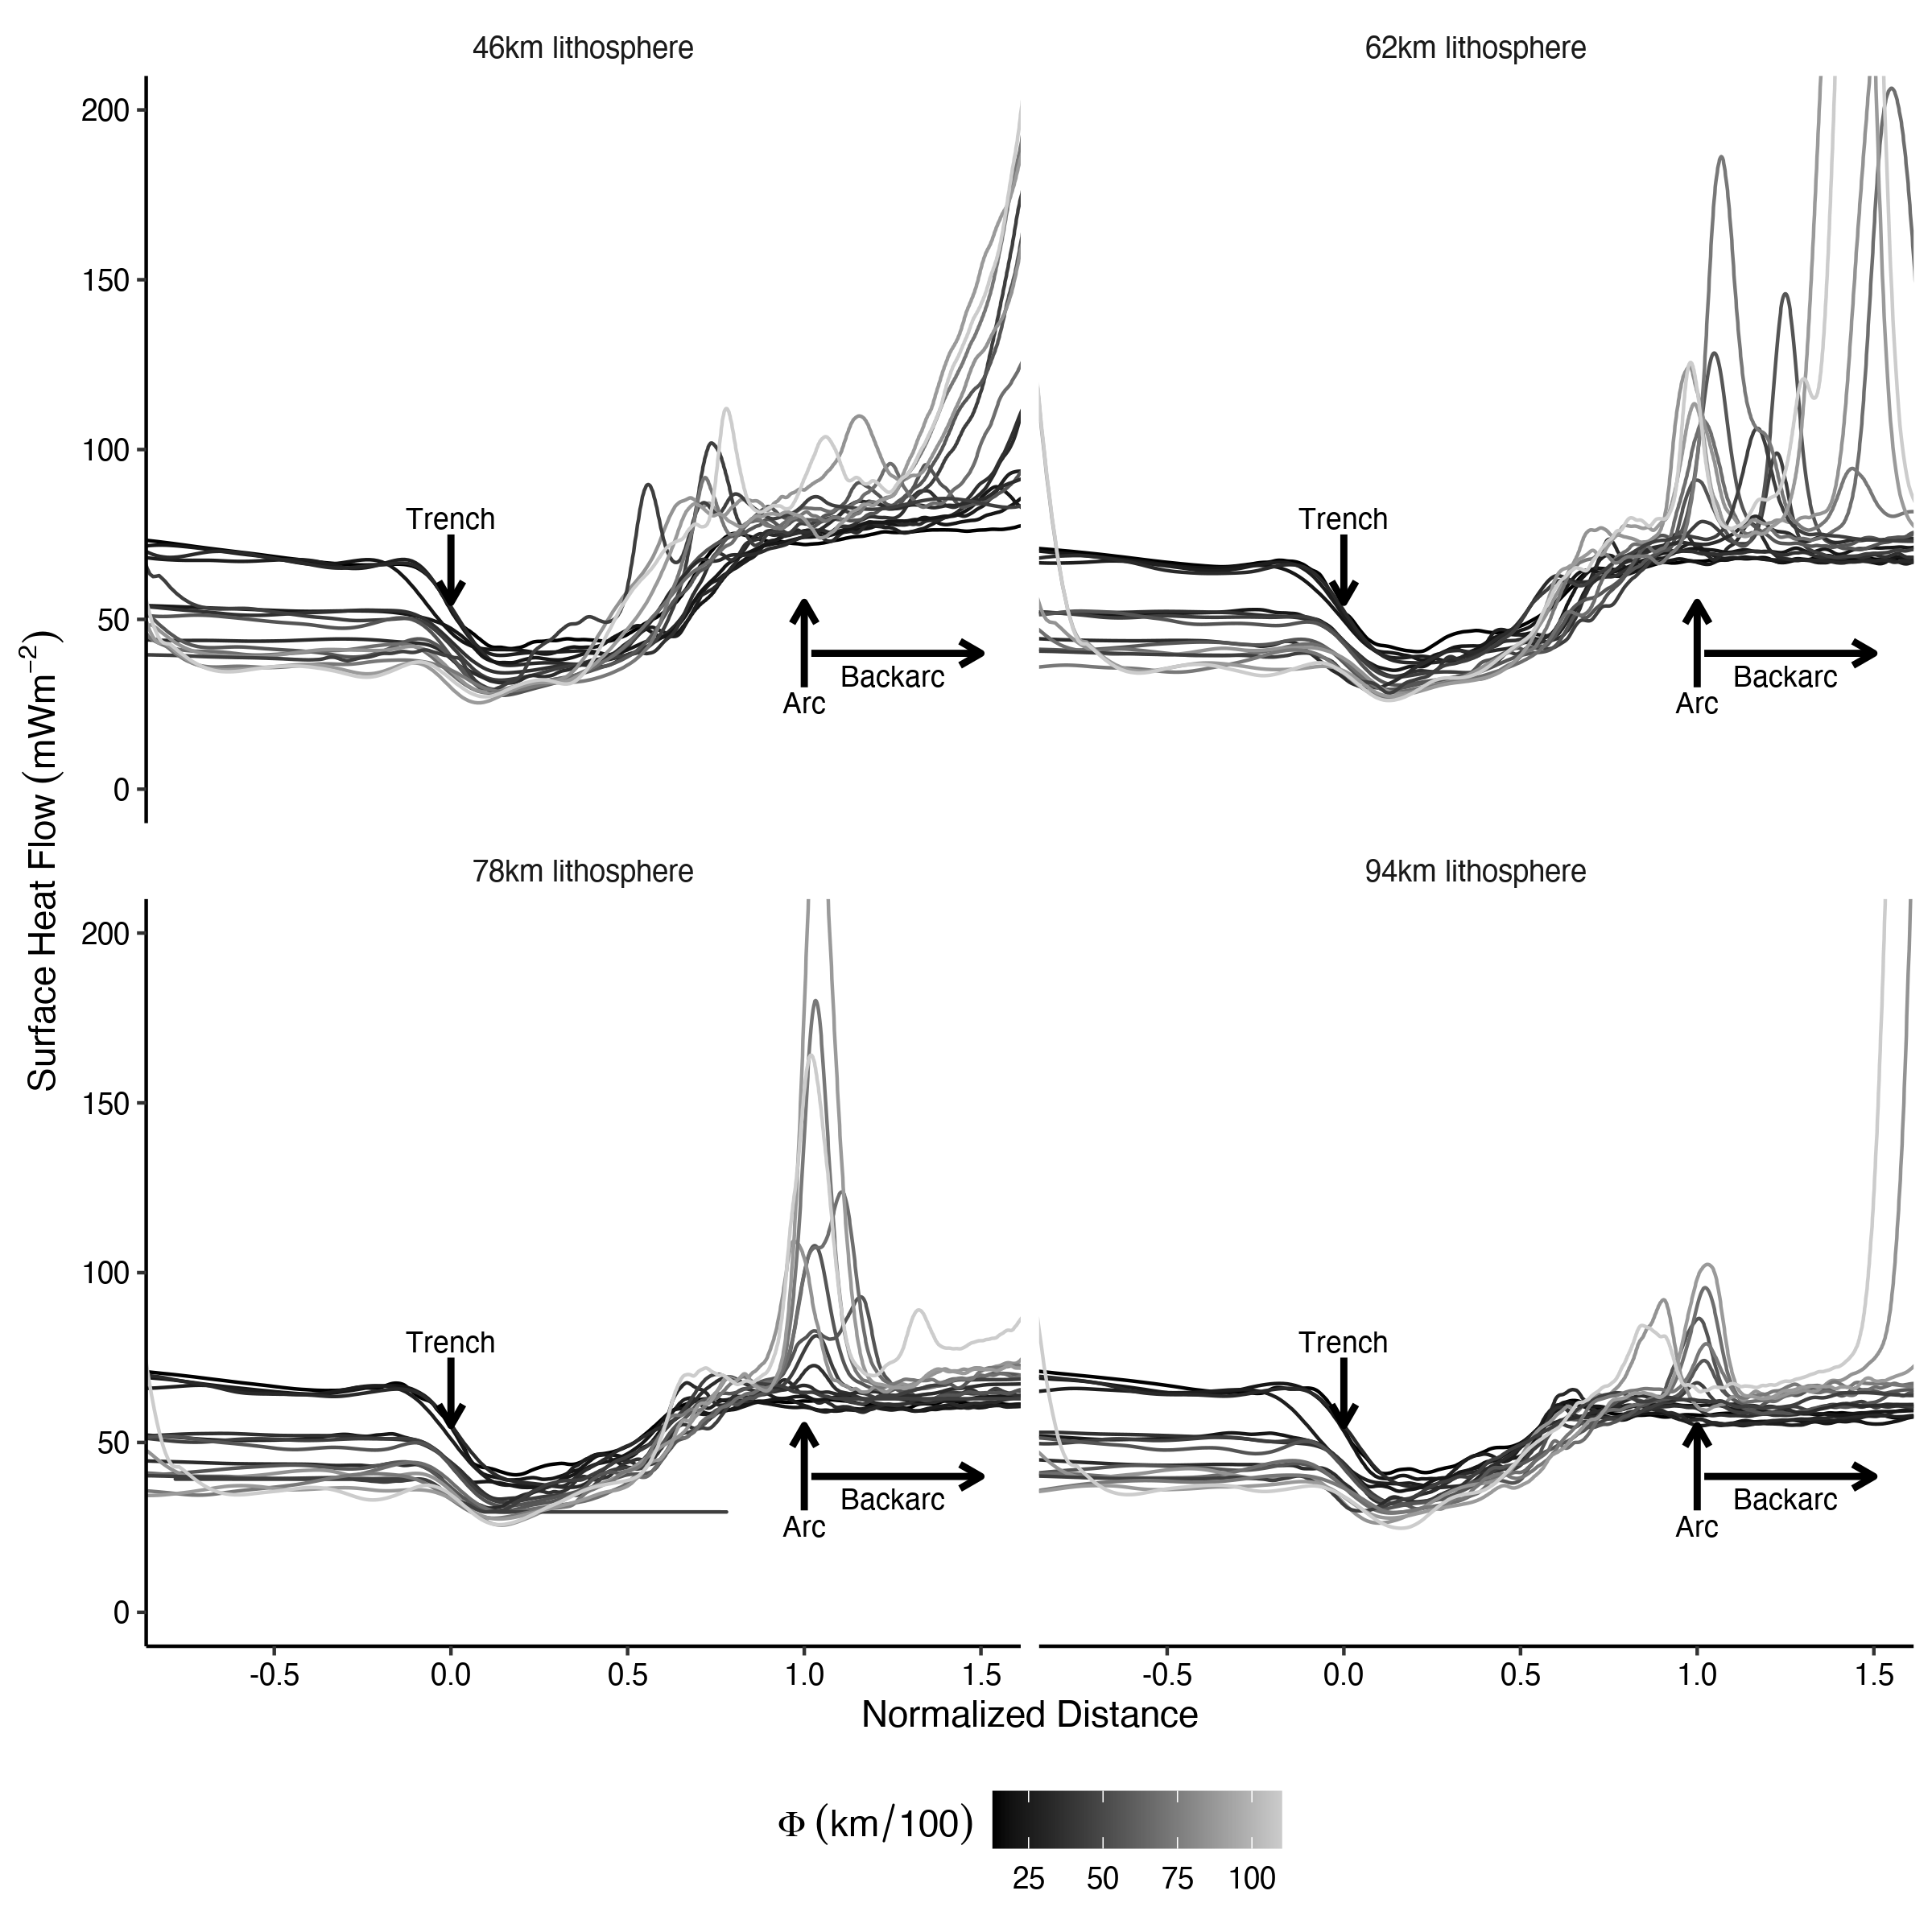
\includegraphics[width=1\linewidth,]{figs/fig7}

}

\caption{Surface heat flow vs. normalized distance for numerical models with backarc lithospheric thicknesses of 46, 62, 78, and 94 $km$. Normalized distance is the true distance relative to the trench divided by the distance between the arc and trench. Heat flow is colored according to the slab thermal parameter. High amplitude fluctuations in heat flow in the arc region (normalized distance = 1.0) correspond to vertical migration of fluids and melts. In the backarc region, these fluctuations correspond to backarc extension associated with the oldest and fastest-moving slabs (lighter gray lines). Models with no extension fall within a narrow range of surface heat flow values in the backarc region (darker gray lines).}\label{fig:hf}
\end{figure}
\DIFaddend

\DIFaddbegin \clearpage

\DIFaddend \section{Discussion}
\DIFaddbegin

\DIFaddend \subsection{Reaction Mechanism and Thermal Controls on Slab-Mantle
Mechanical coupling}
\DIFaddbegin

\DIFaddend In our numerical experiments, slab-mantle mechanical coupling is
spatially associated with the reaction of (weak) antigorite to form
(stronger) wet olivine. An antigorite-rich serpentinized subduction
channel spontaneously forms atop the dehydrating slab, localizing
strain, lubricating the slab-mantle interface, and mechanically
decoupling the slab and mantle wedge \DIFdelbegin %DIFDELCMD < \cite<e.g.,>[]{Ruh2015, Agard2016}%%%
\DIFdel{.}\DIFdelend \DIFaddbegin \DIFadd{(e.g., Agard et al., 2016; Ruh et
al., 2015). }\DIFaddend As anticipated, it is the viscosity increase resulting from
the transformation of antigorite \DIFdelbegin \DIFdel{($\eta \approx 10^17$) to wet olivine ($\eta \approx 10^23$) }\DIFdelend that causes slab-mantle mechanical
coupling in our models, where the depth of this reaction is primarily
controlled by a balance of competing thermal feedbacks acting in the
upper plate. Cooling and hydration of the upper lithospheric mantle
wedge (antigorite stabilization) and heating from the lower circulating
asthenospheric mantle wedge (antigorite destabilization) compete to fix
the antigorite-out reaction at depth (\DIFdelbegin \DIFdel{Fig.~\ref{Figure9}}\DIFdelend \DIFaddbegin \DIFadd{Figure~\ref{fig:arrows}}\DIFaddend ).

\DIFdelbegin %DIFDELCMD < \begin{figure}
%DIFDELCMD <  \centering
%DIFDELCMD <  
\includegraphics[width=\textwidth, trim={0 0 0 0}]{figs/Fig9.png}
%DIFDELCMD <  \caption{Visualization of an effective P\'{e}clet number and viscosity near the coupling region at $\sim$10 $Ma$ for model cdf with lithospheric thickness of 78 $km$. (a) Effective P\'{e}clet number. Advection dominates transport of heat towards the coupling point (thin dark red region in the asthenospheric mantle wedge), whereas diffusion contributes significantly to transport of heat away from the coupling point by the slab (yellow-green region within the slab). (b) Viscosity. Coupling occurs at the point where the viscosity contrast between the slab and mantle approaches zero. The layer of small cyan-green dots of lower viscosity in the slab reflect serpentine alteration that occurred along bending faults near the trench. Reference points a-e are used for discussing reaction mechanisms and thermal feedbacks during the transition to slab-mantle mechanical coupling.}
%DIFDELCMD <  \label{Figure9}
%DIFDELCMD < \end{figure}
%DIFDELCMD < %%%
\DIFdelend \DIFaddbegin \begin{figure}[h]

{\centering 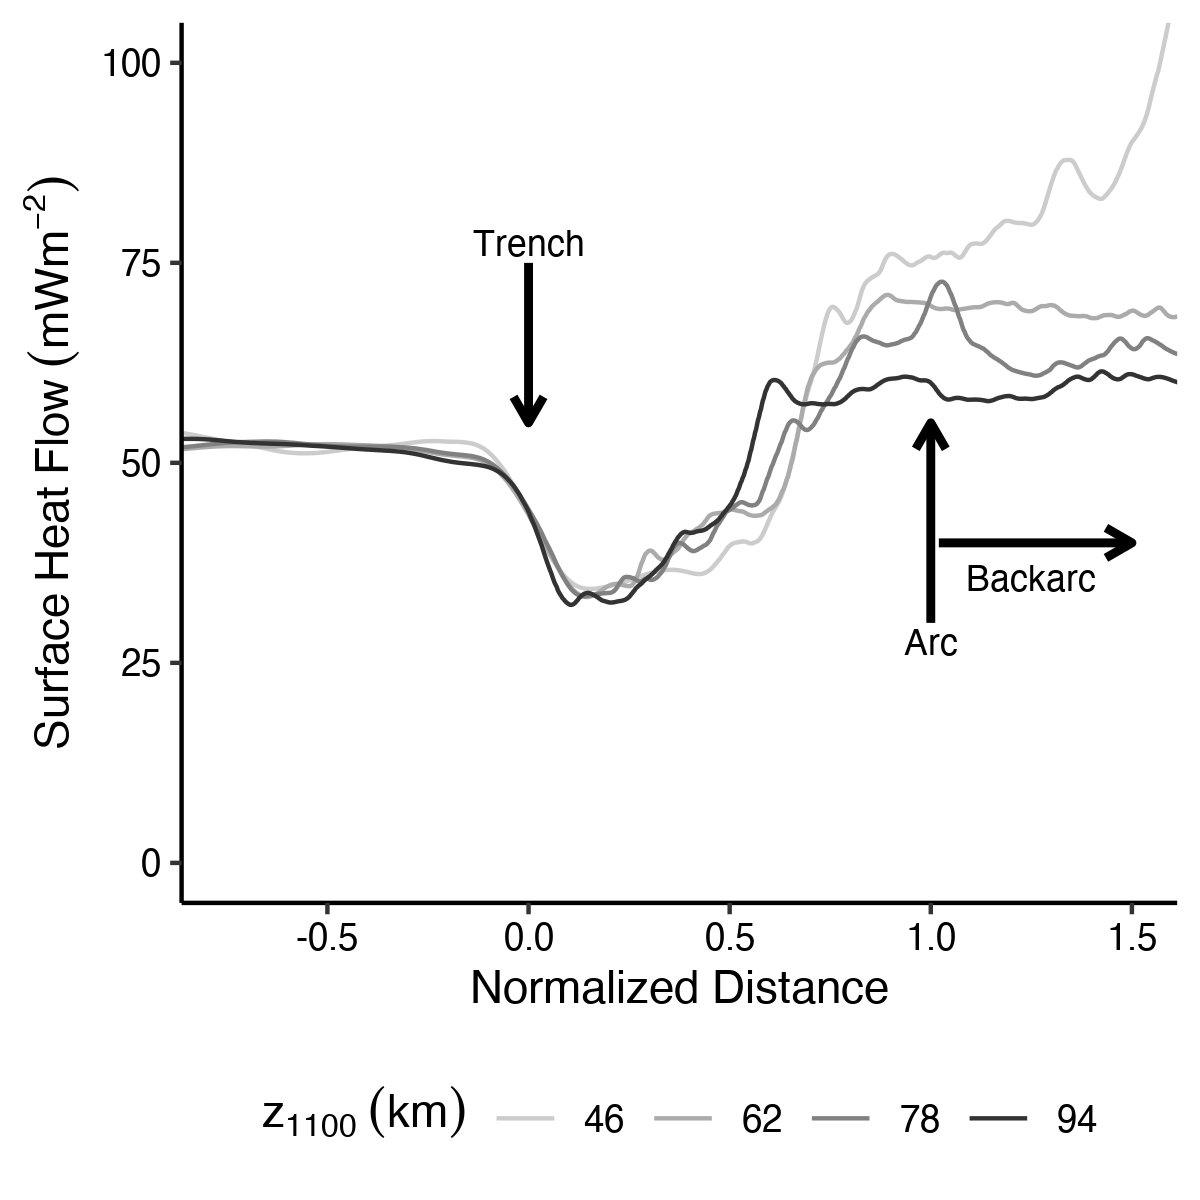
\includegraphics[width=0.8\linewidth,]{figs/fig8}

}

\caption{Surface heat flow vs. normalized distance for model cdf with backarc lithospheric thicknesses ranging from 46 to 94 $km$. The range of surface heat flow values in the forearc (normalized distance between 0.0 and 1.0) is narrow and shows little variance until near the arc (normalized distance between 0.75 and 1.0). Surface heat flow broadly disperses in the backarc (normalized distance $>$ 1.0) and reflects the initial continental geotherm (lithospheric thickness). A simple relationship between surface heat flow and lithospheric thickness may be obscured in any region experiencing an addition of heat from extension or vertical migration of fluids, especially within the arc-region.}\label{fig:hf78}
\end{figure}
\DIFaddend

The entire process can be conceptualized \DIFdelbegin \DIFdel{in terms of an effective P\'{e}clet number}\DIFdelend \DIFaddbegin \DIFadd{as follows}\DIFaddend . Cooling of the
mantle wedge occurs mainly via diffusive heat loss to the slab along the
entire length of the subducted slab-top \DIFdelbegin \DIFdel{, as indicated by the bowed isotherms and relatively low (-20 $<$ Pe $<$ 20) effective P\'{e}clet values along the slab-mantle interface (Fig.~\ref{Figure9}}\DIFdelend \DIFaddbegin \DIFadd{(Figure~\ref{fig:arrows}}\DIFaddend a). At
shallow levels, water released from the slab stabilizes serpentine in
the overriding mantle, effectively decoupling the slab mechanically from
the mantle (\DIFdelbegin \DIFdel{Fig.~\ref{Figure9}}\DIFdelend \DIFaddbegin \DIFadd{Figure~\ref{fig:arrows}}\DIFaddend b, point a). This mechanical
decoupling promotes antigorite stabilization to greater depths because
the mantle wedge stagnates and continues to cool and receive water from
the dehydrating \DIFdelbegin \DIFdel{slab\textemdash a }\DIFdelend \DIFaddbegin \DIFadd{slab---a }\DIFaddend positive feedback for the formation of
serpentinite. \DIFdelbegin \DIFdel{Stagnation is evident by near-zero effective P\'{e}clet values within the lithospheric mantle wedge (Fig.~\ref{Figure9}a ). We note that the warm-colored band that tracks the minimum thermal gradient does not indicate unusually efficient advective heat transport (the numerator of equation~\ref{Equation5} is not especially large), but rather inefficient diffusive heat transport in the context of a small thermal gradient (the denominator of equation~\ref{Equation5} is small)}\DIFdelend \DIFaddbegin \DIFadd{Only a thin layer of serpentine forms at the slab-mantle
interface in our models, but it is sufficient to mechanically decouple
the slab and mantle}\DIFaddend .

At deeper levels, beyond the stability of antigorite, diffusive heat
loss from the mantle to the slab forms a thickening layer of
\DIFdelbegin \DIFdel{new lithosphere }\DIFdelend \DIFaddbegin \DIFadd{high-viscosity mantle }\DIFaddend atop the slab (\DIFdelbegin \DIFdel{Fig.~\ref{Figure9}}\DIFdelend \DIFaddbegin \DIFadd{Figure~\ref{fig:arrows}}\DIFaddend b, point b).
Downward motion of \DIFdelbegin \DIFdel{this new lithosphere (Fig.~\ref{Figure9}}\DIFdelend \DIFaddbegin \DIFadd{the slab, plus accreated high-viscosity mantle,
(Figure~\ref{fig:arrows}}\DIFaddend b, point b) relative to the deepest extent of
the stiff forearc mantle (\DIFdelbegin \DIFdel{Fig.~\ref{Figure9}}\DIFdelend \DIFaddbegin \DIFadd{Figure~\ref{fig:arrows}}\DIFaddend b, point c) creates a
pressure gradient that attracts flow of the weakest
\DIFdelbegin \DIFdel{materials\textemdash serpentinite }\DIFdelend \DIFaddbegin \DIFadd{materials---serpentinite }\DIFaddend from the up-dip direction
(\DIFdelbegin \DIFdel{Fig.~\ref{Figure9}}\DIFdelend \DIFaddbegin \DIFadd{Figure~\ref{fig:arrows}b}\DIFaddend , point d)\DIFdelbegin \DIFdel{\textemdash and }\DIFdelend \DIFaddbegin \DIFadd{---and }\DIFaddend hot mantle from below
(\DIFdelbegin \DIFdel{Fig.~\ref{Figure9}}\DIFdelend \DIFaddbegin \DIFadd{Figure~\ref{fig:arrows}b}\DIFaddend , point e). Flow of hot mantle into the necking
region between points b and c is analogous to passive asthenospheric
upwelling toward a mid-ocean ridge where two strong cooling lithospheric
plates diverge. Highly efficient heat advection from the warm mantle
wedge core (\DIFdelbegin \DIFdel{dark red stream at T $>$ 1100 $^{\circ}C$; Fig.~\ref{Figure9}a) drives reaction of serpentinite to form wet olivine\textemdash a negative feedback to the formation of
serpentinite}\DIFdelend \DIFaddbegin \DIFadd{Figure~\ref{fig:arrows}a) prevents formation of
sperentine---thus limiting and stabilizing the coupling depth}\DIFaddend .

\DIFdelbegin \DIFdel{It is the finely-tuned balance of serpentine stability\textemdash the }\DIFdelend \DIFaddbegin \DIFadd{Thermal and petrologic feedbacks---the }\DIFaddend addition of water into a
diffusively cooling, shallow mantle to produce serpentine vs.\DIFaddbegin \DIFadd{~}\DIFaddend the
advection of heat from the deeper mantle to prevent \DIFdelbegin \DIFdel{it\textemdash that defines the coupling
depth. }\DIFdelend \DIFaddbegin \DIFadd{it---drive coupling
towards steady-state. Our results imply a finely-tuned balance of
serpentine stability can maintain coupling depths in subduction zones
for 10's of Ma.
}\DIFaddend

\subsection{\DIFdelbegin \DIFdel{The impact of $z_{1100}$ and $\Phi$ on coupling}\DIFdelend \DIFaddbegin \texorpdfstring{The impact of \(z_{1100}\) and \(\Phi\) on
coupling}{The impact of z\_\{1100\} and \textbackslash Phi on coupling}\DIFaddend }
\DIFaddbegin

\DIFaddend How does backarc lithospheric thickness (\DIFdelbegin \DIFdel{$z_{1100}$}\DIFdelend \DIFaddbegin \DIFadd{\(z_{1100}\)}\DIFaddend ) influence
coupling depth? The \DIFdelbegin \DIFdel{lithosphere}%DIFDELCMD < \allowbreak%%%
\DIFdel{-asthenosphere }\DIFdelend \DIFaddbegin \DIFadd{lithosphere-asthenosphere }\DIFaddend boundary of the upper
plate defines the permissible flow field of circulating upper mantle,
limiting highly efficient heat advection to below the base of the
mechanical lithosphere (\DIFdelbegin \DIFdel{c.f. Fig.~\ref{Figure10}}\DIFdelend \DIFaddbegin \DIFadd{Figure~\ref{fig:streams}}\DIFaddend a-d). Thin upper plate
lithospheres (\DIFdelbegin \DIFdel{Fig.~\ref{Figure10}}\DIFdelend \DIFaddbegin \DIFadd{Figure~\ref{fig:streams}}\DIFaddend a, b) permit shallower mantle
wedge circulation and advection of heat farther up the subduction
interface. This shallow circulation raises the depth of the serpentine
breakdown reaction and mechanical coupling. Thick upper plate
lithospheres (\DIFdelbegin \DIFdel{Fig.~\ref{Figure10}}\DIFdelend \DIFaddbegin \DIFadd{Figure~\ref{fig:streams}}\DIFaddend c, d) restrict mantle wedge
circulation and advection of heat to deeper levels, shifting the
serpentine breakdown reaction and mechanical coupling to greater depths.

\DIFdelbegin %DIFDELCMD < \begin{figure}
%DIFDELCMD <  \centering
%DIFDELCMD <  \includegraphics[width=\textwidth,  trim={0 0 0 0}]{figs/Fig10.png}
%DIFDELCMD <  \caption{Variation in effective P\'{e}clet number for the standard model, cdf, with backarc lithospheric thickness of (a) 46, (b) 62, (c) 78, and (d) 94 $km$. All models are visualized at $\sim$10 $Ma$ and plotted on the same scale and location within the model domain. All models display broadly similar distributions of an effective P\'{e}clet number, but the thin dark red streams focus on the subduction interface at different depths. In each model, the thin red stream flowing towards the coupling point is limited to the base of the upper-plate lithosphere, $z_{1100}$.}
%DIFDELCMD <  \label{Figure10}
%DIFDELCMD < \end{figure}
%DIFDELCMD <

%DIFDELCMD < %%%
\DIFdelend In our models, the thermal state of the slab, as represented by the
thermal parameter (\DIFdelbegin \DIFdel{$\Phi$}\DIFdelend \DIFaddbegin \DIFadd{\(\Phi\)}\DIFaddend ), has almost no effect on the mechanical
coupling depth. Previous studies of modern subduction zones also
concluded that coupling appears to be insensitive to slab age and
convergence velocity \DIFdelbegin %DIFDELCMD < \cite{Furukawa1993, Wada2009}%%%
\DIFdelend \DIFaddbegin \DIFadd{(Furukawa, 1993; Wada \& Wang, 2009)}\DIFaddend . The likely
reason that \DIFdelbegin \DIFdel{$\Phi$ }\DIFdelend \DIFaddbegin \DIFadd{\(\Phi\) }\DIFaddend makes so little difference is because slab dynamics
\DIFdelbegin \DIFdel{drive mantle wedge circulation and mantle wedge cooling in opposite directions}\DIFdelend \DIFaddbegin \DIFadd{induce a negative feedback between diffusive cooling and advective
heating}\DIFaddend . High-\DIFdelbegin \DIFdel{$\Phi$ }\DIFdelend \DIFaddbegin \DIFadd{\(\Phi\) }\DIFaddend slabs (older slabs with higher velocities) cool
the mantle wedge more effectively, but also result in stronger mantle
circulation and greater heat advection. In contrast, low-\DIFdelbegin \DIFdel{$\Phi$ }\DIFdelend \DIFaddbegin \DIFadd{\(\Phi\) }\DIFaddend slabs
(younger slabs with lower velocities) are less effective in cooling the
mantle wedge, but also result in weaker mantle circulation and less heat
advection. That is, the shallow vs.\DIFaddbegin \DIFadd{~}\DIFaddend deep impacts of \DIFdelbegin \DIFdel{$\Phi$ }\DIFdelend \DIFaddbegin \DIFadd{\(\Phi\) }\DIFaddend tend to
cancel each other, explaining the lack of strong correlation between
coupling and thermal parameter.

\DIFaddbegin \begin{figure}[h]

{\centering 
\includegraphics[width=1\linewidth,]{figs/fig9}

}

\caption{Visualization of temperature, viscosity, and velocity near the coupling region at $\sim$ 10 $Ma$ for model cdf with lithospheric thickness of 78 $km$. Velocity arrows are relative to the model boundaries, so the upper mantle wedge has a leftwards velocity equal to the velocity of the upper plate, but is stagnant with respect to itself. (a) High-velocity mantle flow occurs only beneath the lithospheric base (1100$^{\circ}C$), transfering heat towards the coupling region. (b) Log viscosity indicates coupling at the point where the viscosity contrast between the slab and mantle approaches zero. Reference points a-e are used for discussing reaction mechanisms and thermal feedbacks during the transition to slab-mantle mechanical coupling.}\label{fig:arrows}
\end{figure}

\clearpage

\DIFaddend \subsection{Predicting Coupling Depths in Subduction Zones}
\DIFaddbegin

\DIFaddend Theoretically, coupling depth can be predicted directly from forearc
heat flow using forward modelling techniques to fit surface heat flow
data \DIFdelbegin %DIFDELCMD < \cite<e.g.,>[]{Wada2009}%%%
\DIFdel{.}\DIFdelend \DIFaddbegin \DIFadd{(e.g., Wada \& Wang, 2009). }\DIFaddend However, we caution against using
fore-arc heat flow data because a) forward models adjust the mechanical
coupling depth independently from the backarc thermal structure, which
is inconsistent with the inherent link between mechanical coupling and
backarc thermal structure discussed above (e.g.,
\DIFdelbegin \DIFdel{Figs.~\ref{Figure8}, ~\ref{Figure10}), b) data are typically sparser in the forearc region compared to the backarc region  }%DIFDELCMD < \cite{Currie2006}%%%
\DIFdel{, and c) }\DIFdelend \DIFaddbegin \DIFadd{Figures~\ref{fig:hf78}, \ref{fig:streams}), and b) }\DIFaddend shear heating and
crustal plutonism can contribute to surface heat flow in the forearc
\DIFdelbegin %DIFDELCMD < \cite{Gao2014, ReesJones2018}%%%
\DIFdel{, }\DIFdelend \DIFaddbegin \DIFadd{(Gao \& Wang, 2014; Rees Jones et al., 2018), }\DIFaddend complicating any simple
correspondence with coupling depth.

Instead, we recommend predicting mechanical coupling depth in modern
subduction zones based on \DIFdelbegin \DIFdel{equation~\ref{Equation6} and }\DIFdelend \DIFaddbegin \DIFadd{Equation~\ref{eq:zc}, }\DIFaddend estimates of backarc
lithospheric thickness (as estimated from backarc heat flow)\DIFaddbegin \DIFadd{, }\DIFaddend and slab
thermal parameter. The slab thermal parameter is inventoried for most
subduction zone segments \DIFdelbegin %DIFDELCMD < \cite{Syracuse2006}%%%
\DIFdel{, }\DIFdelend \DIFaddbegin \DIFadd{(Syracuse \& Abers, 2006), }\DIFaddend but a corresponding
dataset of lithospheric thicknesses does not exist. Several geophysical
and petrologic methods might be considered for independent estimates of
lithospheric thickness (e.g., seismic velocities, flexure, heat flow,
mantle xenoliths, etc.), but we prefer to focus on backarc surface heat
flow because of its \DIFdelbegin \DIFdel{direct }\DIFdelend correspondence with thermal structure. In this
approach, backarc lithospheric thickness is estimated using simple
one-dimensional heat transport models assuming values for radiogenic
heat production in the crust \DIFdelbegin %DIFDELCMD < \cite<e.g.,>[]{Rudnick1998}%%%
\DIFdel{.}\DIFdelend \DIFaddbegin \DIFadd{(e.g., Rudnick et al., 1998). }\DIFaddend That is, one
can use compiled backarc heat flow data to invert for backarc
lithospheric thickness, calculate the slab thermal parameter from the
product of slab age and convergence velocity, and apply
\DIFdelbegin \DIFdel{equation~\ref{Equation6} }\DIFdelend \DIFaddbegin \DIFadd{Equation~\ref{eq:zc} }\DIFaddend to estimate mechanical coupling depth. Of course,
care must be taken to avoid backarcs with strong extensional deformation
or conspicuous heating from magmatism because heat flow in these regions
will underestimate backarc lithospheric thickness and consequently
underestimate coupling depth.

\DIFaddbegin \begin{figure}[h]

{\centering \includegraphics[width=1\linewidth,]{figs/fig10}

}

\caption{Streamlines for the standard model, cdf, with backarc lithospheric thickness of (a) 46, (b) 62, (c) 78, and (d) 94 $km$. All models are visualized at $\sim$ 10 $Ma$ and plotted on the same scale and location within the model domain. The flow of warm mantle is restricted to below the 1100$^{\circ}C$ isotherm, which corresponds to the base of the backarc lithosphere. A minimum coupling depth appears to exist as models with extremely thin lithospheres (a) exhibit coupling at $\sim$ 70-80 $km$ depth, but increasing $z_{1100}$ increases coupling depth as mantle flow and advective heat transport are diminished.}\label{fig:streams}
\end{figure}

\clearpage

\DIFaddend \subsection{A Common Coupling Depth Globally?}
\DIFaddbegin

\DIFaddend Mechanical coupling depths in subduction zones are commonly assumed to
fall within a narrow range of 70-80 \DIFdelbegin \DIFdel{$km$ }%DIFDELCMD < \cite{Wada2009, Syracuse2010}%%%
\DIFdel{.}\DIFdelend \DIFaddbegin \DIFadd{\(km\) (Syracuse et al., 2010; Wada
\& Wang, 2009). }\DIFaddend We tested the correlation between backarc lithospheric
thickness and coupling depth using the natural dataset compiled by \DIFdelbegin %DIFDELCMD < \citet{Wada2009} %%%
\DIFdel{(Fig.~\ref{Figure6}b, }\DIFdelend \DIFaddbegin \DIFadd{Wada
\& Wang (2009) (Figure~\ref{fig:multiv}}\DIFaddend d). Much of their dataset is
based on \DIFdelbegin %DIFDELCMD < \citet{Currie2006}%%%
\DIFdelend \DIFaddbegin \DIFadd{Currie \& Hyndman (2006)}\DIFaddend , who infer backarc lithospheric
thicknesses for 10 circum-Pacific subduction zones of 50-60 \DIFdelbegin \DIFdel{$km$ }\DIFdelend \DIFaddbegin \DIFadd{\(km\) }\DIFaddend (as
defined by the 1200 \DIFdelbegin \DIFdel{$^{\circ}C$ }\DIFdelend \DIFaddbegin \DIFadd{\(^{\circ}C\) }\DIFaddend isotherm). Backarc lithospheres are
inferred to be relatively thin from uniformly high heat flow (\DIFdelbegin \DIFdel{$>$ }\DIFdelend \DIFaddbegin \DIFadd{\(>\) }\DIFaddend 70
\DIFdelbegin \DIFdel{$mW/m^2$}\DIFdelend \DIFaddbegin \DIFadd{\(mW/m^{2}\)}\DIFaddend ), thermobarometric constraints on mantle xenoliths, and
P-wave velocities \DIFdelbegin %DIFDELCMD < \cite{Currie2006}%%%
\DIFdelend \DIFaddbegin \DIFadd{(Currie \& Hyndman, 2006)}\DIFaddend . The mean value of 82
\DIFdelbegin \DIFdel{$\pm$ }\DIFdelend \DIFaddbegin \DIFadd{\(\pm\) }\DIFaddend 14 \DIFdelbegin \DIFdel{$km$ }\DIFdelend \DIFaddbegin \DIFadd{\(km\) }\DIFaddend (2\DIFdelbegin \DIFdel{$\sigma$}\DIFdelend \DIFaddbegin \DIFadd{\(\sigma\)}\DIFaddend ) for mechanical coupling depths in our
analysis (\DIFdelbegin \DIFdel{Fig.~\ref{Figure6}}\DIFdelend \DIFaddbegin \DIFadd{Figure~\ref{fig:multiv}}\DIFaddend d) roughly matches the preferred depth
inferred from forearc heat flow data for Cascadia and NE Japan \DIFdelbegin %DIFDELCMD < \cite<75-80 $km$;>[]{Wada2009, Syracuse2010}%%%
\DIFdel{, }\DIFdelend \DIFaddbegin \DIFadd{(75-80
\(km\), Syracuse et al., 2010; Wada \& Wang, 2009) \(km\), }\DIFaddend but our
predicted coupling depths (\DIFdelbegin \DIFdel{Fig.~\ref{Figure6}}\DIFdelend \DIFaddbegin \DIFadd{Figure~\ref{fig:multiv}}\DIFaddend d) are distributed
more broadly. For example, omitting Mexico and Nankai because their
\DIFdelbegin \DIFdel{$\Phi$ }\DIFdelend \DIFaddbegin \DIFadd{\(\Phi\) }\DIFaddend values fall outside our modeling domain, predicted coupling
depths range from \DIFdelbegin \DIFdel{$\sim$}\DIFdelend \DIFaddbegin \DIFadd{almost }\DIFaddend 100 \DIFdelbegin \DIFdel{$km$ }\DIFdelend \DIFaddbegin \DIFadd{\(km\) }\DIFaddend (Kyushu) to \DIFdelbegin \DIFdel{$\sim$}\DIFdelend \DIFaddbegin \DIFadd{\(\sim\) }\DIFaddend 65 \DIFdelbegin \DIFdel{$km$ }\DIFdelend \DIFaddbegin \DIFadd{\(km\)
}\DIFaddend (Sumatra and NE Japan\DIFaddbegin \DIFadd{, Table \ref{tab:segs}}\DIFaddend ).

The petrologic record may also provide insight into the consistency of a
mechanical coupling depth. As it approaches the mechanical coupling
depth, the serpentine channel narrows and focuses return flow. The
demise of the serpentine channel at greater depths may provide a natural
barrier such that rocks within the serpentine channel are more likely to
be exhumed than rocks below the channel. If so, the abundance of
blueschists and eclogites whose maximum burial depths are less than the
pinchout of the serpentine channel, i.e., at the mechanical coupling
depth, should be greater than rocks with greater maximum burial depths.
A cumulative probability distribution of data compiled by
\DIFdelbegin %DIFDELCMD < \citet{Penniston2015} %%%
\DIFdelend \DIFaddbegin \DIFadd{Penniston-Dorland et al. (2015) }\DIFaddend shows a distinct kink at an inferred
depth of \DIFdelbegin \DIFdel{$\sim$}\DIFdelend \DIFaddbegin \DIFadd{\(\sim\) }\DIFaddend 80 \DIFdelbegin \DIFdel{$km$ (Fig.~\ref{FigureS2}}\DIFdelend \DIFaddbegin \DIFadd{\(km\) (Figure~\ref{fig:pd15}}\DIFaddend ). Rocks whose peak
metamorphic pressures correspond with depths \DIFdelbegin \DIFdel{$\leq$ }\DIFdelend \DIFaddbegin \DIFadd{\(\leq\) }\DIFaddend 80 \DIFdelbegin \DIFdel{$km$ }\DIFdelend \DIFaddbegin \DIFadd{\(km\) }\DIFaddend are much
more likely to be exhumed than rocks metamorphosed at depths \DIFdelbegin \DIFdel{$>$ }\DIFdelend \DIFaddbegin \DIFadd{\(>\) }\DIFaddend 80
\DIFdelbegin \DIFdel{$km$}\DIFdelend \DIFaddbegin \DIFadd{\(km\)}\DIFaddend . In fact, nearly all examples of rocks exhumed from greater
depths in the compilation of \DIFdelbegin %DIFDELCMD < \citet{Penniston2015} %%%
\DIFdelend \DIFaddbegin \DIFadd{Penniston-Dorland et al. (2015) }\DIFaddend were
exhumed in the context of collisions. Logically, the metamorphic record
supports a common mechanical coupling depth of \DIFdelbegin \DIFdel{$\leq$~}\DIFdelend \DIFaddbegin \DIFadd{\(\leq\) }\DIFaddend 80 \DIFdelbegin \DIFdel{$km$}\DIFdelend \DIFaddbegin \DIFadd{\(km\)}\DIFaddend .

Relatively high backarc heat flow\DIFdelbegin \DIFdel{(}\DIFdelend \DIFaddbegin \DIFadd{, }\DIFaddend especially in circum-Pacific
subduction zones\DIFdelbegin \DIFdel{) }\DIFdelend \DIFaddbegin \DIFadd{, }\DIFaddend suggests relatively stable and uniformly thin backarc
lithospheres in mature subduction zones globally that may in turn cause
a common depth of slab-mantle coupling. Although we do not yet fully
understand why the overriding plates may have similar thicknesses, we
can assume that this is likely related to some processes of lithospheric
erosion proposed for subarc lithosphere \DIFdelbegin %DIFDELCMD < \cite<e.g.,>[]{Sobolev2005, Arcay2006, England2010}%%%
\DIFdel{.}\DIFdelend \DIFaddbegin {[}\DIFadd{e.g., Arcay et al. (2006);
England2010; Sobolev \& Babeyko (2005)}{]}\DIFadd{. }\DIFaddend The following mechanisms of
lithospheric erosion have been proposed: lithospheric delamination
induced by lower crust eclogitization \DIFdelbegin %DIFDELCMD < \cite<e.g.,>[]{Sobolev2005}%%%
\DIFdel{, }\DIFdelend \DIFaddbegin \DIFadd{(e.g., Sobolev \& Babeyko, 2005),
}\DIFaddend small-scale convection caused by hydration-induced mantle wedge
weakening \DIFdelbegin %DIFDELCMD < \cite<e.g.,>[]{Arcay2006}%%%
\DIFdel{, thermal erosion }%DIFDELCMD < \cite<e.g.,>[]{England2010} %%%
\DIFdelend \DIFaddbegin \DIFadd{(e.g., Arcay et al., 2006), thermal erosion (e.g., England \&
Katz, 2010) }\DIFaddend and mechanical weakening \DIFdelbegin %DIFDELCMD < \cite<e.g.,>[]{Gerya2011} %%%
\DIFdelend \DIFaddbegin \DIFadd{(e.g., Gerya \& Meilick, 2011) }\DIFaddend by
percolating melts and subarc foundering of magmatic cumulates \DIFdelbegin %DIFDELCMD < \cite<e.g.,>[]{Jull2001}%%%
\DIFdel{.}\DIFdelend \DIFaddbegin \DIFadd{(e.g.,
Jull \& Kelemen, 2001). }\DIFaddend Most of these mechanisms are thus strongly
related to mantle wedge hydration, melting, and melt \DIFdelbegin \DIFdel{transportation }\DIFdelend \DIFaddbegin \DIFadd{transport }\DIFaddend toward
volcanic arcs.

\section{Conclusions}
\DIFaddbegin

\DIFaddend Four important results are highlighted in this study:

\begin{enumerate}
\DIFaddbegin \def\labelenumi{\arabic{enumi}.}
\DIFaddend \item
  The antigorite to olivine dehydration reaction stabilizes where
  balance is achieved between competing thermal feedbacks within the
  stagnant mantle wedge lithosphere (diffusive heat loss and inefficient
  heat advection) and circulating mantle wedge asthenosphere (highly
  efficient and focused heat advection). The depth of this reaction, and
  thus mechanical coupling, is primarily dependent on the mechanical
  thickness of the backarc lithosphere.
\DIFdelbegin %DIFDELCMD <

%DIFDELCMD <  %%%
\DIFdelend \item
  A simple expression fitted to the results of our numerical models
  allows the mechanical coupling depth to be calculated for subduction
  zone segments with adequate surface heat flow data in the backarc
  region. Back-arc lithospheric thickness can be inferred from surface
  heat flow using a one-dimensional steady-state conductive cooling
  model. Together with slab thermal parameter , which is tabulated for
  nearly all subduction segments worldwide \DIFdelbegin %DIFDELCMD < \cite{Syracuse2006, Syracuse2010}%%%
\DIFdel{, }\DIFdelend \DIFaddbegin \DIFadd{(Syracuse et al., 2010;
  Syracuse \& Abers, 2006), }\DIFaddend coupling depth can be calculated using
  \DIFdelbegin \DIFdel{equation~\ref{Equation6}.
}%DIFDELCMD <

%DIFDELCMD <  %%%
\DIFdelend \DIFaddbegin \DIFadd{Equation~\ref{eq:zc}.
}\DIFaddend \item
  Consistently high backarc heat flow in circum-Pacific subduction zones
  \DIFdelbegin %DIFDELCMD < \cite{Currie2006, Wada2009} %%%
\DIFdelend \DIFaddbegin \DIFadd{(Currie \& Hyndman, 2006; Wada \& Wang, 2009) }\DIFaddend may indicate a common
  depth of slab-mantle mechanical coupling globally at ca. 80 \DIFdelbegin \DIFdel{$km$}\DIFdelend \DIFaddbegin \DIFadd{\(km\)}\DIFaddend .
  Prior assumptions of slab-mantle mechanical coupling at 70-80 \DIFdelbegin \DIFdel{$km$ }\DIFdelend \DIFaddbegin \DIFadd{\(km\)
  }\DIFaddend in thermal models \DIFdelbegin \DIFdel{is }\DIFdelend \DIFaddbegin \DIFadd{are broadly }\DIFaddend consistent with our results.
\DIFdelbegin \DIFdel{.
}%DIFDELCMD <

%DIFDELCMD <  %%%
\DIFdelend \item
  As others have proposed \DIFdelbegin %DIFDELCMD < \cite{Currie2006, Wada2009} %%%
\DIFdel{subduction zones appear to }\DIFdelend \DIFaddbegin \DIFadd{(Currie \& Hyndman, 2006; Wada \& Wang, 2009)
  subduction zones may }\DIFaddend self-organize into stable configurations globally
  with warm (thin) upper plate lithospheres and slab-mantle mechanical
  coupling at depths of ca. 80 \DIFdelbegin \DIFdel{$km$}\DIFdelend \DIFaddbegin \DIFadd{\(km\)}\DIFaddend . Questions remain, however,
  including: 1) How do warm (thin) backarcs persist over 100's of
  kilometers throughout the lifespan of subduction zones? 2) How abrupt
  is the antigorite-out reaction along the subduction interface?, and 3)
  How can predictive models like \DIFdelbegin \DIFdel{equation~\ref{Equation6} }\DIFdelend \DIFaddbegin \DIFadd{Equation~\ref{eq:zc} }\DIFaddend be improved using
  natural datasets? We propose these questions as topics for future
  research.
\DIFdelbegin %DIFDELCMD <

%DIFDELCMD < %%%
\DIFdelend \end{enumerate}

\DIFaddbegin \clearpage

\DIFaddend \appendix
\section{\DIFaddbegin \DIFadd{Appendix}\DIFaddend }
\DIFdelbegin \subsection*{\DIFdel{Subduction duration to achieve steady state}}
%DIFAUXCMD
\DIFdelend \DIFaddbegin

\subsection{\DIFadd{Subduction duration to achieve steady state}}

\DIFaddend In our models, the stability depth of antigorite along the slab-mantle
interface increases with time as the subducting slab cools and hydrates
the mantle wedge. We observed this process \DIFdelbegin \DIFdel{proceeding }\DIFdelend for the first 5 \DIFdelbegin \DIFdel{$Ma$ }\DIFdelend \DIFaddbegin \DIFadd{\(Ma\) }\DIFaddend of
subduction with the antigorite stability depth remaining constant for
ca. 10 \DIFdelbegin \DIFdel{$Ma$ afterwards (Fig.~\ref{FigureS1}}\DIFdelend \DIFaddbegin \DIFadd{\(Ma\) afterwards (Figure~\ref{fig:antdepth}}\DIFaddend ). The change in the
antigorite stability depth, and therefore the slab-mantle mechanical
coupling depth, through ca. 10 \DIFdelbegin \DIFdel{$Ma$ }\DIFdelend \DIFaddbegin \DIFadd{\(Ma\) }\DIFaddend emerges self-consistently in our
models and can help explain how similar configurations, in terms of the
depth to the slab beneath arcs \DIFdelbegin %DIFDELCMD < \cite{England2004} %%%
\DIFdelend \DIFaddbegin \DIFadd{(England et al., 2004) }\DIFaddend and thin backarc
lithospheres \DIFdelbegin %DIFDELCMD < \cite{Currie2006}%%%
\DIFdel{, }\DIFdelend \DIFaddbegin \DIFadd{(Currie \& Hyndman, 2006), }\DIFaddend occur in subduction zones with
different slab ages, convergence rates, geometries, and subduction
durations. Our modelling results indicate that subduction zones quickly
(\DIFdelbegin \DIFdel{$<$ }\DIFdelend \DIFaddbegin \DIFadd{\(<\) }\DIFaddend 5 \DIFdelbegin \DIFdel{$Ma$}\DIFdelend \DIFaddbegin \DIFadd{\(Ma\)}\DIFaddend ) develop and stabilize quasi-permanent, generalized
configurations with a slab-mantle mechanical coupling depth dependent on
the thickness of the backarc lithosphere.

Exceptions occur in our models with the thinnest backarc lithospheres
(\DIFdelbegin \DIFdel{$z_{1100}$ }\DIFdelend \DIFaddbegin \DIFadd{\(z_{1100}\) }\DIFaddend = 46 \DIFdelbegin \DIFdel{$km$}\DIFdelend \DIFaddbegin \DIFadd{\(km\)}\DIFaddend ), which \DIFdelbegin \DIFdel{exhibited }\DIFdelend \DIFaddbegin \DIFadd{exhibit }\DIFaddend transient behavior after ca. 5
\DIFdelbegin \DIFdel{$Ma$ (Fig.~\ref{FigureS1}a). Our }\DIFdelend \DIFaddbegin \DIFadd{\(Ma\) (Figure~\ref{fig:antdepth}). These }\DIFaddend models rapidly (\DIFdelbegin \DIFdel{$<$ }\DIFdelend \DIFaddbegin \DIFadd{\(<\) }\DIFaddend 5
\DIFdelbegin \DIFdel{$Ma$}\DIFdelend \DIFaddbegin \DIFadd{\(Ma\)}\DIFaddend ) develop spreading centers in the backarc \DIFdelbegin \DIFdel{for these models }\DIFdelend because of their
extremely thin (weak) backarc lithospheres. The proximity of a spreading
center in the backarc region \DIFdelbegin \DIFdel{could divert enough }\DIFdelend \DIFaddbegin \DIFadd{diverts }\DIFaddend heat from the circulating mantle
wedge \DIFdelbegin \DIFdel{to stabilize antigorite to deeper levels in the forearc than in a similar system that does }\DIFdelend \DIFaddbegin \DIFadd{and interferes with the development of a stable antigorite
breakdown location compared to systems that do }\DIFaddend not develop a backarc
spreading center. \DIFdelbegin \DIFdel{This }\DIFdelend \DIFaddbegin \DIFadd{In principle, diversion of heat to the backarc could
lead to cooler subducting slabs (less heat advection) and deeper
coupling. This hypothesis }\DIFaddend may be tested by artificially increasing the
strength of the backarc lithosphere for models with very thin backarc
lithospheres \DIFaddbegin \DIFadd{to prevent high rates of backarc spreading}\DIFaddend .

\DIFdelbegin \subsection*{\DIFdel{Absolute minimum coupling depths?}}
%DIFAUXCMD
\DIFdelend \DIFaddbegin \begin{figure}[h]

{\centering 
\includegraphics[width=1\linewidth,]{figs/figA1}

}

\caption{The depth of antigorite stability at the slab-mantle interface vs. time for models with 46, 62, 78, and 94 $km$-thick backarc lithospheres. Antigorite stabilization deepens for the first ca. 5 $Ma$ of subduction and then remains roughly constant for ca. 10 $Ma$. The exceptions are models with very thin backarc lithospheres, which exhibit transient behavior for at least 15 $Ma$. The final achieved stability depth of antigorite increases with increasing backarc lithospheric thickness.}\label{fig:antdepth}
\end{figure}

\clearpage

\subsection{\DIFadd{Absolute minimum coupling depths?}}

\DIFaddend The form of our preferred quadratic regression model shows shallowing of
coupling depths decelerating with progressively thinner upper plate
lithospheres, reaching a minimum of ca. 60 \DIFdelbegin \DIFdel{$km$}\DIFdelend \DIFaddbegin \DIFadd{\(km\)}\DIFaddend . This implies that the
antigorite-out reaction should eventually stabilize at \DIFdelbegin \DIFdel{$\geq$ }\DIFdelend \DIFaddbegin \DIFadd{\(\geq\) }\DIFaddend 60
\DIFdelbegin \DIFdel{$km$ }\DIFdelend \DIFaddbegin \DIFadd{\(km\) }\DIFaddend depth even during nascent subduction and in warm systems with
thin upper plate lithospheres. From a theoretical point of view, a thin
upper plate lithosphere could allow high heat transport to the shallow
mantle wedge and hinder stabilization of antigorite \DIFdelbegin \DIFdel{all together}\DIFdelend \DIFaddbegin \DIFadd{altogether}\DIFaddend . Olivine
plus pyroxene would be the stable mantle minerals\DIFaddbegin \DIFadd{, }\DIFaddend and strong, shallow
coupling between plates would be expected \DIFdelbegin %DIFDELCMD < \cite{Gerya2008}%%%
\DIFdel{. }\DIFdelend \DIFaddbegin \DIFadd{Gerya et al. (2008). }\DIFaddend However,
our models show that even the warmest subduction systems eventually
stabilize antigorite in the shallow mantle wedge. This is evident by the
increasing depth of mechanical coupling with time for the first 5 \DIFdelbegin \DIFdel{$Ma$ }\DIFdelend \DIFaddbegin \DIFadd{\(Ma\)
}\DIFaddend of subduction (\DIFdelbegin \DIFdel{Fig.~\ref{FigureS1}}\DIFdelend \DIFaddbegin \DIFadd{Figure~\ref{fig:antdepth}}\DIFaddend ).

\DIFdelbegin %DIFDELCMD < \begin{figure}[H]
%DIFDELCMD <  \centering
%DIFDELCMD <  
\includegraphics[width=\textwidth,  trim={0 0 0 0}]{figs/FigS1.png}
%DIFDELCMD <  \caption{The depth of antigorite stability at the slab-mantle interface vs. time for models with 46 (a), 62 (b), 78 (c), and 94 $km$-thick (d) backarc lithospheres. Antigorite stabilization deepens for the first ca. 5 $Ma$ of subduction and then remains roughly constant for ca. 10 $Ma$. The exceptions are models with very thin backarc lithospheres (a), which exhibit transient behavior for at least 15 $Ma$. The final achieved stability depth of antigorite increases with increasing backarc lithospheric thickness.}
%DIFDELCMD <  \label{FigureS1}
%DIFDELCMD < \end{figure}
%DIFDELCMD < %%%
\DIFdelend \DIFaddbegin \begin{figure}[h]

{\centering 
\includegraphics[width=0.8\linewidth,]{figs/figA2}

}

\caption{Cumulative probability versus peak metamorphic pressures for metamorphic rocks exhumed from subduction zones. The break in slope at ca. 2.5 $GPa$ (ca. 80 $km$) suggests that the relative probability that a rock will exhume from pressures less than ca. 2.5 $GPa$ is substantially greater (steeper slope) than for higher pressure rocks (shallower slope). Nearly all rocks exhumed from pressures greater than ca. 2.5 $GPa$ derive from continental crust and were exhumed during collision. Paucity of data below 0.5 $GPa$ reflects sampling bias because these rocks are at best incipiently metamorphosed and not conducive to thermobarometry.}\label{fig:pd15}
\end{figure}
\DIFaddend

\DIFdelbegin \subsection*{\DIFdel{(De-)hydration model}}
%DIFAUXCMD
\DIFdelend \DIFaddbegin \begin{table}

\caption{\label{tab:anova}Summary of ANOVA test}
\centering
\fontsize{8}{10}\selectfont
\begin{threeparttable}
\begin{tabular}[t]{llrrrl}
\toprule
\multicolumn{1}{c}{Term} & \multicolumn{1}{c}{Contrast} & \multicolumn{1}{c}{Estimate} & \multicolumn{1}{c}{Upper Bound} & \multicolumn{1}{c}{Lower Bound} & \multicolumn{1}{c}{p value} \\
 &  & $km$ & $km$ & $km$ & \\
\midrule
\cellcolor{gray!6}{$z_{1100}$} & \cellcolor{gray!6}{62-46} & \cellcolor{gray!6}{8.3} & \cellcolor{gray!6}{2.5} & \cellcolor{gray!6}{14.0} & \cellcolor{gray!6}{1.84e-03}\\
$z_{1100}$ & 78-46 & 18.0 & 12.3 & 23.7 & 1.08e-10\\
\cellcolor{gray!6}{$z_{1100}$} & \cellcolor{gray!6}{94-46} & \cellcolor{gray!6}{33.6} & \cellcolor{gray!6}{27.8} & \cellcolor{gray!6}{39.3} & \cellcolor{gray!6}{1.99e-11}\\
$z_{1100}$ & 78-62 & 9.8 & 4.0 & 15.5 & 1.83e-04\\
\cellcolor{gray!6}{$z_{1100}$} & \cellcolor{gray!6}{94-62} & \cellcolor{gray!6}{25.3} & \cellcolor{gray!6}{19.6} & \cellcolor{gray!6}{31.0} & \cellcolor{gray!6}{1.99e-11}\\
\addlinespace
$z_{1100}$ & 94-78 & 15.6 & 9.8 & 21.3 & 7.31e-09\\
\bottomrule
\end{tabular}
\begin{tablenotes}
\item Pair-wise Tukey's test comparing means between groups. Estimates are differences between means. Null hypothesis is that means are not different
\end{tablenotes}
\end{threeparttable}
\end{table}

\begin{table}

\caption{\label{tab:reg.summary}Summary of regression models}
\centering
\fontsize{8}{10}\selectfont
\begin{threeparttable}
\begin{tabular}[t]{llrrl}
\toprule
Model & Term & Estimate & Std. Error & p value\\
\midrule
\cellcolor{gray!6}{1} & \cellcolor{gray!6}{Intercept} & \cellcolor{gray!6}{89.4} & \cellcolor{gray!6}{3.7} & \cellcolor{gray!6}{2.24e-33}\\
1 & $\phi$ & -0.1 & 0.1 & 1.55e-01\\
\cellcolor{gray!6}{2} & \cellcolor{gray!6}{Intercept} & \cellcolor{gray!6}{36.4} & \cellcolor{gray!6}{3.2} & \cellcolor{gray!6}{7.15e-17}\\
2 & $z_{1100}$ & 0.7 & 0.0 & 3.73e-23\\
\cellcolor{gray!6}{3} & \cellcolor{gray!6}{Intercept} & \cellcolor{gray!6}{58.9} & \cellcolor{gray!6}{1.7} & \cellcolor{gray!6}{1.43e-41}\\
\addlinespace
3 & $z_{1100}^2$ & 0.0 & 0.0 & 2.98e-24\\
\cellcolor{gray!6}{4} & \cellcolor{gray!6}{Intercept} & \cellcolor{gray!6}{69.2} & \cellcolor{gray!6}{14.0} & \cellcolor{gray!6}{6.25e-06}\\
4 & $z_{1100}$ & -0.3 & 0.4 & 4.63e-01\\
\cellcolor{gray!6}{4} & \cellcolor{gray!6}{$z_{1100}^2$} & \cellcolor{gray!6}{0.0} & \cellcolor{gray!6}{0.0} & \cellcolor{gray!6}{1.95e-02}\\
5 & Intercept & 41.1 & 3.3 & 1.14e-18\\
\addlinespace
\cellcolor{gray!6}{5} & \cellcolor{gray!6}{$z_{1100}$} & \cellcolor{gray!6}{0.7} & \cellcolor{gray!6}{0.0} & \cellcolor{gray!6}{1.12e-24}\\
5 & $\phi$ & -0.1 & 0.0 & 1.18e-03\\
\cellcolor{gray!6}{6} & \cellcolor{gray!6}{Intercept} & \cellcolor{gray!6}{63.6} & \cellcolor{gray!6}{2.1} & \cellcolor{gray!6}{8.29e-39}\\
6 & $z_{1100}^2$ & 0.0 & 0.0 & 5.68e-26\\
\cellcolor{gray!6}{6} & \cellcolor{gray!6}{$\phi$} & \cellcolor{gray!6}{-0.1} & \cellcolor{gray!6}{0.0} & \cellcolor{gray!6}{6.98e-04}\\
\addlinespace
7 & Intercept & 73.8 & 12.9 & 3.39e-07\\
\cellcolor{gray!6}{7} & \cellcolor{gray!6}{$z_{1100}$} & \cellcolor{gray!6}{-0.3} & \cellcolor{gray!6}{0.4} & \cellcolor{gray!6}{4.23e-01}\\
7 & $z_{1100}^2$ & 0.0 & 0.0 & 1.12e-02\\
\cellcolor{gray!6}{7} & \cellcolor{gray!6}{$\phi$} & \cellcolor{gray!6}{-0.1} & \cellcolor{gray!6}{0.0} & \cellcolor{gray!6}{7.28e-04}\\
\bottomrule
\end{tabular}
\begin{tablenotes}
\item 1=$z_c$=$\phi$, 2=$z_c$=$z_{1100}$, 3=$z_c$=$z_{1100}^2$, 4=$z_c$=$z_{1100}+z_{1100}^2$, 5=$z_c$=$z_{1100}+\phi$, 6=$z_c$=$z_{1100}^2+\phi$, 7=$z_c$=$z_{1100}+z_{1100}^2+\phi$
\end{tablenotes}
\end{threeparttable}
\end{table}

\clearpage

\subsection{\DIFadd{(De-)hydration model}}

\DIFaddend The material properties used in our experiments are listed in \DIFdelbegin \DIFdel{Table~\ref{Table1} \& Table~\ref{Table2}}\DIFdelend \DIFaddbegin \DIFadd{Tables
\ref{tab:materials} and \ref{tab:melts}}\DIFaddend . For details about the
sedimentation and erosion, melting and extraction, and rheological
models, please refer to \DIFdelbegin %DIFDELCMD < \citet{Sizova2010}%%%
\DIFdel{. Here we only discuss }\DIFdelend \DIFaddbegin \DIFadd{Sizova et al. (2010). Here we discuss only }\DIFaddend the
hydrodynamic model, because it is the most relevant aspect of our
results.

The hydrodynamics in our models \DIFdelbegin \DIFdel{are especially relevant to our results and conclusions since it }\DIFdelend controls the timing and magnitude of
mantle wedge hydration. The main sources of water delivered to the
mantle are altered basaltic crust and seafloor sediments, which we
assumed \DIFaddbegin \DIFadd{to }\DIFaddend contain up to 5 \DIFdelbegin \DIFdel{$wt.\% H_2O$}\DIFdelend \DIFaddbegin \DIFadd{\(wt.\% H_{2}O\)}\DIFaddend . We assumed a gradual
expulsion of water from pore space and through quasi-continuous
dehydration reactions occurring within the slab. Water content is
computed using the following equation:

\DIFdelbegin %DIFDELCMD < \begin{equation}
%DIFDELCMD <  \chi_{H_2O(wt.\%)}=\chi_{H_2O(p_0)}\times \left(1-\frac{\Delta z}{150\cdot 10^3}\right)
%DIFDELCMD <  \label{EquationS1}
%DIFDELCMD < \end{equation}%%%
\DIFdelend \DIFaddbegin \[\begin{aligned}\chi_{H_{2}O(wt.\%)} = \chi_{H_{2}O(p_{0})} \times \left( 1 - \frac{\Delta z}{150 \cdot 10^{3}} \right)\end{aligned}\]\DIFaddend

where \DIFdelbegin \DIFdel{$\chi_{H_2O(p_0)}$}\DIFdelend \DIFaddbegin \DIFadd{\(\chi_{H_{2}O(p_{0})}\)}\DIFaddend =5 \DIFdelbegin \DIFdel{$wt.\%$ and $\Delta z$ }\DIFdelend \DIFaddbegin \DIFadd{\(wt.\%\) and \(\Delta z\) }\DIFaddend is a
marker's depth below the topographical surface.

If a rock marker dehydrates, an independent water particle is
instantaneously generated at the same location with the respective
\DIFdelbegin \DIFdel{$H_2O$ }\DIFdelend \DIFaddbegin \DIFadd{\(H_{2}O\) }\DIFaddend content. The new water particle is moved in accordance to the
local velocity field, described by the following equation:

\DIFdelbegin %DIFDELCMD < \begin{equation}
%DIFDELCMD <  \begin{gathered}
%DIFDELCMD <   v_{water}=(v_x,v_z) \\
%DIFDELCMD <   v_z=v_z-v_{z(percolation)}
%DIFDELCMD <  \end{gathered}
%DIFDELCMD <  \label{EquationS2}
%DIFDELCMD < \end{equation}%%%
\DIFdelend \DIFaddbegin \[\begin{aligned}
v_{\text{water}} & = (v_{x},v_{z}) \\
v_{z} & = v_{z} - v_{z(\text{percolation})} \\
\end{aligned}\]\DIFaddend

where \DIFdelbegin \DIFdel{$v_{water}$ }\DIFdelend \DIFaddbegin \DIFadd{\(v_{water}\) }\DIFaddend is the velocity vector of the water particle,
\DIFdelbegin \DIFdel{$v_x$ and $v_z$ }\DIFdelend \DIFaddbegin \DIFadd{\(v_{x}\) and \(v_{z}\) }\DIFaddend are the local velocity vectors \DIFdelbegin \DIFdel{in the mantle, and $v_{z(percolation)}$ }\DIFdelend \DIFaddbegin \DIFadd{of the the solid
state mantle or crust, and \(v_{z(percolation)}\) }\DIFaddend is a prescribed upward
percolation velocity (10 \DIFdelbegin \DIFdel{$cm/year$}\DIFdelend \DIFaddbegin \DIFadd{\(cm/year\)}\DIFaddend ). We implicitly neglect kinetics of
reactions, as material properties of markers change instantaneously at
equilibrium reactions.

\DIFdelbegin \subsection*{\DIFdel{Approaches for implementing slab-mantle mechanical coupling}}
%DIFAUXCMD
\DIFdelend \DIFaddbegin \subsection{\DIFadd{Approaches for implementing slab-mantle mechanical coupling}}

\DIFaddend Numerical models employ different approaches to simulate the mechanical
decoupling-coupling transition along the slab-mantle interface. A simple
but highly effective approach is to prescribe a weak layer extending
from the surface to some arbitrary depth or temperature that inhibits
transfer of shear stress across the slab-mantle interface. This approach
is analogous to implementing a no-slip condition and effectively
decouples the slab from the mantle. Numerous models use this method
\DIFdelbegin %DIFDELCMD < \cite<e.g.,>[, etc.]{Peacock1996, Peacock1999b, Wada2009, Syracuse2010} %%%
\DIFdelend \DIFaddbegin \DIFadd{(e.g., Peacock, 1996; Peacock \& Wang, 1999; Syracuse et al., 2010; Wada
\& Wang, 2009) }\DIFaddend in part because it allows models to be fine-tuned to
specific subduction zone configurations. Serpentine-or talc-rich
horizons are typically invoked to justify mechanical decoupling along
the shallow interface.

Our approach does not explicitly define slab-mantle mechanical coupling,
rather we use a rheologic model that explicitly follows experimentally
determined flow laws and mineral stability fields. Conceptually, our
approach follows and extends petrologic explanations for a shallow weak
interface\DIFdelbegin \DIFdel{: at }\DIFdelend \DIFaddbegin \DIFadd{. At }\DIFaddend lower temperatures, a hydrated, serpentine-rich\DIFdelbegin \DIFdel{(}\DIFdelend \DIFaddbegin \DIFadd{, }\DIFaddend or
possibly talc-rich\DIFdelbegin \DIFdel{) }\DIFdelend \DIFaddbegin \DIFadd{, }\DIFaddend layer mechanically decouples the mantle wedge from
the subducting slab \DIFdelbegin %DIFDELCMD < \cite{Peacock1999a, Hyndman2003}%%%
\DIFdelend \DIFaddbegin \DIFadd{(Hyndman \& Peacock, 2003; Peacock \& Hyndman,
1999)}\DIFaddend . If so, as a corollary, dehydration of serpentine\DIFdelbegin \DIFdel{(}\DIFdelend \DIFaddbegin \DIFadd{, }\DIFaddend or possibly
talc\DIFdelbegin \DIFdel{) }\DIFdelend \DIFaddbegin \DIFadd{, }\DIFaddend at high temperatures must strengthen the interface. In that
context, and noting that talc is unstable at P \DIFdelbegin \DIFdel{$>$ }\DIFdelend \DIFaddbegin \DIFadd{\(>\) }\DIFaddend 2.0 \DIFdelbegin \DIFdel{$GPa$ }\DIFdelend \DIFaddbegin \DIFadd{\(GPa\) }\DIFaddend in an
ultramafic rock \DIFdelbegin %DIFDELCMD < \cite{Schmidt1998}%%%
\DIFdel{, }\DIFdelend \DIFaddbegin \DIFadd{(Schmidt \& Poli, 1998) \(>\) \(GPa\) , }\DIFaddend we assigned a
serpentine rheology for P-T conditions below the serpentine-out
reaction, and a wet peridotite rheology above it\DIFdelbegin \DIFdel{(where water was present)}\DIFdelend .

To test the sensitivity of coupling on our rheologic model, we ran
diverse experiments that adjusted the rheology of antigorite, the shape
and position of the antigorite-out reaction, and certain hydrodynamic
parameters. For brevity, these results are not presented here. The
experiments included: 1) \DIFdelbegin \DIFdel{Antigorite }\DIFdelend \DIFaddbegin \DIFadd{antigorite }\DIFaddend = wet olivine flow law, 2)
antigorite and wet olivine = dry olivine flow law, 3) isothermal
antigorite \DIFdelbegin \DIFdel{equilibrium }\DIFdelend reaction (straight, vertical reaction line) at 690
\DIFdelbegin \DIFdel{$^{\circ}C$}\DIFdelend \DIFaddbegin \DIFadd{\(^{\circ}C\)}\DIFaddend , 4) \DIFdelbegin \DIFdel{equilibrium }\DIFdelend antigorite reaction with positive nonlinear Clapeyron
slope until 715 \DIFdelbegin \DIFdel{$^{\circ}C$}\DIFdelend \DIFaddbegin \DIFadd{\(^{\circ}C\)}\DIFaddend , where it changes to isothermal (kinked
reaction line), 5) linear \DIFdelbegin \DIFdel{equilibrium }\DIFdelend antigorite reaction with positive Clapeyron
slope (straight, sloped reaction line), 6) linear release of
antigorite-bound \DIFdelbegin \DIFdel{$H_2O$ }\DIFdelend \DIFaddbegin \DIFadd{\(H_{2}O\) }\DIFaddend with depth (instead of abrupt release at
equilibrium dehydration reaction), and 7) no fluid-induced weakening
(pore-pressure = 0).

Only experiments 5 and 7 listed above were inconsistent with the results
presented in the present study. Experiment 5 resulted in transient
coupling depths and disjointed antigorite stability in the mantle wedge,
whereas experiment 7 resulted in two-sided subduction \DIFdelbegin %DIFDELCMD < \cite<e.g.,>[]{Gerya2008}%%%
\DIFdel{.}\DIFdelend \DIFaddbegin \DIFadd{(e.g., Gerya et
al., 2008). }\DIFaddend These experiments suggest that the coupling mechanism in our
models is mostly contingent on the availability of \DIFdelbegin \DIFdel{fluid flux into }\DIFdelend \DIFaddbegin \DIFadd{fluids to }\DIFaddend the mantle
wedge and the shape of the equilibrium antigorite reaction, and
relatively insensitive to the exact flow law parameters.

\DIFdelbegin \subsection*{\DIFdel{Web application for predicting coupling depth}}
%DIFAUXCMD
\DIFdel{Instructions on how to run and use the web-based application and a complete set of tools for reproducing all of the results, tables, and figures presented in this study can be found at }%DIFDELCMD < \url{https://github.com/buchanankerswell/kerswell_et_al_coupling}%%%
\DIFdel{. One can also use the official data repository for this study found at }%DIFDELCMD < \url{https://doi.org/10.17605/OSF.IO/ZJAC3}%%%
\DIFdel{.
}\DIFdelend \DIFaddbegin \begin{figure}[h]

{\centering 
\includegraphics[width=0.8\linewidth,]{figs/figA3}

}

\caption{Visualizations of standard model cdf78 at 1.64 Ma. (a) Rock type. (b) Temperature. (c) Log$_{10}$ of viscosity. (d) Streamlines. Early subduction is facilitated by the prescribed initial weak layer cutting the lithosphere. Strain is localized in the weak serpentine layer at the slab-mantle interface. The mantle wedge is stagnant and loses heat to the slab, which promotes antigorite stabiliization to greater depths. Rock type colors are given in Table \ref{tab:rock.type}.}\label{fig:cdfstep1}
\end{figure}
\DIFaddend

\DIFdelbegin %DIFDELCMD < \begin{threeparttable}[H]
%DIFDELCMD <  \caption{Summary of ANOVA test}
%DIFDELCMD <  \label{TableS1}
%DIFDELCMD <  \setlength{\tabcolsep}{4pt}
%DIFDELCMD <  \begin{tabularx}{\textwidth}{L{1} R{1} R{1} R{1} R{1}}
%DIFDELCMD <

%DIFDELCMD <   \toprule
%DIFDELCMD <

%DIFDELCMD <   Model Comparison & Difference (km) & Lower Bound (km) & Upper Bound (km) & Adj pvalue \\
%DIFDELCMD <

%DIFDELCMD <   \midrule
%DIFDELCMD <

%DIFDELCMD <   62-46 $z_{1100}$ & 8.25            & 2.52             & 14.0             & 2e-03      \\
%DIFDELCMD <   78-46 $z_{1100}$ & 18.0            & 12.3             & 23.7             & 1e-10      \\
%DIFDELCMD <   94-46 $z_{1100}$ & 33.6            & 27.8             & 39.3             & 2e-11      \\
%DIFDELCMD <   78-62 $z_{1100}$ & 9.75            & 4.02             & 15.5             & 2e-04      \\
%DIFDELCMD <   94-62 $z_{1100}$ & 25.3            & 19.6             & 31.0             & 2e-11      \\
%DIFDELCMD <   94-78 $z_{1100}$ & 15.6            & 9.84             & 21.3             & 7e-09      \\
%DIFDELCMD <

%DIFDELCMD <   \bottomrule
%DIFDELCMD <  \end{tabularx}
%DIFDELCMD <  \begin{tablenotes}
%DIFDELCMD <   \footnotesize
%DIFDELCMD <   \item Tukey's post-hoc test for comparing the means of coupling depth between groups
%DIFDELCMD <   of models with different backarc lithospheric thickness. Low pvalues indicate means
%DIFDELCMD <   are actually different
%DIFDELCMD <  \end{tablenotes}
%DIFDELCMD < \end{threeparttable}
%DIFDELCMD < %%%
\DIFdelend \DIFaddbegin \begin{figure}[h]

{\centering 
\includegraphics[width=0.8\linewidth,]{figs/figA4}

}

\caption{Visualization s of standard model cdf78 at 5.05 $Ma$. (a) Rock type. (b) Temperature. (c) Log$_{10}$ of viscosity. (d) Streamlines. By 5 $Ma,$ balance is achieved between heat sinking from the upper mantle wedge to lower parts of the mantle and strong advection of heat in the circulating part of the mantle wedge. A feedback has already developed---heat advection inhibits antigorite stabilization to greater depths. Rock type colors are given in Table \ref{tab:rock.type}.}\label{fig:cdfstep2}
\end{figure}
\DIFaddend

\DIFdelbegin %DIFDELCMD < \begin{threeparttable}[H]
%DIFDELCMD <  \caption{Summary of regression models}
%DIFDELCMD <  \label{TableS2}
%DIFDELCMD <  \begin{tabularx}{\textwidth}{L{1} R{1} R{1} R{1} R{1} R{1} R{1} R{1}}
%DIFDELCMD <

%DIFDELCMD <   \toprule
%DIFDELCMD <

%DIFDELCMD <                               & (1)      & (2)       & (3)         & (4)      & (5)        & (6)         & (7)         \\
%DIFDELCMD <

%DIFDELCMD <   \cmidrule(r){2-8}
%DIFDELCMD <

%DIFDELCMD <   Intercept (km)              & 89.4 *** & 36.4 ***  & 58.9 ***    & 84.8 *** & 41.1 ***   & 63.6 ***    & 89.4 ***    \\
%DIFDELCMD <                               & (3.68)   & (3.19)    & (1.75)      & (0.762)  & (3.26)     & (2.07)      & (1.49)      \\
%DIFDELCMD <   $\frac{\Phi}{100}$ (km/100) & -0.0927  &           &             &          & -0.0927 ** & -0.0927 *** & -0.0927 *** \\
%DIFDELCMD <                               & (0.0644) &           &             &          & (0.0272)   & (0.0260)    & (0.0260)    \\
%DIFDELCMD <   $z_{1100}$ (km)             &          & 0.690 *** &             & 98.8 *** & 0.690 ***  &             & 98.8 ***    \\
%DIFDELCMD <                               &          & (0.0442)  &             & (6.10)   & (0.0409)   &             & (5.59)      \\
%DIFDELCMD <   $z_{1100}^{2}$ (1/km)       &          &           & 0.00495 *** & 14.6 *   &            & 0.00495 *** & 14.6 *      \\
%DIFDELCMD <                               &          &           & (0.000302)  & (6.10)   &            & (0.000277)  & (5.59)      \\
%DIFDELCMD <

%DIFDELCMD <   \cmidrule(r){2-8}
%DIFDELCMD <

%DIFDELCMD <   N                           & 64       & 64        & 64          & 64       & 64         & 64          & 64          \\
%DIFDELCMD <   $R^2$                       & 0.0324   & 0.797     & 0.813       & 0.815    & 0.830      & 0.845       & 0.847       \\
%DIFDELCMD <   p value                     & 2e-01    & 4e-23     & 3e-24       & 5e-23    & 4e-24      & 2e-25       & 2e-24       \\
%DIFDELCMD <

%DIFDELCMD <   \bottomrule
%DIFDELCMD <  \end{tabularx}
%DIFDELCMD <  \begin{tablenotes}
%DIFDELCMD <   \footnotesize
%DIFDELCMD <   \item Models are:
%DIFDELCMD <   (1) = $z_{c}\sim\frac{\Phi}{100}+c$,
%DIFDELCMD <   (2) = $z_{c}\sim{}z_{1100}+c$,
%DIFDELCMD <   (3) = $z_{c}\sim{}z_{1100}^2+c$,
%DIFDELCMD <   (4) = $z_{c}\sim{}z_{1100}+z_{1100}^2+c$,
%DIFDELCMD <   (5) = $z_{c}\sim{}z_{1100}+\frac{\Phi}{100}+c$,
%DIFDELCMD <   (6) = $z_{c}\sim{}z_{1100}^2+\frac{\Phi}{100}+c$,
%DIFDELCMD <   (7) = $z_{c}\sim{}z_{1100}+z_{1100}^2+\frac{\Phi}{100}+c$
%DIFDELCMD <   \item *** p $<$ 0.001;  ** p $<$ 0.01;  * p $<$ 0.05
%DIFDELCMD <   \item Standard Errors in parentheses  (1s.e.)
%DIFDELCMD <  \end{tablenotes}
%DIFDELCMD < \end{threeparttable}
%DIFDELCMD < %%%
\DIFdelend \DIFaddbegin \begin{figure}[h]

{\centering 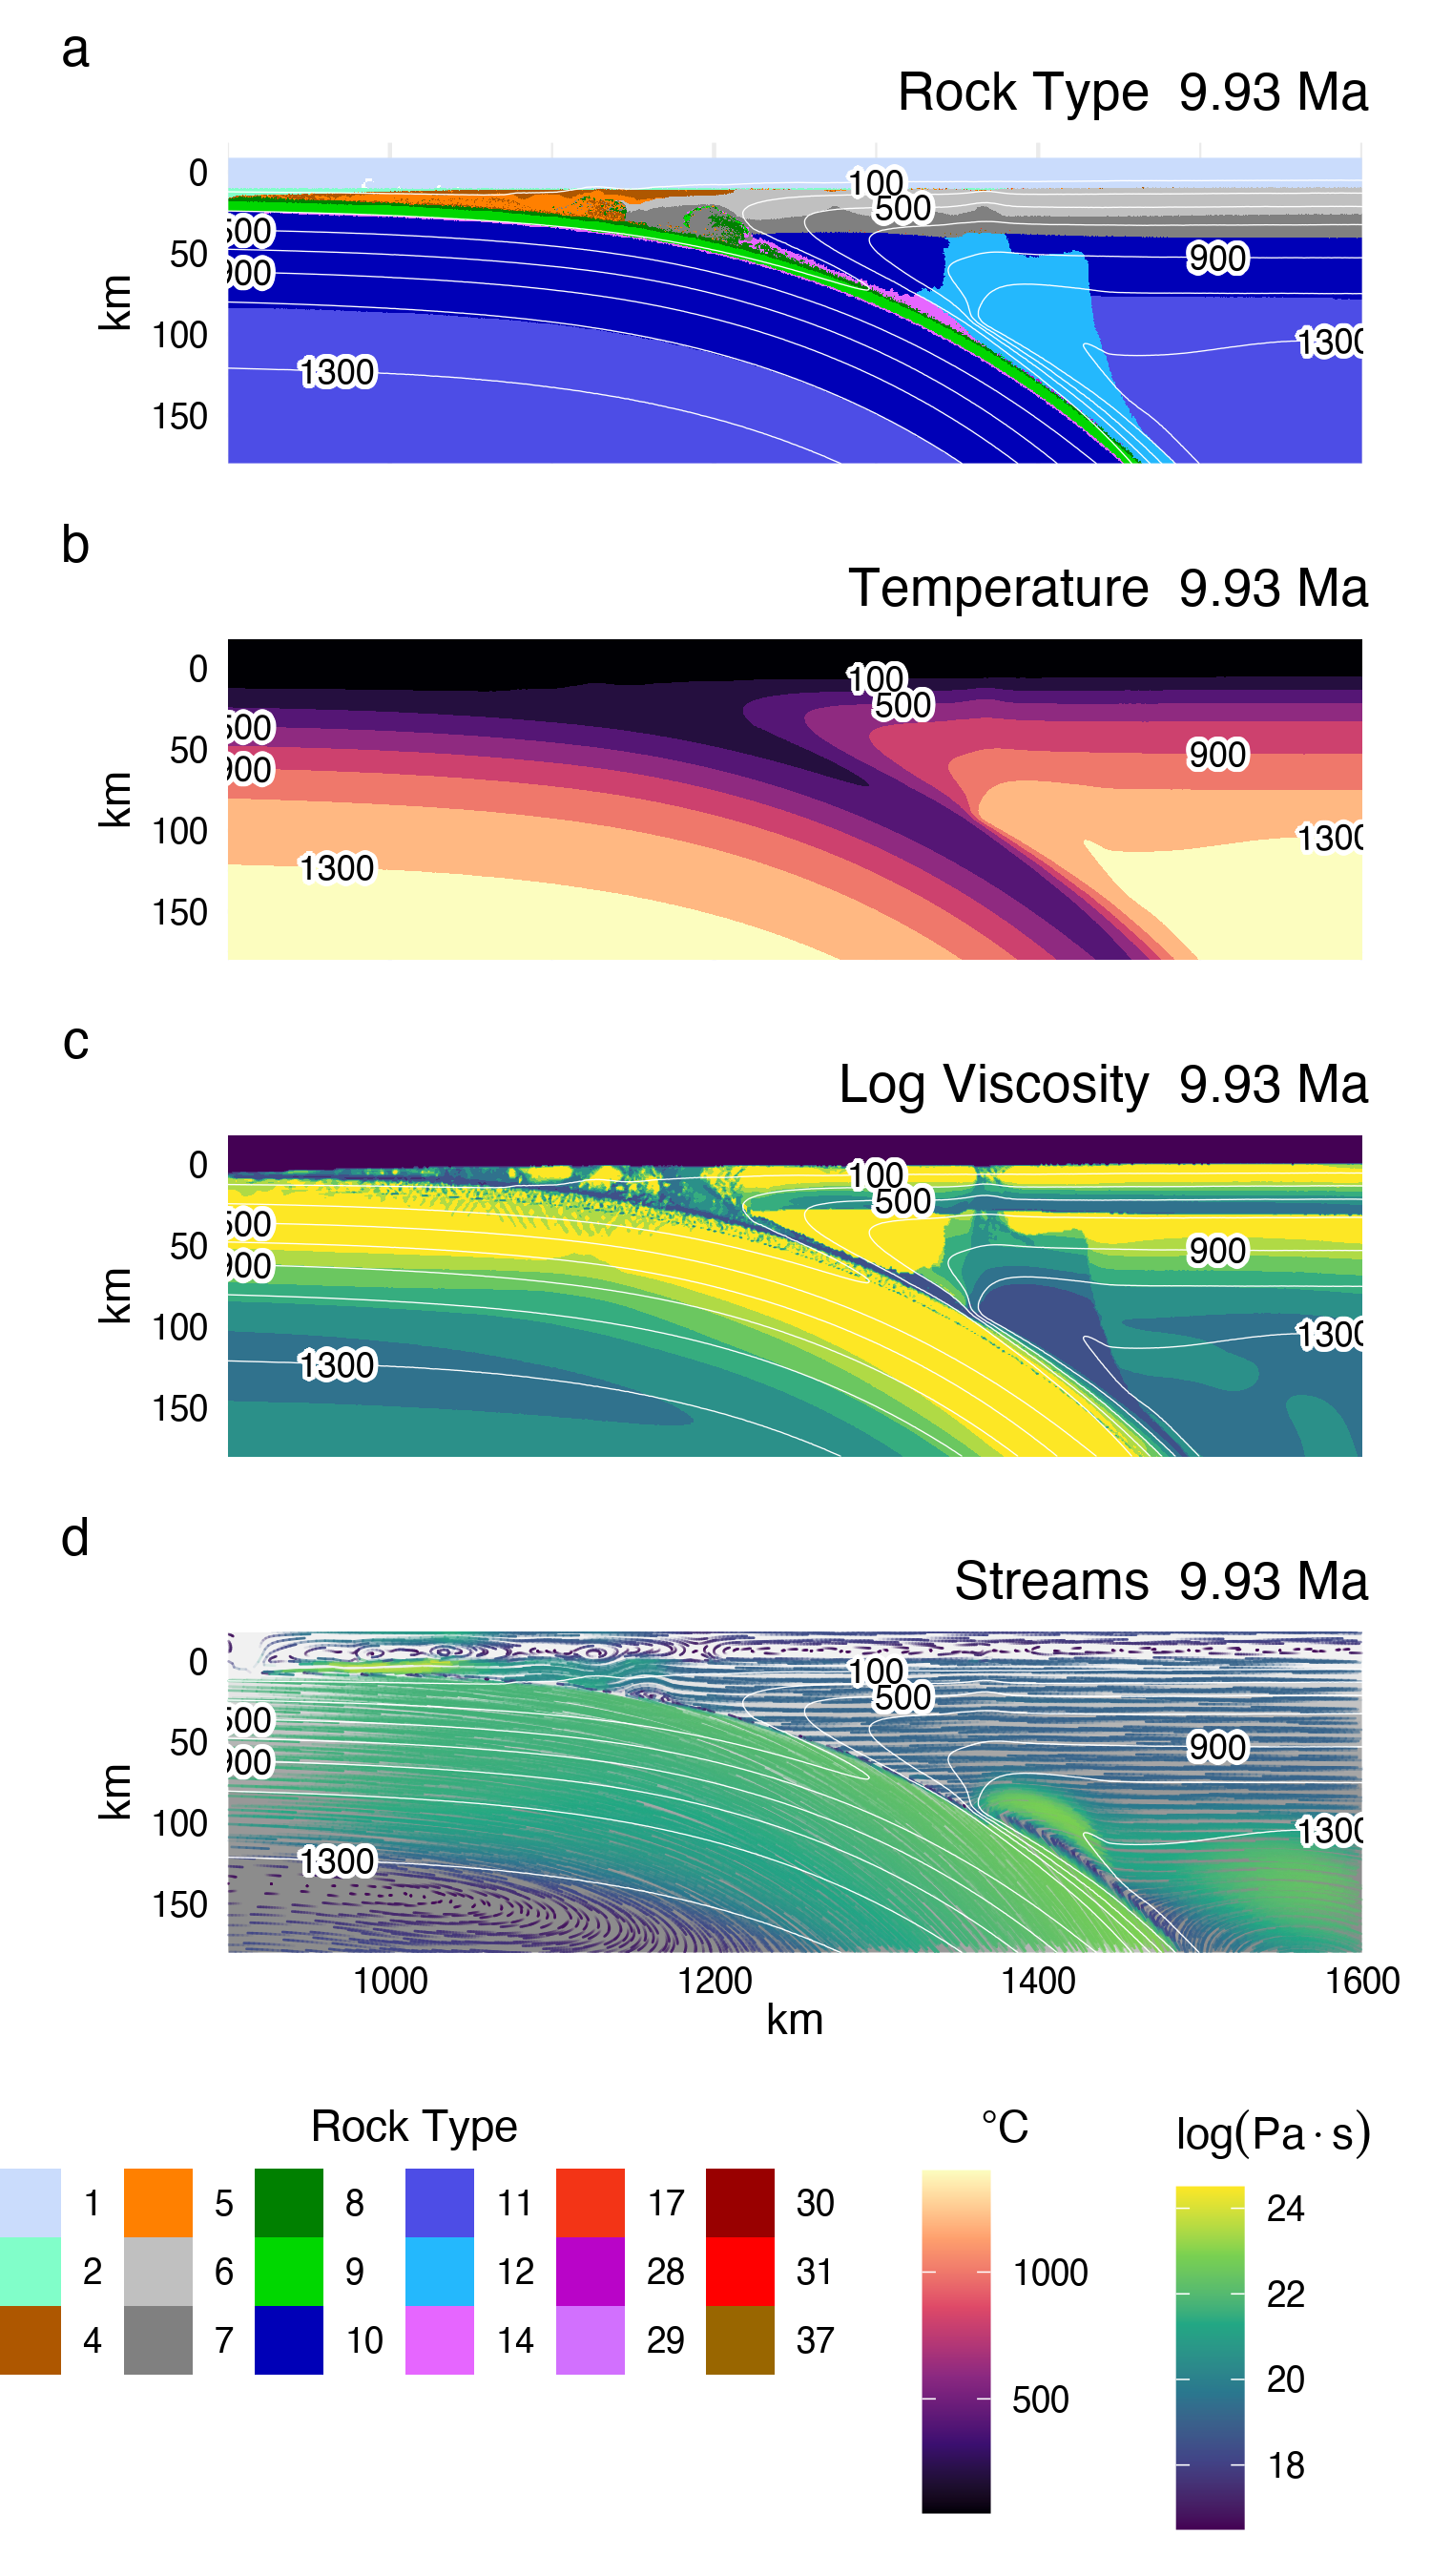
\includegraphics[width=0.8\linewidth,]{figs/figA5}

}

\caption{Visualization s of standard model cdf78 at 9.93 $Ma$. (a) Rock type. (b) Temperature. (c) Log$_{10}$ of viscosity. (d) Streamlines. The geodynamics and thermal structure remain approximately constant from 5 $Ma$ (cf. Figure A.4). The system remains in steady state for as long as enough water is supplied to the upper mantle wedge to stabilize antigorite.Rock type colors are given in Table \ref{tab:rock.type}.}\label{fig:cdfstep3}
\end{figure}
\DIFaddend

\DIFdelbegin %DIFDELCMD < \begin{figure}[H]
%DIFDELCMD <  \centering
%DIFDELCMD <  
\includegraphics[width=0.5\textwidth,  trim={0 0 0 0}]{figs/FigS2.png}
%DIFDELCMD <  \caption{Cumulative probability versus peak metamorphic pressures for metamorphic rocks exhumed from subduction zones. The break in slope at ca. 2.5 $GPa$ (ca. 80 $km$) suggests that the relative probability that a rock will exhume from pressures less than ca. 2.5 $GPa$ is substantially greater (steeper slope) than for higher pressure rocks (shallower slope). Nearly all rocks exhumed from pressures greater than ca. 2.5 $GPa$ derive from continental crust and were exhumed during collision. Paucity of data below 0.5 $GPa$ reflects sampling bias because these rocks are at best incipiently metamorphosed and not conducive to thermobarometry. Data are from \protect\cite{Penniston2015}.}
%DIFDELCMD <  \label{FigureS2}
%DIFDELCMD < \end{figure}
%DIFDELCMD < %%%
\DIFdelend \DIFaddbegin \clearpage
\DIFaddend

\DIFdelbegin %DIFDELCMD < \begin{figure}[H]
%DIFDELCMD <  \centering
%DIFDELCMD <  \includegraphics[width=\textwidth,  trim={0 0 0 0}]{figs/FigS3.png}
%DIFDELCMD <  \caption{Visualization of rock type (a), log viscosity (b), log shear heating (c), effective P\'{e}clet number (d), log stress (e), density (f), and log strain rate (g) for the standard model cdf78 at 1.64 $Ma$. Early subduction is facilitated by the prescribed initial weak layer (high pore fluid pressure) cutting the lithosphere. The P\'{e}clet number in the mantle wedge is less than the P\'{e}clet number of the slab. Heat sinks from the upper mantle wedge to lower in the mantle through thermal diffusion into the slab and advection of that heat downwards by the slab. Antigorite stabilizes to deeper depths.}
%DIFDELCMD <  \label{FigureS3}
%DIFDELCMD < \end{figure}
%DIFDELCMD <

%DIFDELCMD < \begin{figure}[H]
%DIFDELCMD <  \centering
%DIFDELCMD <  \includegraphics[width=\textwidth,  trim={0 0 0 0}]{figs/FigS4.png}
%DIFDELCMD <  \caption{Visualization of rock type (a), log viscosity (b), log shear heating (c), effective P\'{e}clet number (d), log stress (e), density (f), and log strain rate (g) for the standard model cdf78 at 5.05 $Ma$. By 5 $Ma$ balanced is achieved between heat sinking from the upper mantle wedge to lower parts of the mantle by strong advection of heat in the circulating part of the mantle wedge. The ratio of mantle-slab P\'{e}clet number increases abruptly at approx. 80-90 $km$ depth from the surface. A feedback has already developed\textemdash heat advection destabilizing antigorite, resulting in slab-mantle coupling, driving mantle wedge circulation, advecting heat towards the coupling region quicker than can be sunk by the slab.}
%DIFDELCMD <  \label{FigureS4}
%DIFDELCMD < \end{figure}
%DIFDELCMD <

%DIFDELCMD < \begin{figure}[H]
%DIFDELCMD <  \centering
%DIFDELCMD <  \includegraphics[width=\textwidth,  trim={0 0 0 0}]{figs/FigS5.png}
%DIFDELCMD <  \caption{Visualization of rock type (a), log viscosity (b), log shear heating (c), effective P\'{e}clet number (d), log stress (e), density (f), and log strain rate (g) for the standard model cdf78 at 9.93 $Ma$. The geodynamics and thermal structure remain approximately constant from 5 $Ma$ (cf. Fig~\ref{FigureS4}). The system remains in steady state for as long as enough water is supplied to the upper mantle wedge to stabilize antigorite.}
%DIFDELCMD <  \label{FigureS5}
%DIFDELCMD < \end{figure}
%DIFDELCMD <

%DIFDELCMD < \newpage
%DIFDELCMD <

%DIFDELCMD < %%%
\DIFdelend \acknowledgments
\DIFaddbegin

\DIFaddend We thank the Geophysical Fluid Dynamics group at the Institut für
Geophysik, ETH Zürich, for their computing resources and invaluable
instruction, discussion, and support on the numerical modelling methods.
We also thank P. Agard, L. Le Pourhiet, and their students at ISTeP,
Sorbonne Université, for suggestions on the numerical modelling methods
and discussions that greatly enhanced this study. We thank \DIFdelbegin \DIFdel{two }\DIFdelend \DIFaddbegin \DIFadd{the }\DIFaddend anonymous
reviewers for their helpful comments and suggestions, which \DIFdelbegin \DIFdel{prompted our formulation of an effective P\'{e}clet number and }\DIFdelend \DIFaddbegin \DIFadd{greatly
}\DIFaddend improved the manuscript. This work was supported by the National Science
Foundation grant OIA1545903 to M. Kohn, S. Penniston-Dorland, and M.
Feineman. Datasets and tools for reproducing the research in this study
are available at \DIFdelbegin \DIFdel{the official data repository (}%DIFDELCMD < \url{https://doi.org/10.17605/OSF.IO/ZJAC3} %%%
\DIFdel{)or at }%DIFDELCMD < \url{https://github.com/buchanankerswell/kerswell_et_al_coupling}%%%
\DIFdel{. }\DIFdelend \DIFaddbegin \DIFadd{(}\texttt{\DIFadd{https://doi.org/10.17605/OSF.IO/ZJAC3}}\DIFadd{)
}\DIFaddend

\DIFdelbegin %DIFDELCMD < \bibliography{assets/ref}
%DIFDELCMD < %%%
\DIFdelend \DIFaddbegin \newpage

\section*{\DIFadd{References}}
\addcontentsline{toc}{section}{\DIFadd{References}}

\hypertarget{refs}{}
\begin{CSLReferences}{1}{0}
\leavevmode\hypertarget{ref-Abers2017}{}%DIF >
\DIFadd{Abers, G. A., van Keken, P. E., \& Hacker, B. R. (2017). }{\DIFadd{The cold and
relatively dry nature of mantle forearcs in subduction zones}}\DIFadd{.
}\emph{\DIFadd{Nature Geoscience}}\DIFadd{, }\emph{10}(5)\DIFadd{, 333--337.
}

\leavevmode\hypertarget{ref-Agard2009}{}%DIF >
\DIFadd{Agard, P., Yamato, P., Jolivet, L., \& Burov, E. (2009). }{\DIFadd{Exhumation of
oceanic blueschists and eclogites in subduction zones: Timing and
mechanisms}}\DIFadd{. }\emph{\DIFadd{Earth-Science Reviews}}\DIFadd{, }\emph{92}(1-2)\DIFadd{, 53--79.
}

\leavevmode\hypertarget{ref-Agard2016}{}%DIF >
\DIFadd{Agard, P., Yamato, P., Soret, M., Prigent, C., Guillot, S., Plunder, A.,
et al. (2016). }{\DIFadd{Plate interface rheological switches during subduction
infancy: Control on slab penetration and metamorphic sole formation}}\DIFadd{.
}\emph{\DIFadd{Earth and Planetary Science Letters}}\DIFadd{, }\emph{\DIFadd{451}}\DIFadd{, 208--220.
}

\leavevmode\hypertarget{ref-Agrusta2013}{}%DIF >
\DIFadd{Agrusta, R., Arcay, D., Tommasi, A., Davaille, A., Ribe, N., \& Gerya,
T. (2013). }{\DIFadd{Small-scale convection in a plume-fed low-viscosity layer
beneath a moving plate}}\DIFadd{. }\emph{\DIFadd{Geophysical Journal International}}\DIFadd{,
}\emph{194}(2)\DIFadd{, 591--610.
}

\leavevmode\hypertarget{ref-Arcay2006}{}%DIF >
\DIFadd{Arcay, D., Doin, M. P., Tric, E., Bousquet, R., \& Capitani, C. de.
(2006). Overriding plate thinning in subduction zones: Localized
convection induced by slab dehydration. }\emph{\DIFadd{Geochemistry, Geophysics,
Geosystems}}\DIFadd{, }\emph{7}(2)\DIFadd{.
}

\leavevmode\hypertarget{ref-Burg2005}{}%DIF >
\DIFadd{Burg, J. P., \& Gerya, T. (2005). The role of viscous heating in
barrovian metamorphism of collisional orogens: Thermomechanical models
and application to the lepontine dome in the central alps. }\emph{\DIFadd{Journal
of Metamorphic Geology}}\DIFadd{, }\emph{23}(2)\DIFadd{, 75--95.
}

\leavevmode\hypertarget{ref-Carlson2003}{}%DIF >
\DIFadd{Carlson, R. L., \& Miller, D. J. (2003). Mantle wedge water contents
estimated from seismic velocities in partially serpentinized
peridotites. }\emph{\DIFadd{Geophysical Research Letters}}\DIFadd{, }\emph{30}(5)\DIFadd{.
}

\leavevmode\hypertarget{ref-Connolly2005}{}%DIF >
\DIFadd{Connolly, J. A. D. (2005). }{\DIFadd{Computation of phase equilibria by linear
programming: A tool for geodynamic modeling and its application to
subduction zone decarbonation}}\DIFadd{. }\emph{\DIFadd{Earth and Planetary Science
Letters}}\DIFadd{, }\emph{236}(1-2)\DIFadd{, 524--541.
}

\leavevmode\hypertarget{ref-Currie2006}{}%DIF >
\DIFadd{Currie, C. A., \& Hyndman, R. D. (2006). }{\DIFadd{The thermal structure of
subduction zone back arcs}}\DIFadd{. }\emph{\DIFadd{Journal of Geophysical Research}}\DIFadd{,
}\emph{\DIFadd{111}}\DIFadd{(August), 1--22.
}

\leavevmode\hypertarget{ref-Currie2004}{}%DIF >
\DIFadd{Currie, C. A., Wang, K., Hyndman, R. D., \& He, J. (2004). }{\DIFadd{The thermal
effects of steady-state slab-driven mantle flow above a subducting
plate: The Cascadia subduction zone and backarc}}\DIFadd{. }\emph{\DIFadd{Earth and
Planetary Science Letters}}\DIFadd{, }\emph{223}(1-2)\DIFadd{, 35--48.
}

\leavevmode\hypertarget{ref-Cizkova2013}{}%DIF >
\DIFadd{Čížková, H., \& Bina, C. R. (2013). }{\DIFadd{Effects of mantle and
subduction-interface rheologies on slab stagnation and trench rollback}}\DIFadd{.
}\emph{\DIFadd{Earth and Planetary Science Letters}}\DIFadd{, }\emph{\DIFadd{379}}\DIFadd{, 95--103.
}

\leavevmode\hypertarget{ref-Davies1999}{}%DIF >
\DIFadd{Davies, J. H. (1999). }{\DIFadd{The role of hydraulic fractures and intermediate
depth earthquakes in generating suduction zone magmatism}}\DIFadd{.
}\emph{\DIFadd{Nature}}\DIFadd{, }\emph{\DIFadd{417}}\DIFadd{(March), 142--145.
}

\leavevmode\hypertarget{ref-England2010}{}%DIF >
\DIFadd{England, P., \& Katz, R. F. (2010). Melting above the anhydrous solidus
controls the location of volcanic arcs. }\emph{\DIFadd{Nature}}\DIFadd{, }\emph{467}(7316)\DIFadd{,
700--703.
}

\leavevmode\hypertarget{ref-England2004}{}%DIF >
\DIFadd{England, P., Engdahl, R., \& Thatcher, W. (2004). }{\DIFadd{Systematic variation
in the depths of slabs beneath arc volcanoes}}\DIFadd{. }\emph{\DIFadd{Geophysical Journal
International}}\DIFadd{, }\emph{156}(2)\DIFadd{, 377--408.
}

\leavevmode\hypertarget{ref-Faccenda2009}{}%DIF >
\DIFadd{Faccenda, M., Gerya, T., \& Burlini, L. (2009). }{\DIFadd{Deep slab hydration
induced by bending-related variations in tectonic pressure}}\DIFadd{.
}\emph{\DIFadd{Nature Geoscience}}\DIFadd{, }\emph{2}(11)\DIFadd{, 790--793.
}

\leavevmode\hypertarget{ref-Furukawa1993}{}%DIF >
\DIFadd{Furukawa, Y. (1993). }{\DIFadd{Magmatic Processes Under Arcs and Formation of the
Volcanic Front}}\DIFadd{. }\emph{\DIFadd{Journal of Geophysical Research}}\DIFadd{, }\emph{\DIFadd{98}}\DIFadd{,
8309--8319.
}

\leavevmode\hypertarget{ref-Gao2014}{}%DIF >
\DIFadd{Gao, X., \& Wang, K. (2014). }{\DIFadd{Strength of stick-slip and creeping
subduction megathrusts from heat flow observations}}\DIFadd{. }\emph{\DIFadd{Science}}\DIFadd{,
}\emph{345}(6200)\DIFadd{, 1038--1041.
}

\leavevmode\hypertarget{ref-Gao2017}{}%DIF >
\DIFadd{Gao, X., \& Wang, K. (2017). }{\DIFadd{Rheological separation of the megathrust
seismogenic zone and episodic tremor and slip}}\DIFadd{. }\emph{\DIFadd{Nature}}\DIFadd{,
}\emph{543}(7645)\DIFadd{, 416--419.
}

\leavevmode\hypertarget{ref-Gerya2011}{}%DIF >
\DIFadd{Gerya, T., \& Meilick, F. I. (2011). Geodynamic regimes of subduction
under an active margin: Effects of rheological weakening by fluids and
melts. }\emph{\DIFadd{Journal of Metamorphic Geology}}\DIFadd{, }\emph{29}(1)\DIFadd{, 7--31.
}

\leavevmode\hypertarget{ref-Gerya2003}{}%DIF >
\DIFadd{Gerya, T., \& Yuen, D. A. (2003). }{\DIFadd{Characteristics-based marker-in-cell
method with conservative finite-differences schemes for modeling
geological flows with strongly variable transport properties}}\DIFadd{.
}\emph{\DIFadd{Physics of the Earth and Planetary Interiors}}\DIFadd{, }\emph{140}(4)\DIFadd{,
293--318.
}

\leavevmode\hypertarget{ref-Gerya2008}{}%DIF >
\DIFadd{Gerya, T., Connolly, J. A. D., \& Yuen, D. A. (2008). }{\DIFadd{Why is
terrestrial subduction one-sided?}} \emph{\DIFadd{Geology}}\DIFadd{, }\emph{36}(1)\DIFadd{, 43--46.
}

\leavevmode\hypertarget{ref-Gorczyk2007}{}%DIF >
\DIFadd{Gorczyk, W., Willner, A. P., Gerya, T., Connolly, J. A. D., \& Burg, J.
P. (2007). }{\DIFadd{Physical controls of magmatic productivity at Pacific-type
convergent margins: Numerical modelling}}\DIFadd{. }\emph{\DIFadd{Physics of the Earth and
Planetary Interiors}}\DIFadd{, }\emph{163}(1-4)\DIFadd{, 209--232.
}

\leavevmode\hypertarget{ref-Grove2012}{}%DIF >
\DIFadd{Grove, T. L., Till, C. B., \& Krawczynski, M. J. (2012). }{\DIFadd{The Role of H
2 O in Subduction Zone Magmatism}}\DIFadd{. }\emph{\DIFadd{Annual Review of Earth and
Planetary Sciences}}\DIFadd{, }\emph{40}(1)\DIFadd{, 413--439.
}

\leavevmode\hypertarget{ref-Hacker2003}{}%DIF >
\DIFadd{Hacker, B. R., Peacock, S. M., Abers, G. A., \& Holloway, S. D. (2003).
}{\DIFadd{Subduction factory 2. Are intermediate-depth earthquakes in subducting
slabs linked to metamorphic dehydration reactions?}} \emph{\DIFadd{Journal of
Geophysical Research: Solid Earth}}\DIFadd{, }\emph{\DIFadd{108}}\DIFadd{(B1).
}

\leavevmode\hypertarget{ref-Hilairet2007}{}%DIF >
\DIFadd{Hilairet, N., Reynard, B., Wang, Y., Daniel, I., Merkel, S., Nishiyama,
N., \& Petitgirard, S. (2007). High-pressure creep of serpentine,
interseismic deformation, and initiation of subduction. }\emph{\DIFadd{Science}}\DIFadd{,
}\emph{318}(5858)\DIFadd{, 1910--1913.
}

\leavevmode\hypertarget{ref-Hyndman2003}{}%DIF >
\DIFadd{Hyndman, R. D., \& Peacock, S. M. (2003). Serpentinization of the
forearc mantle. }\emph{\DIFadd{Earth and Planetary Science Letters}}\DIFadd{,
}\emph{212}(3-4)\DIFadd{, 417--432.
}

\leavevmode\hypertarget{ref-Jull2001}{}%DIF >
\DIFadd{Jull, M., \& Kelemen, P. B. (2001). On the conditions for lower crustal
convective instability. }\emph{\DIFadd{Journal of Geophysical Research: Solid
Earth}}\DIFadd{, }\emph{\DIFadd{106}}\DIFadd{(B4), 6423--6446.
}

\leavevmode\hypertarget{ref-Karato1993}{}%DIF >
\DIFadd{Karato, S., \& Wu, P. (1993). Rheology of the upper mantle: A synthesis.
}\emph{\DIFadd{Science}}\DIFadd{, }\emph{260}(5109)\DIFadd{, 771--778.
}

\leavevmode\hypertarget{ref-McKenzie1969}{}%DIF >
\DIFadd{McKenzie, D. P. (1969). }{\DIFadd{Speculations on the Consequences and Causes of
Plate Motions}}\DIFadd{. }\emph{\DIFadd{Geophysical Journal International}}\DIFadd{, }\emph{18}(1)\DIFadd{,
1--32.
}

\leavevmode\hypertarget{ref-Peacock1990}{}%DIF >
\DIFadd{Peacock, S. M. (1990). Fluid processes in subduction zones.
}\emph{\DIFadd{Science}}\DIFadd{, }\emph{248}(4953)\DIFadd{, 329--337.
}

\leavevmode\hypertarget{ref-Peacock1991}{}%DIF >
\DIFadd{Peacock, S. M. (1991). Numerical simulation of subduction zone
pressure-temperature-time paths: Constraints on fluid production and arc
magmatism. }\emph{\DIFadd{Philosophical Transactions of the Royal Society of
London. Series A: Physical and Engineering Sciences}}\DIFadd{, }\emph{335}(1638)\DIFadd{,
341--353.
}

\leavevmode\hypertarget{ref-Peacock1993}{}%DIF >
\DIFadd{Peacock, S. M. (1993). The importance of blueschist \(\rightarrow\)
eclogite dehydration reactions in subducting oceanic crust.
}\emph{\DIFadd{Geological Society of America Bulletin}}\DIFadd{, }\emph{105}(5)\DIFadd{, 684--694.
}

\leavevmode\hypertarget{ref-Peacock1996}{}%DIF >
\DIFadd{Peacock, S. M. (1996). Thermal and petrologic structure of subduction
zones. }\emph{\DIFadd{Subduction: Top to Bottom}}\DIFadd{, }\emph{\DIFadd{96}}\DIFadd{, 119--133.
}

\leavevmode\hypertarget{ref-Peacock1999a}{}%DIF >
\DIFadd{Peacock, S. M., \& Hyndman, R. D. (1999). }{\DIFadd{Hydrous minerals in the
mantle wedge and the maximum depth of subduction thrust earthquakes}}\DIFadd{.
}\emph{\DIFadd{Geophysical Research Letters}}\DIFadd{, }\emph{\DIFadd{26}}\DIFadd{(No. 16), 2517--2520.
}

\leavevmode\hypertarget{ref-Peacock1999b}{}%DIF >
\DIFadd{Peacock, S. M., \& Wang, K. (1999). Seismic consequences of warm versus
cool subduction metamorphism: Examples from southwest and northeast
japan. }\emph{\DIFadd{Science}}\DIFadd{, }\emph{286}(5441)\DIFadd{, 937--939.
}

\leavevmode\hypertarget{ref-Peacock1994}{}%DIF >
\DIFadd{Peacock, S. M., Rushmer, T., \& Thompson, A. B. (1994). Partial melting
of subducting oceanic crust. }\emph{\DIFadd{Earth and Planetary Science Letters}}\DIFadd{,
}\emph{121}(1-2)\DIFadd{, 227--244.
}

\leavevmode\hypertarget{ref-Penniston2015}{}%DIF >
\DIFadd{Penniston-Dorland, S. C., Kohn, M. J., \& Manning, C. E. (2015). The
global range of subduction zone thermal structures from exhumed
blueschists and eclogites: Rocks are hotter than models. }\emph{\DIFadd{Earth and
Planetary Science Letters}}\DIFadd{, }\emph{\DIFadd{428}}\DIFadd{, 243--254.
}

\leavevmode\hypertarget{ref-Ranalli1995}{}%DIF >
\DIFadd{Ranalli, G. (1995). }\emph{\DIFadd{Rheology of the earth}}\DIFadd{. Springer Science \&
Business Media.
}

\leavevmode\hypertarget{ref-ReesJones2018}{}%DIF >
\DIFadd{Rees Jones, D. W., Katz, R. F., Tian, M., \& Rudge, J. F. (2018).
}{\DIFadd{Thermal impact of magmatism in subduction zones}}\DIFadd{. }\emph{\DIFadd{Earth and
Planetary Science Letters}}\DIFadd{, }\emph{\DIFadd{481}}\DIFadd{, 73--79.
}

\leavevmode\hypertarget{ref-Reynard2013}{}%DIF >
\DIFadd{Reynard, B. (2013). }{\DIFadd{Serpentine in active subduction zones}}\DIFadd{.
}\emph{\DIFadd{Lithos}}\DIFadd{, }\emph{\DIFadd{178}}\DIFadd{, 171--185.
}

\leavevmode\hypertarget{ref-Rudnick1998}{}%DIF >
\DIFadd{Rudnick, R. L., McDonough, W. F., \& O\&apos;Connell, R. J. (1998).
}{\DIFadd{Thermal structure, thickness and composition of continental
lithosphere}}\DIFadd{. }\emph{\DIFadd{Chemical Geology}}\DIFadd{, }\emph{145}(3-4)\DIFadd{, 395--411.
}

\leavevmode\hypertarget{ref-Ruh2015}{}%DIF >
\DIFadd{Ruh, J. B., Le Pourhiet, L., Agard, P., Burov, E., \& Gerya, T. (2015).
}{\DIFadd{Tectonic slicing of subducting oceanic crust along plate interfaces:
Numerical modeling}}\DIFadd{. }\emph{\DIFadd{Geochemistry, Geophysics, Geosystems}}\DIFadd{,
}\emph{16}(10)\DIFadd{, 3505--3531.
}

\leavevmode\hypertarget{ref-Schmidt1998}{}%DIF >
\DIFadd{Schmidt, M. W., \& Poli, S. (1998). }{\DIFadd{Experimentally based water budgets
for dehydrating slabs and consequences for arc magma generation}}\DIFadd{.
}\emph{\DIFadd{Earth and Planetary Science Letters}}\DIFadd{, }\emph{163}(1-4)\DIFadd{, 361--379.
}

\leavevmode\hypertarget{ref-Shen2015}{}%DIF >
\DIFadd{Shen, T., Hermann, J., Zhang, L., Lü, Z., Padrón-Navarta, J. A., Xia,
B., \& Bader, T. (2015). UHP metamorphism documented in
ti-chondrodite-and ti-clinohumite-bearing serpentinized ultramafic rocks
from chinese southwestern tianshan. }\emph{\DIFadd{Journal of Petrology}}\DIFadd{,
}\emph{56}(7)\DIFadd{, 1425--1458.
}

\leavevmode\hypertarget{ref-Sizova2010}{}%DIF >
\DIFadd{Sizova, E., Gerya, T., Brown, M., \& Perchuk, L. L. (2010). }{\DIFadd{Subduction
styles in the Precambrian: Insight from numerical experiments}}\DIFadd{.
}\emph{\DIFadd{Lithos}}\DIFadd{, }\emph{116}(3-4)\DIFadd{, 209--229.
}

\leavevmode\hypertarget{ref-Sobolev2005}{}%DIF >
\DIFadd{Sobolev, S. V., \& Babeyko, A. Y. (2005). What drives orogeny in the
andes? }\emph{\DIFadd{Geology}}\DIFadd{, }\emph{33}(8)\DIFadd{, 617--620.
}

\leavevmode\hypertarget{ref-Syracuse2006}{}%DIF >
\DIFadd{Syracuse, E. M., \& Abers, G. A. (2006). }{\DIFadd{Global compilation of
variations in slab depth beneath arc volcanoes and implications}}\DIFadd{.
}\emph{\DIFadd{Geochemistry, Geophysics, Geosystems}}\DIFadd{, }\emph{7}(5)\DIFadd{.
}

\leavevmode\hypertarget{ref-Syracuse2010}{}%DIF >
\DIFadd{Syracuse, E. M., van Keken, P. E., Abers, G. A., Suetsugu, D., Bina, C.
R., Inoue, T., et al. (2010). }{\DIFadd{The global range of subduction zone
thermal models}}\DIFadd{. }\emph{\DIFadd{Physics of the Earth and Planetary Interiors}}\DIFadd{,
}\emph{183}(1-2)\DIFadd{, 73--90.
}

\leavevmode\hypertarget{ref-VanKeken2011}{}%DIF >
\DIFadd{van Keken, P. E., Hacker, B. R., Syracuse, E. M., \& Abers, G. A.
(2011). }{\DIFadd{Subduction factory: 4. Depth-dependent flux of H 2 O from
subducting slabs worldwide}}\DIFadd{. }\emph{\DIFadd{Journal of Geophysical Research}}\DIFadd{,
}\emph{\DIFadd{116}}\DIFadd{(B1), B01401.
}

\leavevmode\hypertarget{ref-VanKeken2018}{}%DIF >
\DIFadd{van Keken, P. E., Wada, I., Abers, G. A., Hacker, B. R., \& Wang, K.
(2018). }{\DIFadd{Mafic High-Pressure Rocks Are Preferentially Exhumed From Warm
Subduction Settings}}\DIFadd{. }\emph{\DIFadd{Geochemistry, Geophysics, Geosystems}}\DIFadd{,
}\emph{19}(9)\DIFadd{, 2934--2961.
}

\leavevmode\hypertarget{ref-Wada2009}{}%DIF >
\DIFadd{Wada, I., \& Wang, K. (2009). }{\DIFadd{Common depth of slab-mantle decoupling:
Reconciling diversity and uniformity of subduction zones}}\DIFadd{.
}\emph{\DIFadd{Geochemistry, Geophysics, Geosystems}}\DIFadd{, }\emph{10}(10)\DIFadd{, n/a--n/a.
}

\leavevmode\hypertarget{ref-Wada2008}{}%DIF >
\DIFadd{Wada, I., Wang, K., He, J., \& Hyndman, R. D. (2008). }{\DIFadd{Weakening of the
subduction interface and its effects on surface heat flow, slab
dehydration, and mantle wedge serpentinization}}\DIFadd{. }\emph{\DIFadd{Journal of
Geophysical Research: Solid Earth}}\DIFadd{, }\emph{113}(4)\DIFadd{, 1--15.
}

\leavevmode\hypertarget{ref-Wada2012}{}%DIF >
\DIFadd{Wada, I., Behn, M. D., \& Shaw, A. M. (2012). }{\DIFadd{Effects of heterogeneous
hydration in the incoming plate, slab rehydration, and mantle wedge
hydration on slab-derived H 2O flux in subduction zones}}\DIFadd{. }\emph{\DIFadd{Earth
and Planetary Science Letters}}\DIFadd{, }\emph{\DIFadd{353-354}}\DIFadd{, 60--71.
}

\leavevmode\hypertarget{ref-Wilson2014}{}%DIF >
\DIFadd{Wilson, C. R., Spiegelman, M., van Keken, P. E., \& Hacker, B. R.
(2014). }{\DIFadd{Fluid flow in subduction zones: The role of solid rheology and
compaction pressure}}\DIFadd{. }\emph{\DIFadd{Earth and Planetary Science Letters}}\DIFadd{,
}\emph{\DIFadd{401}}\DIFadd{, 261--274.
}

\end{CSLReferences}
\DIFaddend


\end{document}
